\chapter{Experiments}
\label{ch:experiments}

To test the behaviour of the whole project, multiple experiments have been 
performed. In particular, different scenario and test cases have been designed 
in order to study in detail the functionalities of the robot and each program.
As previously introduced, the humanoid robot used for the experiments of this 
thesis is NAO \cite{NAOdesign}, which has been equipped with an ASUS Xtion 
Pro RGB-D camera \cite{ASUSXtionProWebsite}, placed on top of its head.
As mentioned in the first chapter, the camera communicates with
\texttt{elevation\_mapping} (Chapter \ref{ch:elevation-map-generation}),
which creates a representation of the environment
called elevation map, which is used by the footstep planner, described in 
Chapter \ref{ch:rrt-based-footstep-planning}, to generate a safe and feasible 
plan for the robot. The footsteps are sent to the robot, which runs an 
implementation of the Variable Height CoM Intrinsically Stable MPC (Chapter 
\ref{ch:vh-com-is-mpc}) that allows the robot to correctly perform the 
desired motion, making it able to navigate in a \textit{World 
of Stairs} environment.

The experiments have been performed by initially checking the real capabilities 
of the robot, making it first climb a single staircase and then a stairway 
composed of multiple staircases, in order to better understand 
the kind of scenario that NAO can handle. At this point only the MPC is 
used, assigning the footsteps manually. Then, the footstep planner is 
introduced into the project, making NAO navigate autonomously from its initial 
position to a goal region, given an elevation map of the environment which has 
been manually created. In the end, NAO is equipped with an ASUS Xtion Pro 
camera. This allows to introduce \texttt{elevation\_mapping} to the project,
generating autonomously elevation maps, making NAO able to move in 
a \textit{World of Stairs} environment which is not known a priori,
correctly climbing the stairs in order to reach a desired position.

\section{NAO and Computer Settings}
The NAO v5 humanoid robot (Fig: \ref{fig:nao-with-xtion-2}), developed by 
Softbank, is 57 cm tall and weights 5.4 kg. It is equipped with an Intel ATOM 
Z530 processor which has a frequencly of 1.6 Ghz, 1 GB of RAM and 2 GB of 
flash storage. It has 25 DoF, 7 touch sensors located on the head, the hands 
and the feet, two internal cameras, 4 microphones, a speaker, sonar and IMU 
sensors. The framework used for the experiments, which has been installed on 
the robot, is BHuman \cite{BHumanCodeRelease2018}, which simplifies the 
development of on board algorithms by organizing the framework in modules.
When using the full settings, NAO is equipped with an ASUS Xtion Pro RGB-D
camera,
which is connected to an external computer via a USB cable. This external 
computer communicates with NAO via an ethernet cable through TCP.
Both \texttt{elevation\_mapping} and the footstep planner run on the external 
computer, which is equipped with an Intel Core i5-5257U with 2.70 GHz
base frequency and 16 GB of RAM. The Variable Height CoM IS-MPC runs on the 
robot at 100 Hz. 
\begin{figure}
  \centering
  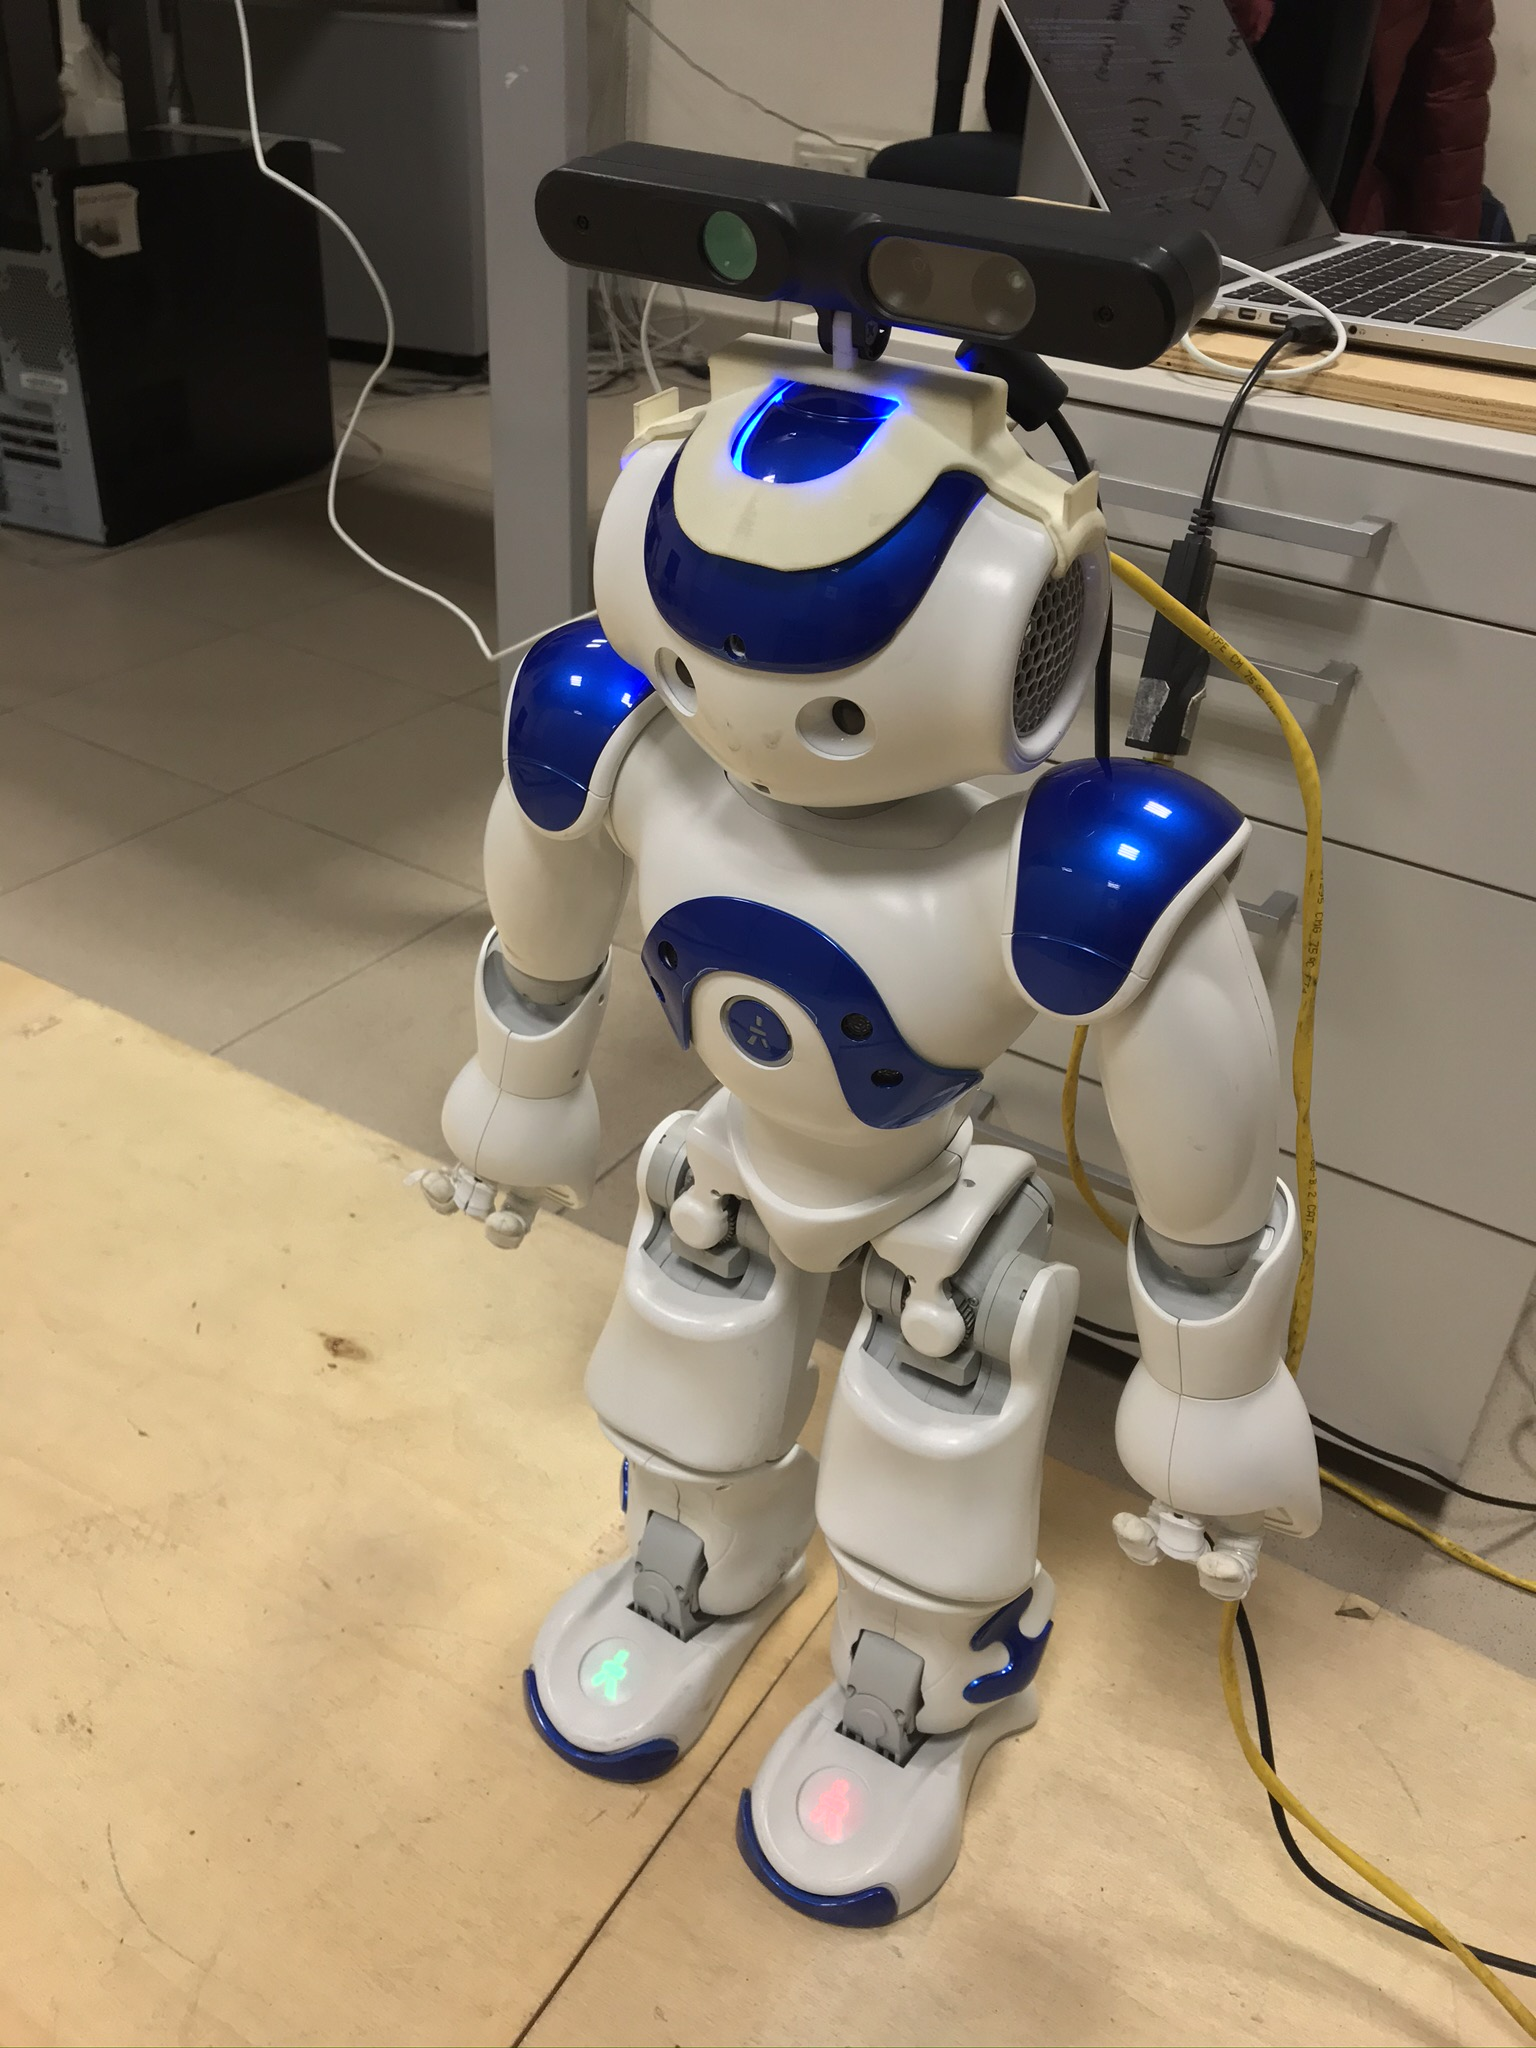
\includegraphics[width=0.5\textwidth]{figures/NAO-with-xtion-2.JPEG}
  \caption{The figure shows NAO v5 humanoid robot, the platform
      used for the experiments of this thesis, equipped with an ASUS Xtion
      Pro RGB-D camera. The camera is connected via USB to an external 
      computer which runs \texttt{elevation\_mapping} and the footstep 
      planner. The external computer communicates with NAO through an 
      ethernet cable using TCP.}
  \label{fig:nao-with-xtion-2}
\end{figure}

\section{Simple Staircase}
As mentioned before, the aim of the first experiment is to understand the kind 
of scenario that the robot can handle. In this first setting, only the robot 
with the Variable Height CoM IS-MPC is used. The planner and the mapper will 
be introduced later. The footsteps are, hence, assigned manually.

The first scenario, called ``Normal Staircase'' consists in placing the robot 
in front of a staircase of 2 cm in order to make the robot climb it.
To consider the experiment successful, NAO must climb the staircase 
putting the whole foot on the ground at each step. Increasing the length 
of the footstep increases the footprint area that is in contact with the ground 
at each step during climbing. However, while shorter footsteps are easier to 
perform, longer footsteps need to deal with the kinematic limitations of the 
robot. It is clear from the experiment (Fig.
\ref{fig:experiments:failing-normal-staircase:videoframes}) that the 
larger the footstep is, the harder it is for the robot to make a step. In 
particular, in Fig. \ref{fig:exp:fail:frame1} the robot performs a
footstep of size 16 cm; the foot is not placed entirely on the 
staircase (Fig. \ref{fig:exp:fail:frame2}), causing the robot to be unstable.
This causes the robot to slip (Fig. \ref{fig:exp:fail:frame3})
while attempting to do the second step. In the end, the robot
falls on the floor (Fig. \ref{fig:exp:fail:frame4}) failing the assigned task.
A longer footstep is, hence, needed in 
order to correctly perform the motion. However, due to the short legs of the 
robot, longer footsteps cause the robot to immediately fall. This suggests 
that NAO is not able to climb this kind of stairway due to its kinematics and 
that a special stairway needs to be built in order to test the behaviour of 
the Variable Height CoM IS-MPC.
\begin{figure}
  \begin{subfigure}{0.48\textwidth}
    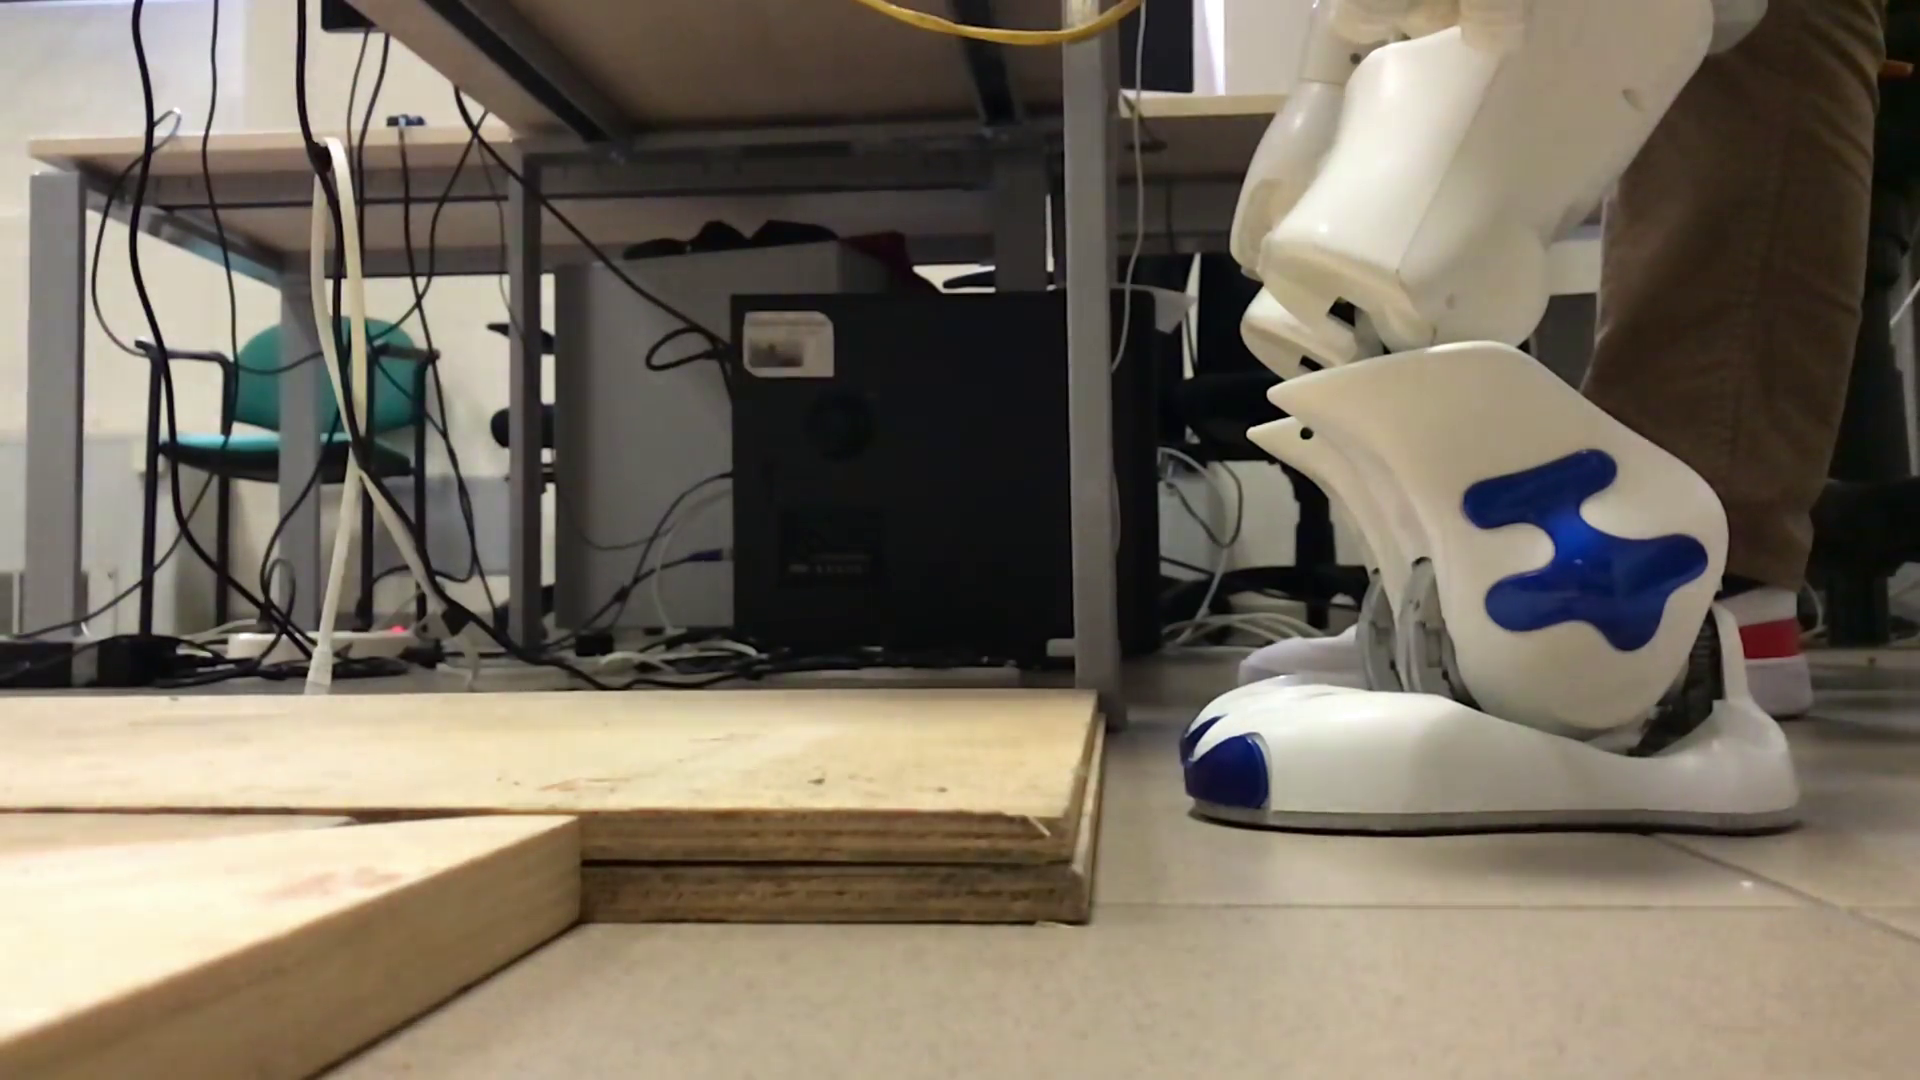
\includegraphics[width=\linewidth]
      {figures/experiments/failing-normal-staircase/video/01.png}
    \caption{Starting position}
    \label{fig:exp:fail:frame1}
  \end{subfigure}\hspace*{\fill}
  \begin{subfigure}{0.48\textwidth}
    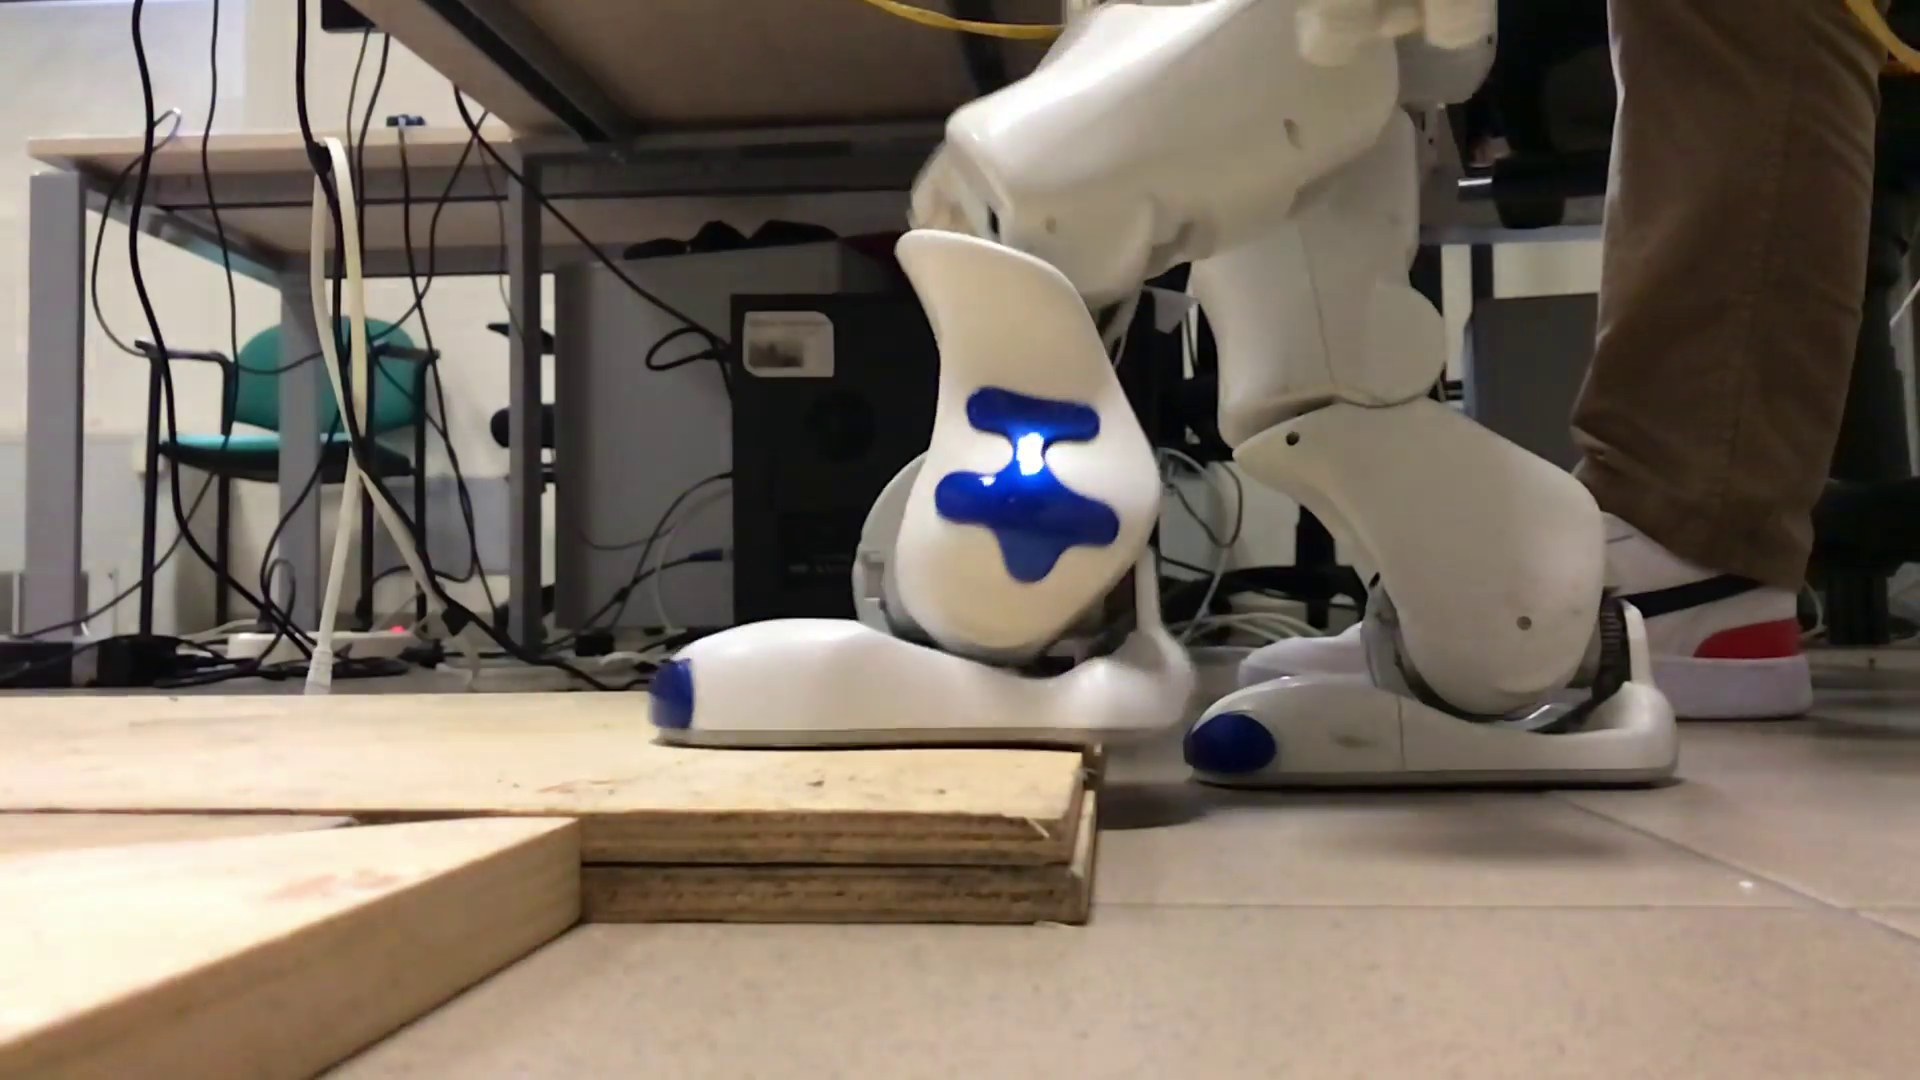
\includegraphics[width=\linewidth]
      {figures/experiments/failing-normal-staircase/video/02.png}
    \caption{First step}
    \label{fig:exp:fail:frame2}
  \end{subfigure}
  \begin{subfigure}{0.48\textwidth}
    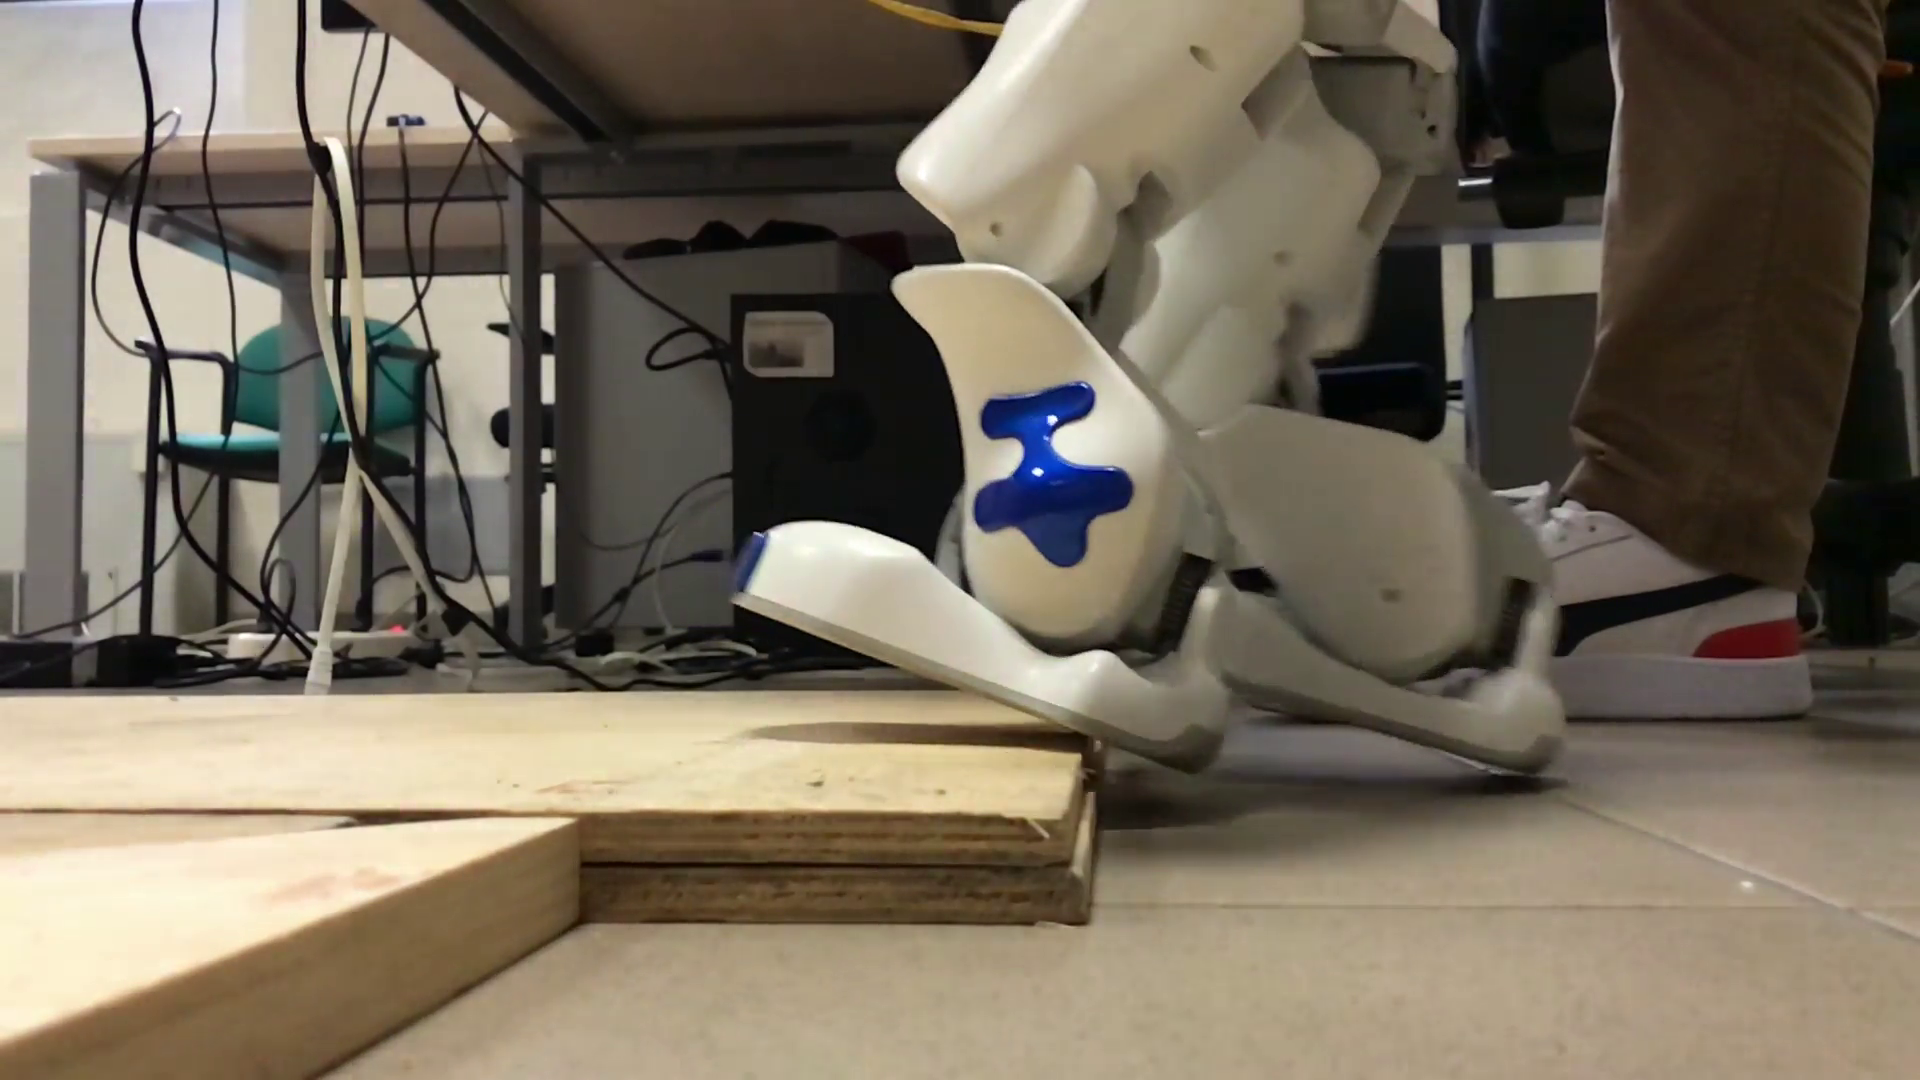
\includegraphics[width=\linewidth]
      {figures/experiments/failing-normal-staircase/video/03.png}
    \caption{Second step}
    \label{fig:exp:fail:frame3}
  \end{subfigure}\hspace*{\fill}
  \begin{subfigure}{0.48\textwidth}
    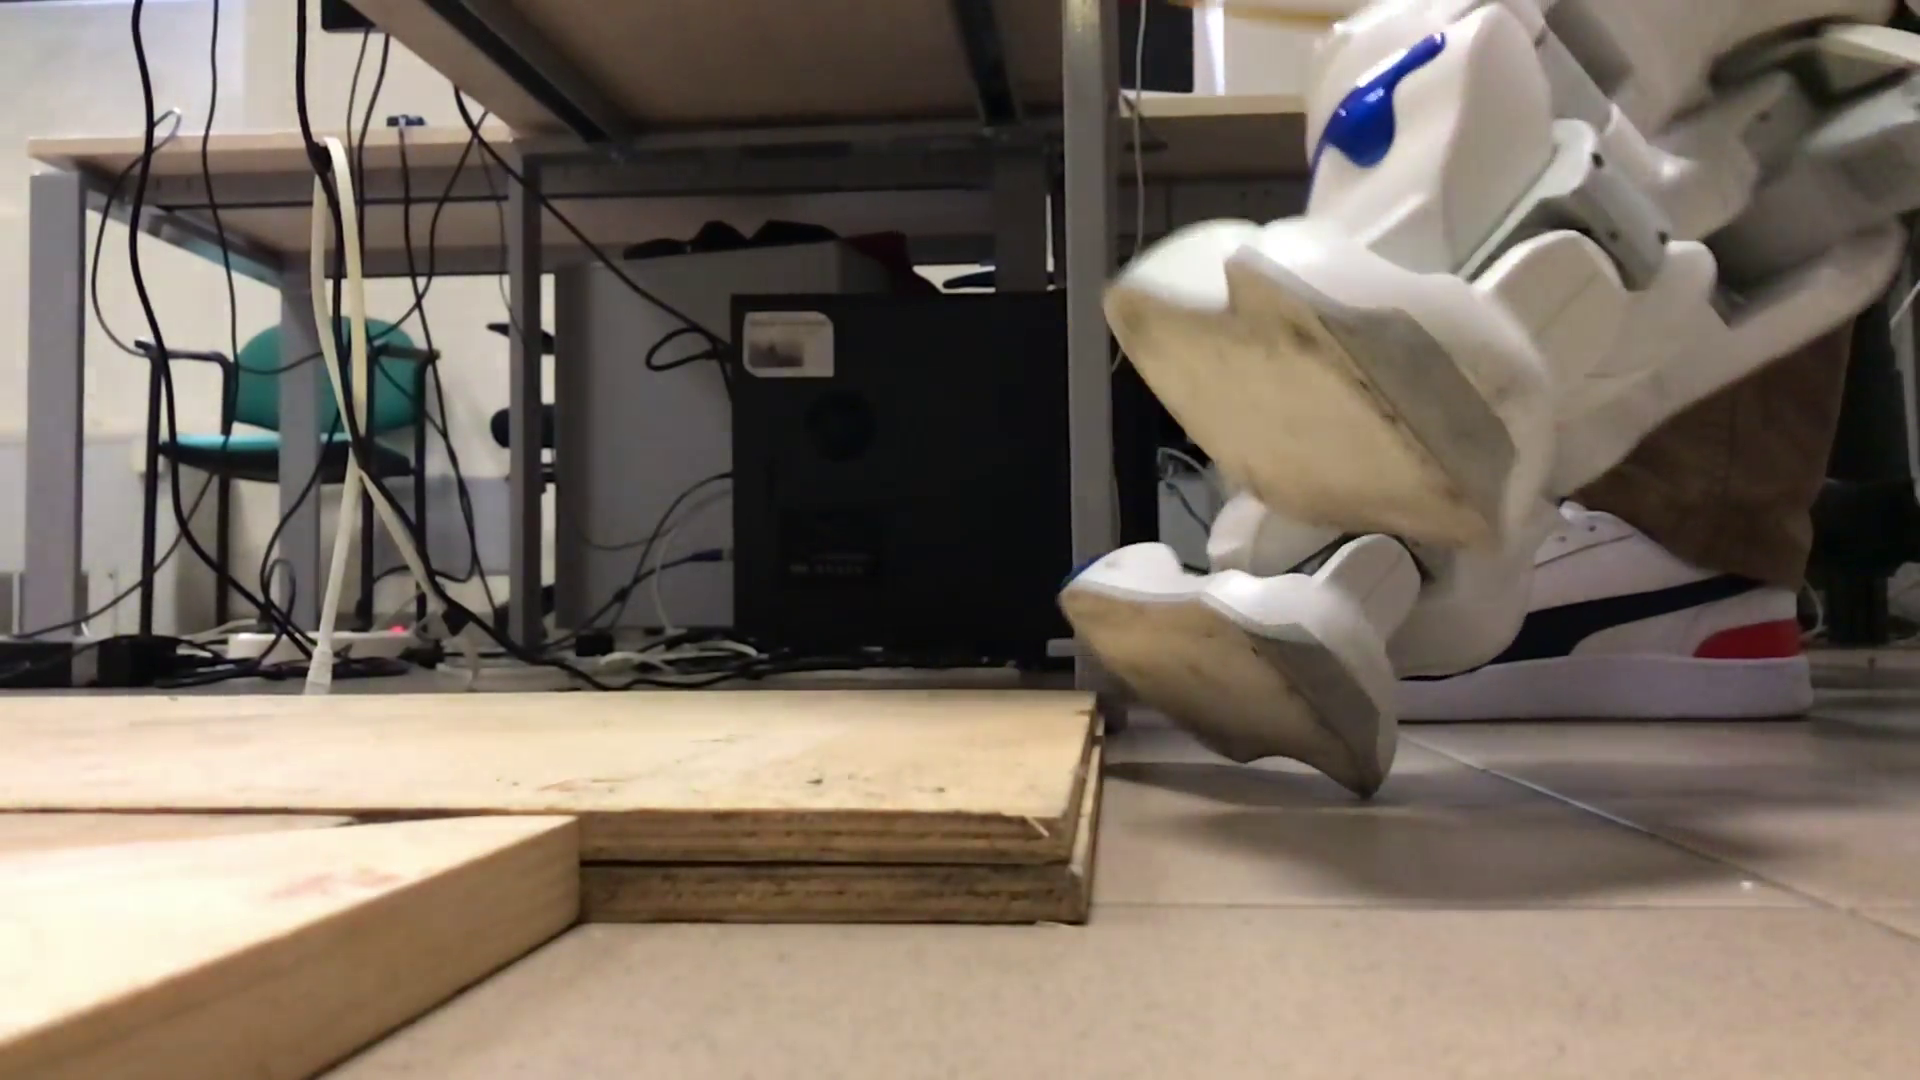
\includegraphics[width=\linewidth]
      {figures/experiments/failing-normal-staircase/video/04.png}
    \caption{Robot falling}
    \label{fig:exp:fail:frame4}
  \end{subfigure}
  \caption{The figures show the motion of the robot for the scenario ``Normal 
      Staircase''. The robot starts just in front of the stairs (Fig.
      \ref{fig:exp:fail:frame1}). The motion starts by placeing the first
      footstep on the staircase (Fig. \ref{fig:exp:fail:frame2}).
      Here, it is already clear that the motion could be unsuccessful. The foot 
      is, in fact, not entirely in contact with the staircase. Longer footsteps 
      make the robot immediately fall. Shorter footsteps are safer but fail to 
      correctly place the foot. In Fig. \ref{fig:exp:fail:frame3} the robot 
      attempts to place the other foot on the platform but it falls 
      (Fig. \ref{fig:exp:fail:frame4}), making the robot fail its task.
      Each staircase has a height of 2 cm.}
  \label{fig:experiments:failing-normal-staircase:videoframes}
\end{figure}

The scenario ``Simple Staircase'' is similar to the previous one. The only 
exception is the structure of the stairs, which has been put as in Fig.
\ref{fig:experiments:simple-staircase:videoframes} in order to give NAO 
some space to place the foot before climbing the staircase. Placing the 
staircases in this way allows the robot to perform climbing with shorter 
footsteps, avoiding kinematic limitations and correctly making it complete 
the assigned task. With these settings, NAO is able to climb staircases
up to 4 cm.
Fig. \ref{fig:experiments:simple-staircase:videoframes} shows NAO climbing 
a staircase of 3 cm. Fig. \ref{fig:experiments:simple-staircase:comzmp} shows 
how the CoM and the ZMP varies through time with respect to the position of the 
support foot, when dealing with a staircase of 4 cm. It is important to notice 
that both the CoM and the ZMP change their height when the robot performs a
step. This 
is possible because of the the Variable Height CoM IS-MPC described in Chapter 
\ref{ch:vh-com-is-mpc}, which allows the two variables to move along the $z$ 
axis while keeping a linear motion model like the Linear Inverted Pendulum
\cite{DBLP:conf/humanoids/SciancaCSLO16}. This characteristic is important 
not just in terms of the analysis of the system, but also in terms of 
computational resources, which can be kept low as for the case of NAO.
\begin{figure}
  \begin{subfigure}{0.48\textwidth}
    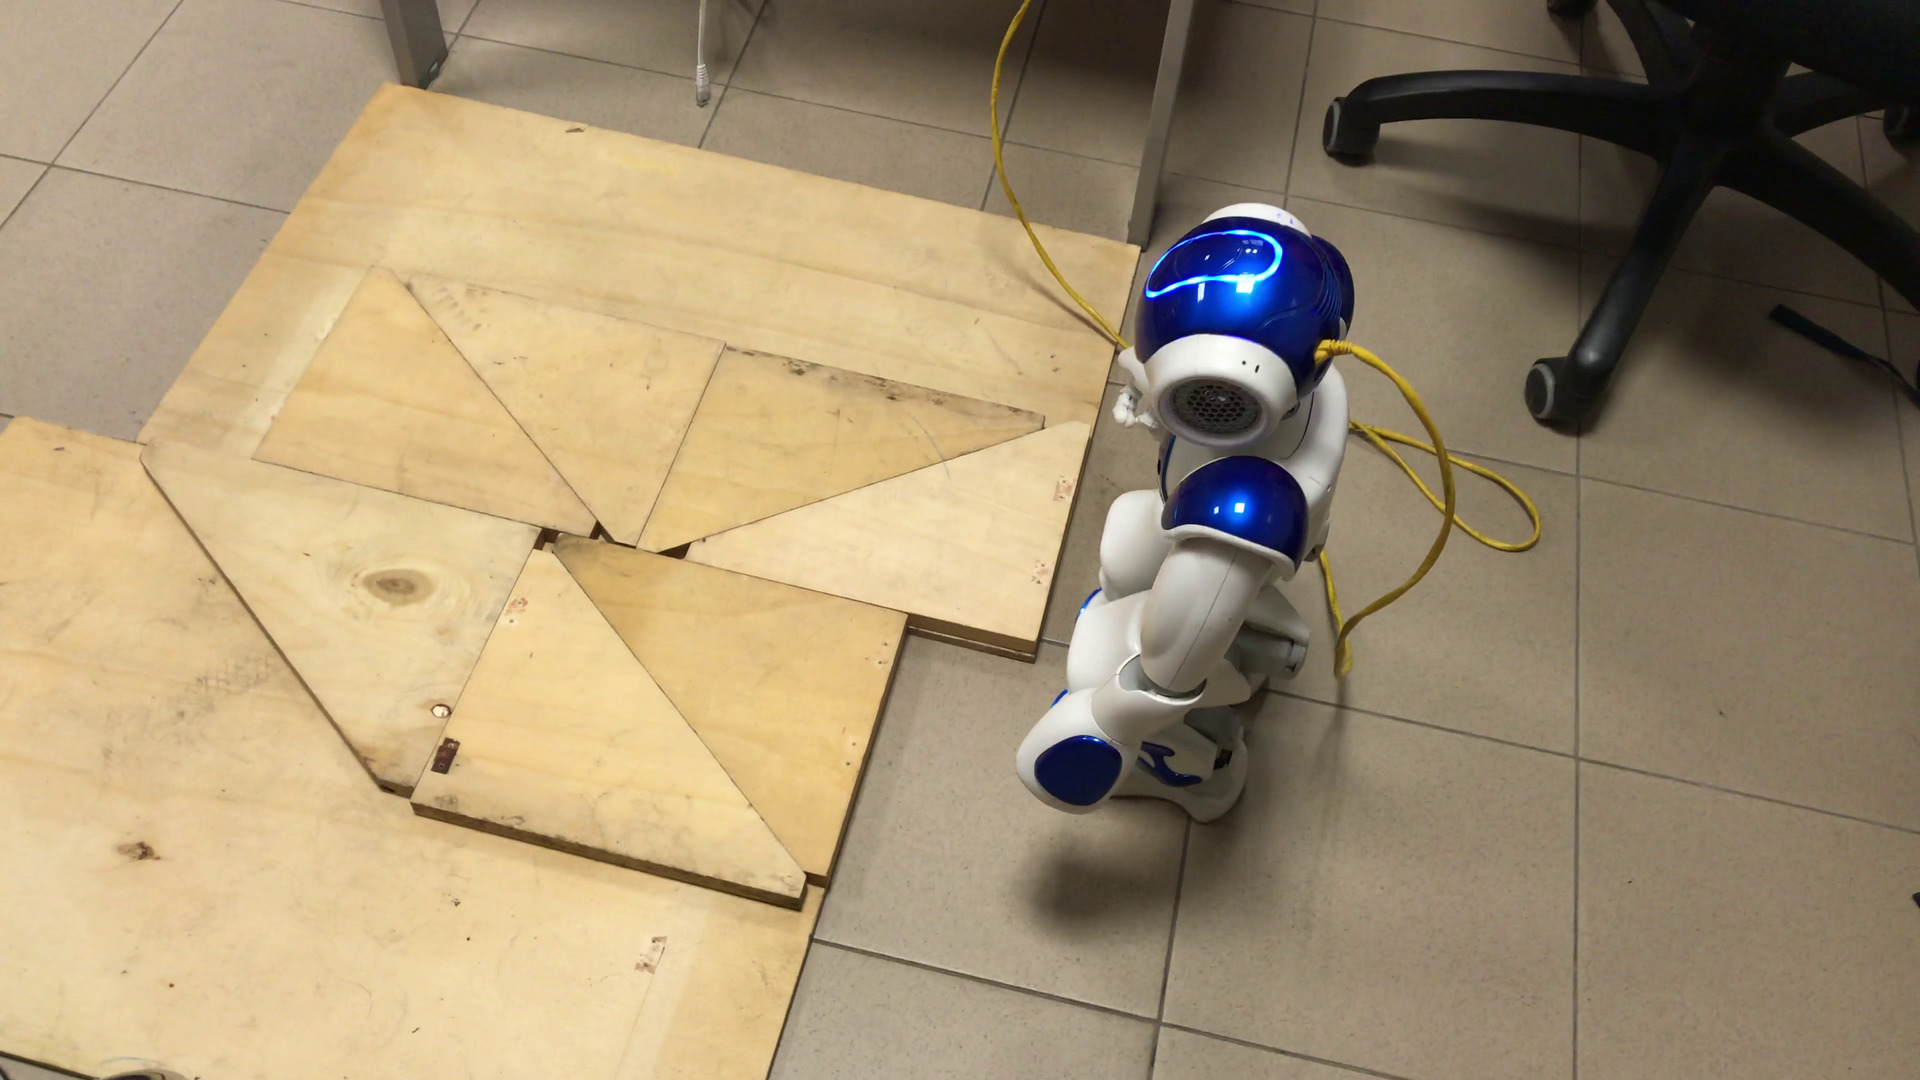
\includegraphics[width=\linewidth]
      {figures/experiments/simple-staircase/video/01.png}
    \caption{Starting position}
    \label{fig:exp:simple-staircase:frame1}
  \end{subfigure}\hspace*{\fill}
  \begin{subfigure}{0.48\textwidth}
    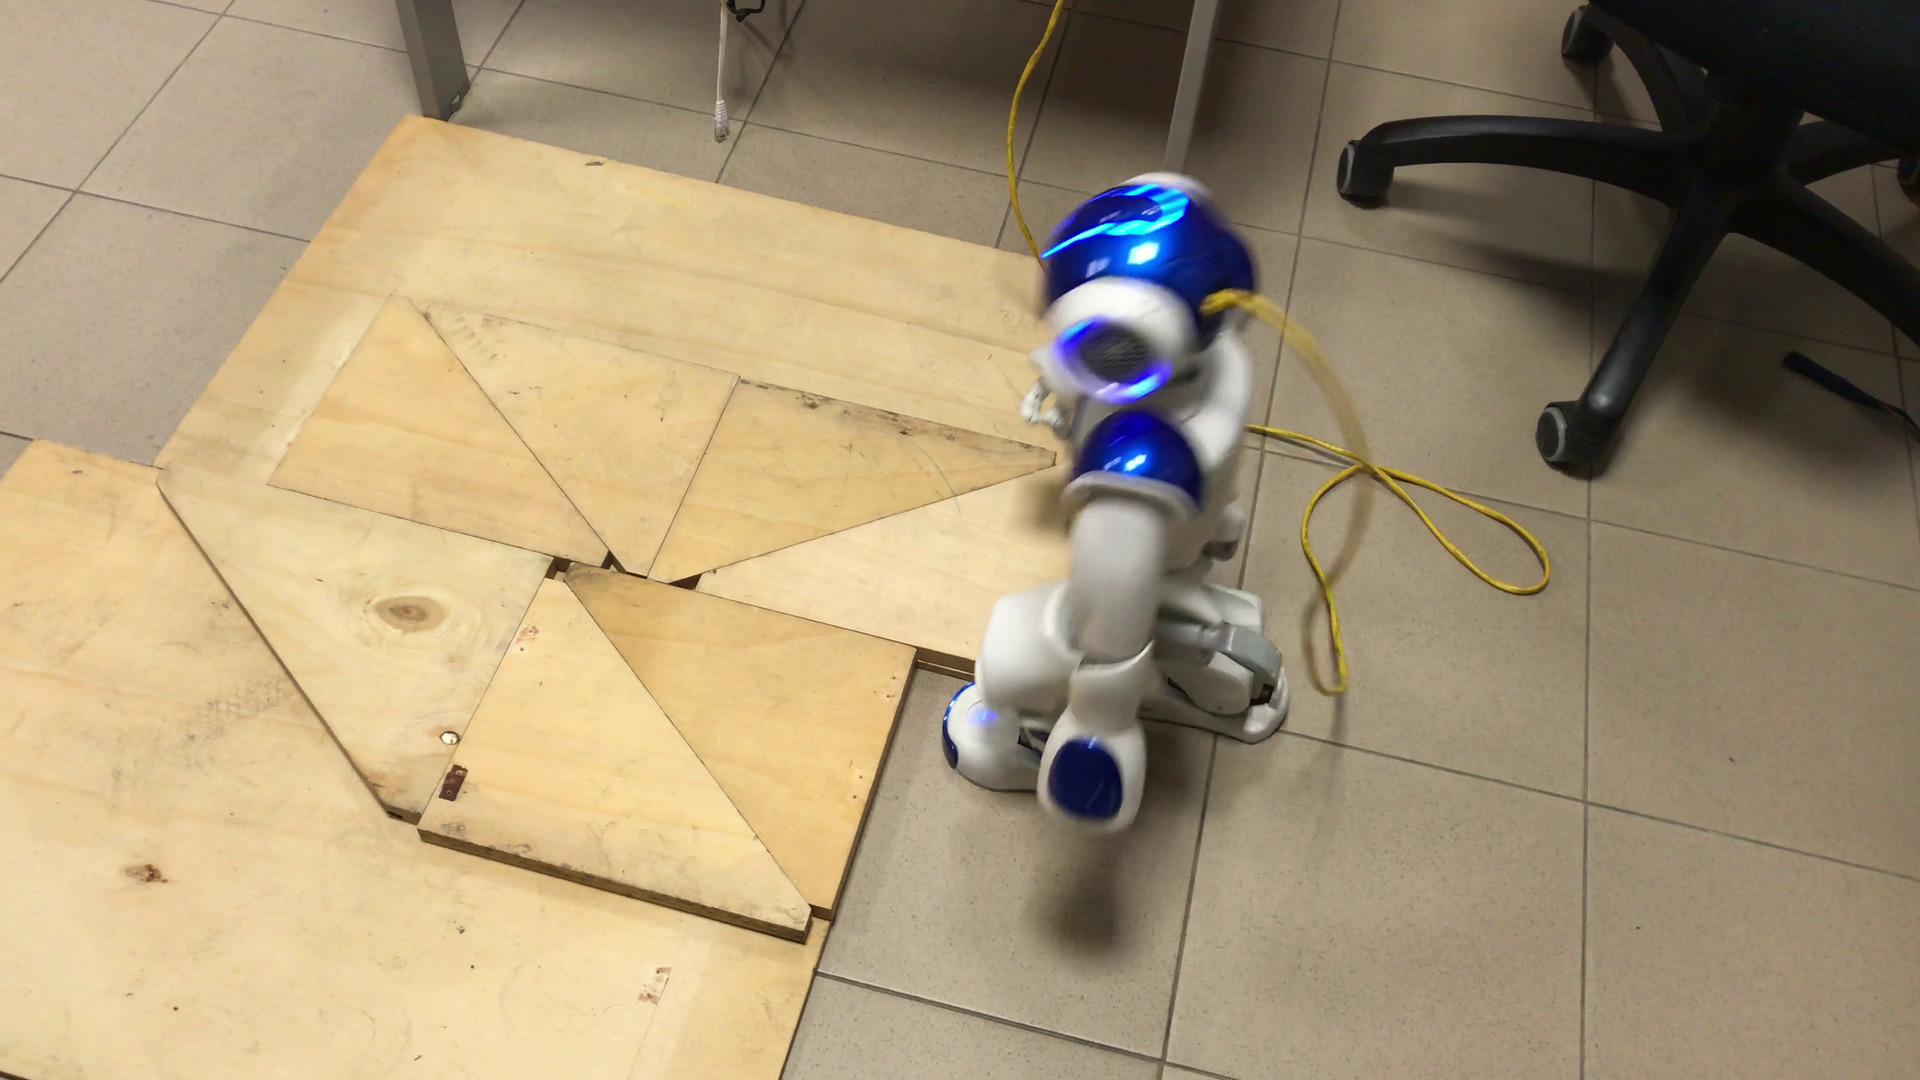
\includegraphics[width=\linewidth]
      {figures/experiments/simple-staircase/video/02.png}
    \caption{First step}
  \end{subfigure}
  \begin{subfigure}{0.48\textwidth}
    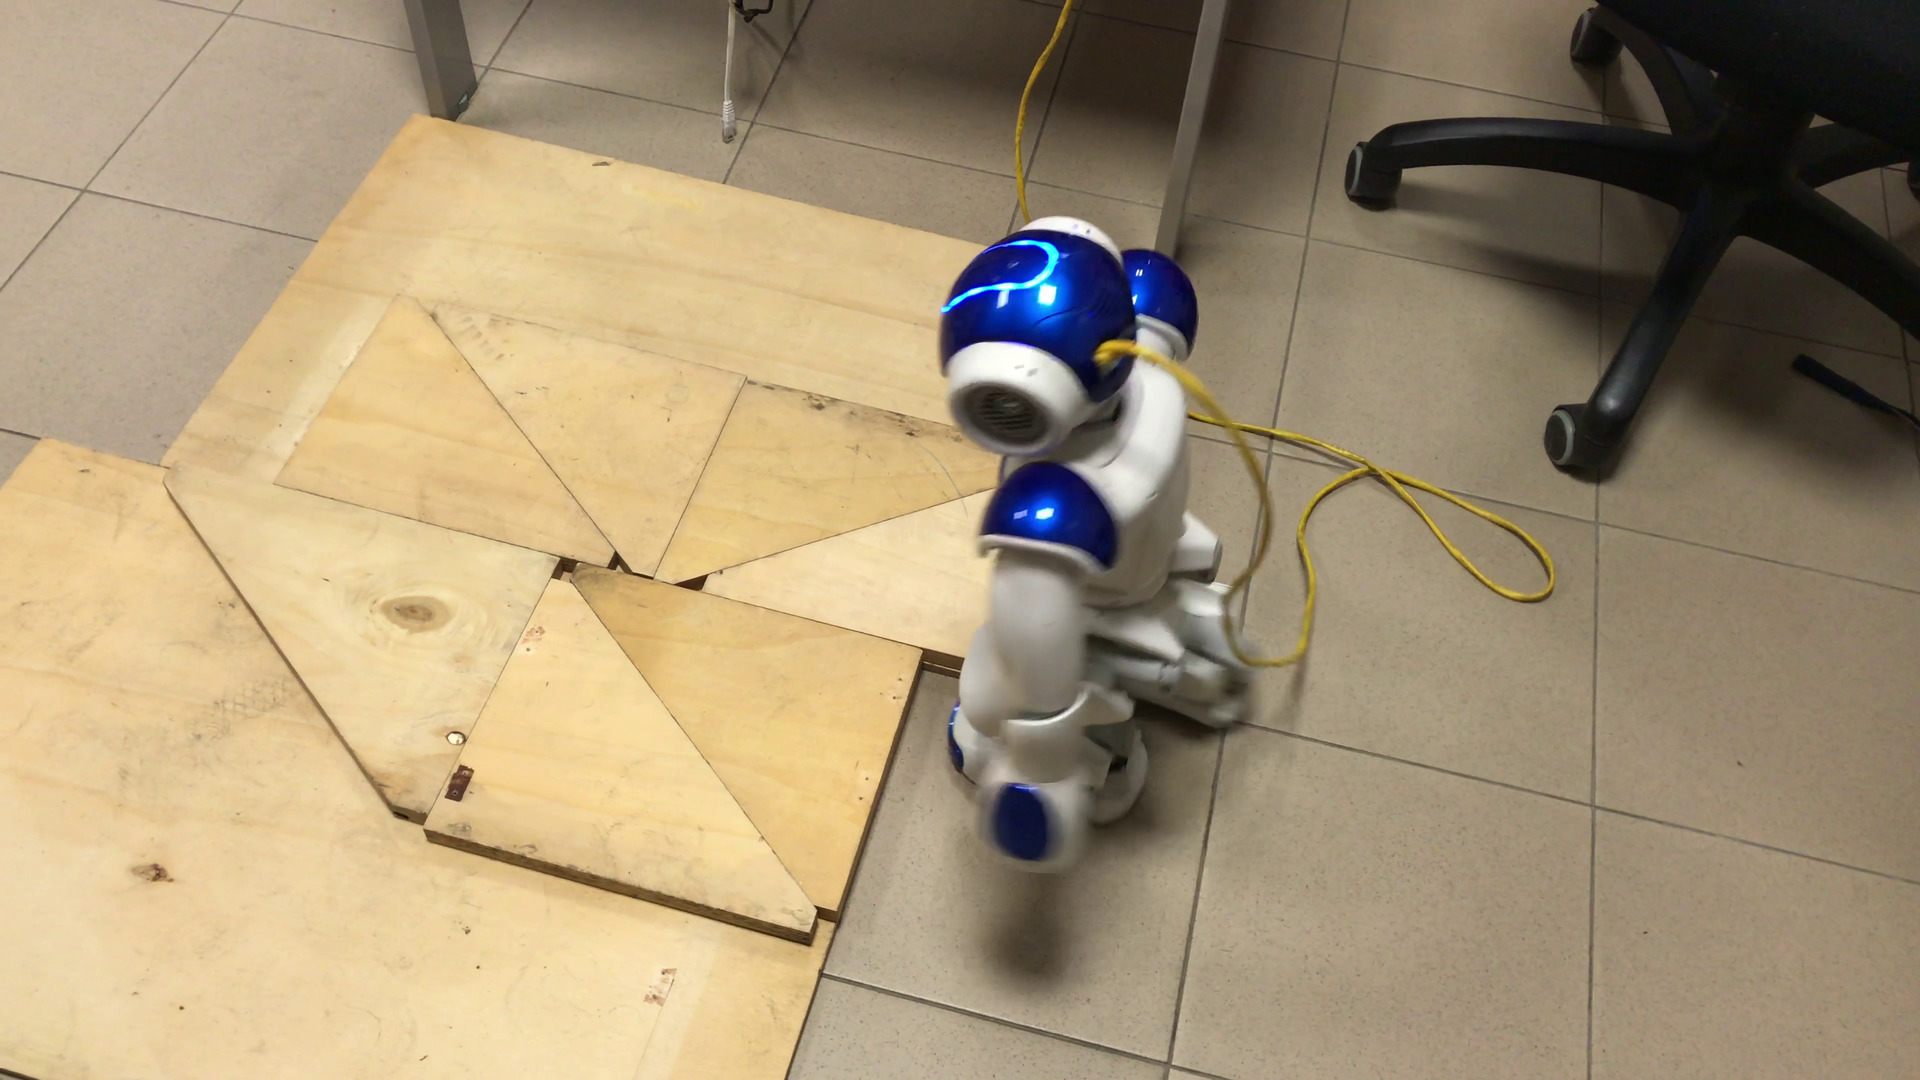
\includegraphics[width=\linewidth]
      {figures/experiments/simple-staircase/video/03.png}
    \caption{Second step}
  \end{subfigure}\hspace*{\fill}
  \begin{subfigure}{0.48\textwidth}
    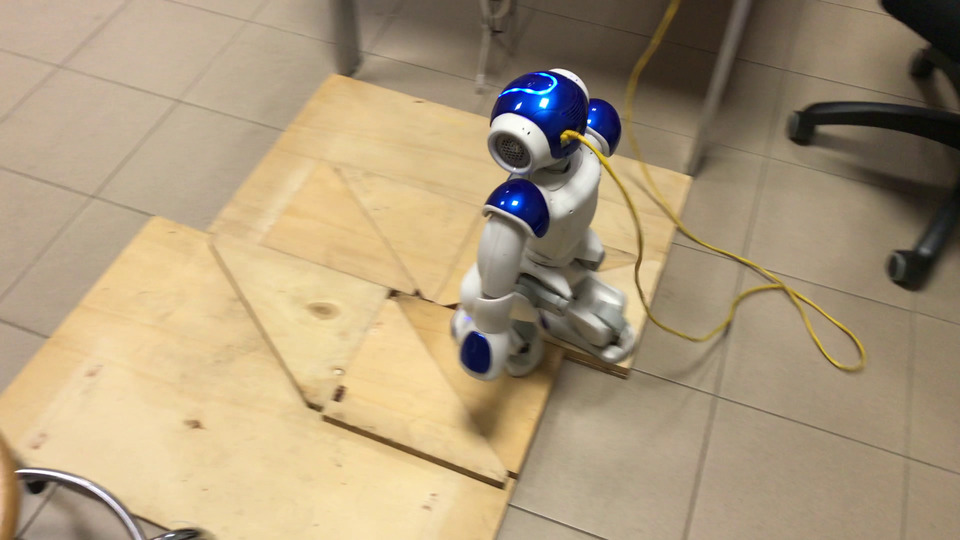
\includegraphics[width=\linewidth]
      {figures/experiments/simple-staircase/video/04.png}
    \caption{Third step}
  \end{subfigure}
  \begin{subfigure}{0.48\textwidth}
    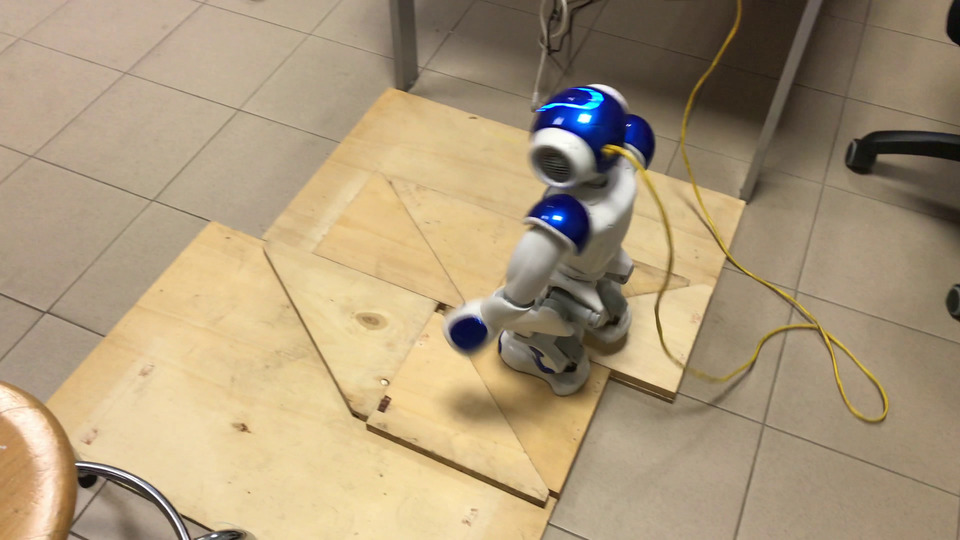
\includegraphics[width=\linewidth]
      {figures/experiments/simple-staircase/video/05.png}
    \caption{Fourth step}
  \end{subfigure}\hspace*{\fill}
  \begin{subfigure}{0.48\textwidth}
    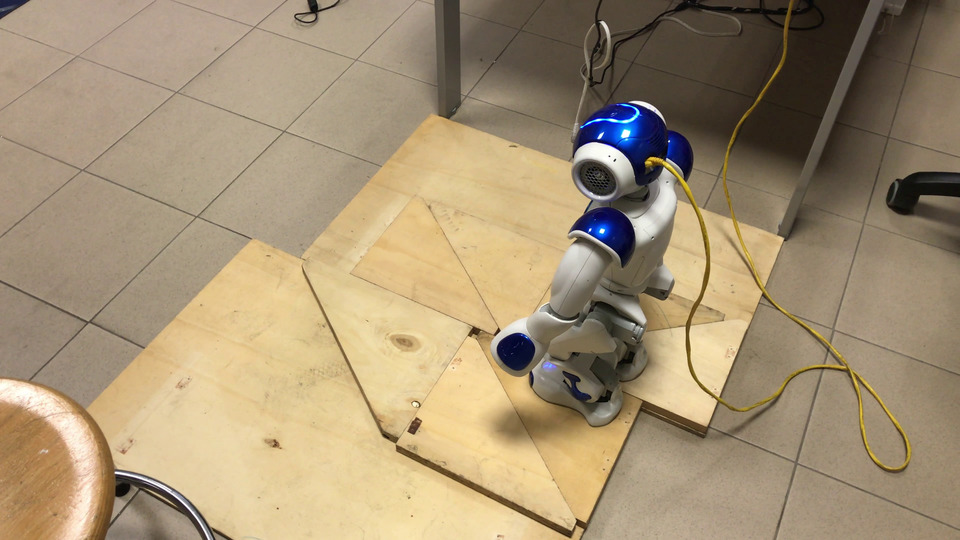
\includegraphics[width=\linewidth]
      {figures/experiments/simple-staircase/video/06.png}
    \caption{Final position}
  \end{subfigure} \caption{The figures show the motion of the robot for the 
      scenario ``Simple Staircase (3 cm)''. The robot start just in front of the 
      stairs (Fig. \ref{fig:exp:simple-staircase:frame1}), then it places 
      each step one in front of the other without colliding with the staircases,
      safely climbing the stairway. Each staircase has a height of 3 cm.}
  \label{fig:experiments:simple-staircase:videoframes}
\end{figure}
\begin{figure}
  \centering
  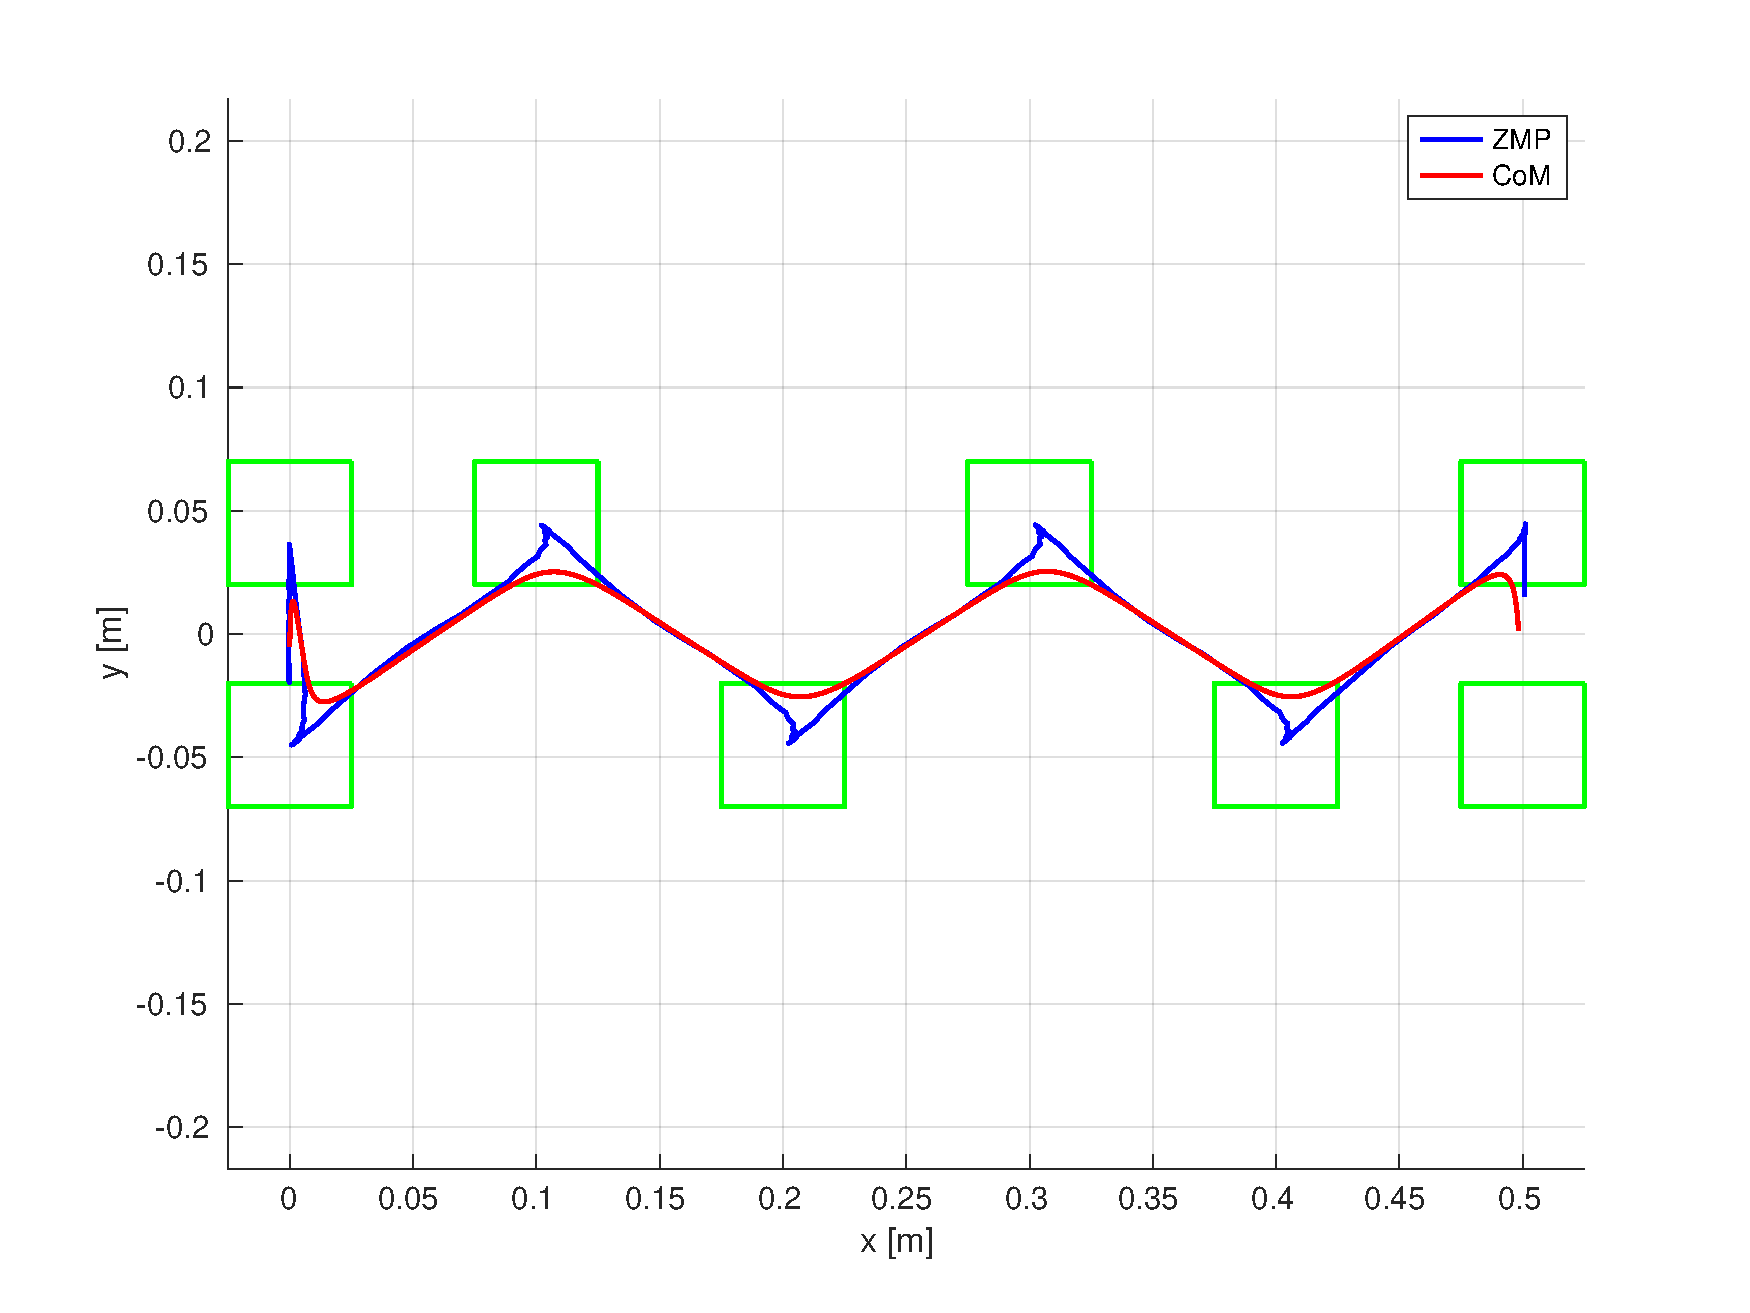
\includegraphics[width=\textwidth]
      {figures/experiments/simple-staircase/xy-plot-4cm.pdf}
  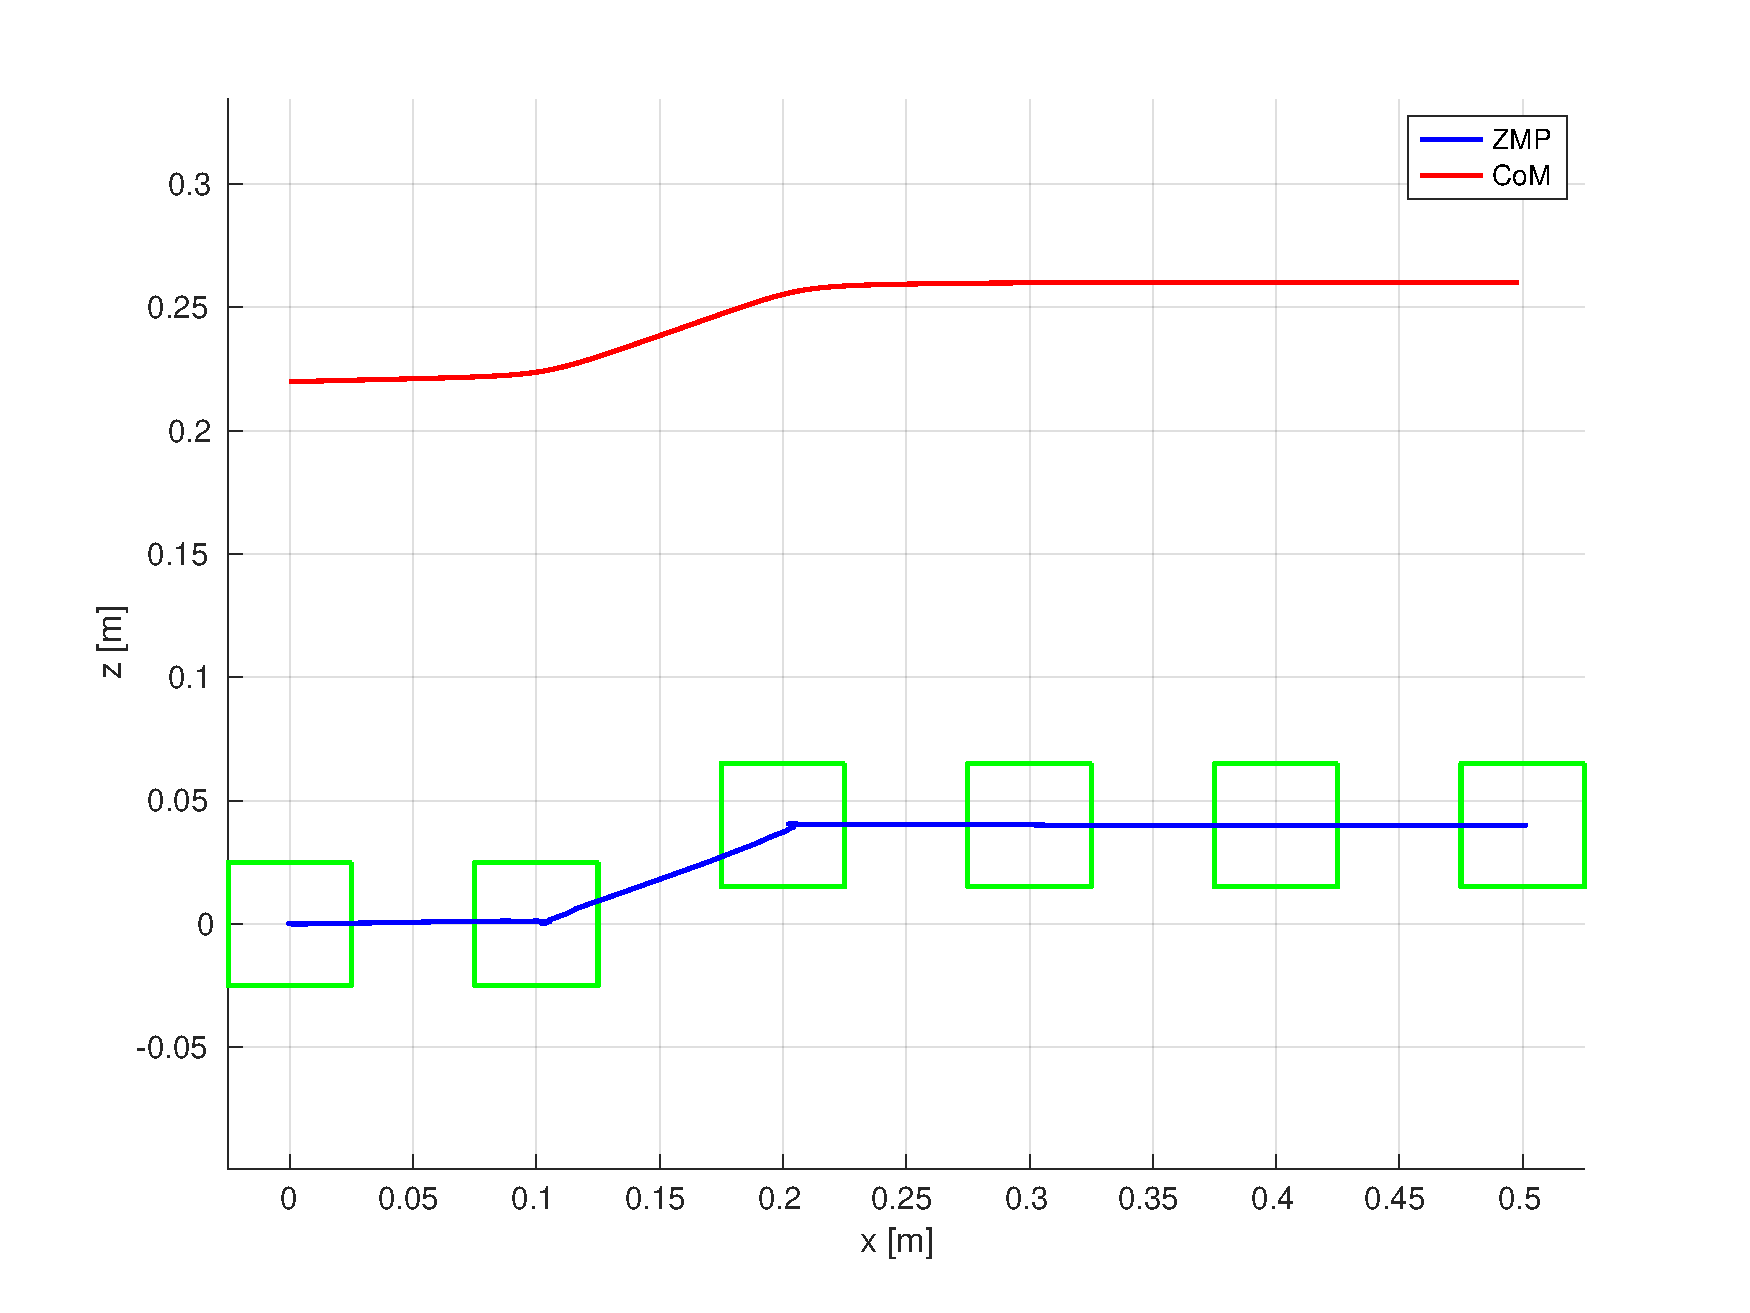
\includegraphics[width=\textwidth]
      {figures/experiments/simple-staircase/xz-plot-4cm.pdf}
  \caption{The plots show how the CoM and the ZMP vary with respect to the
		footsteps in the scenario ``Simple Staircase (4 cm)''.
    The green boxes represent the footsteps.}
  \label{fig:experiments:simple-staircase:comzmp}
\end{figure}

\section{Multiple Staircases}
This second experiment consists in making NAO climb a stairway composed of 
two staircases of 2 cm both upstairs and downstairs. The sequence of footsteps 
is manually assigned as in the previous experiment.

\subsection{Upstairs}
The following scenario is called ``Multiple Staircases (Upstairs)'' and it 
consists in making NAO climb a stairway composed of two consecutive staircases 
of 2 cm by moving upstairs. Fig.
\ref{fig:experiments:multiple-staircases:upstairs:videoframes} shows the 
behaviour of the robot for this setting. NAO correctly completes the assigned 
task reaching the top of the stairway. Fig. 
\ref{fig:experiments:multiple-staircases:upstairs:comzmp} show how the CoM and 
the ZMP changes through time during this experiment. Again, it is important to 
notice how both variables change in the $z$ axis, allowing the robot to 
safely climb the stairway.
\begin{figure}
  \begin{subfigure}{0.48\textwidth}
    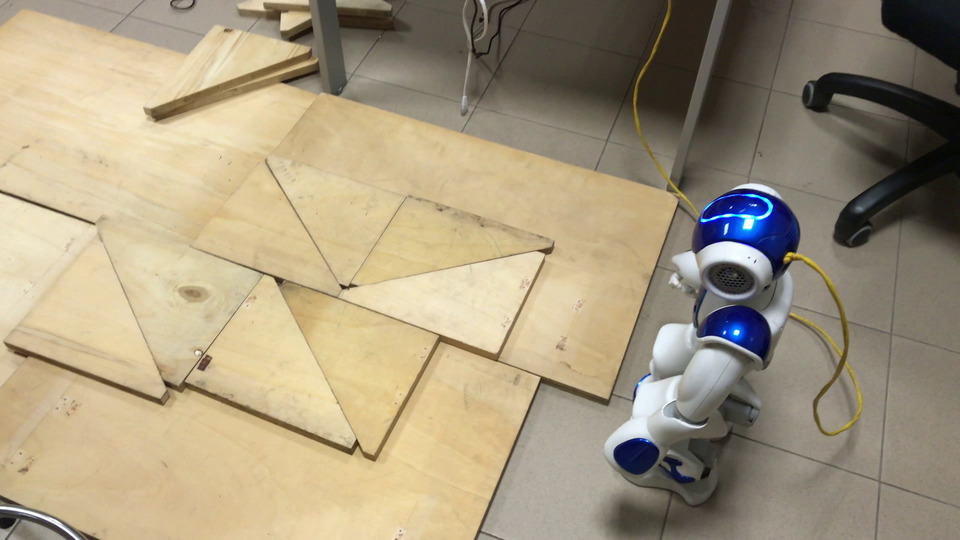
\includegraphics[width=\linewidth]
      {figures/experiments/multiple-staircases/upstairs/video/01.png}
    \caption{Starting position}
    \label{fig:exp:ms:up:frame1}
  \end{subfigure}\hspace*{\fill}
  \begin{subfigure}{0.48\textwidth}
    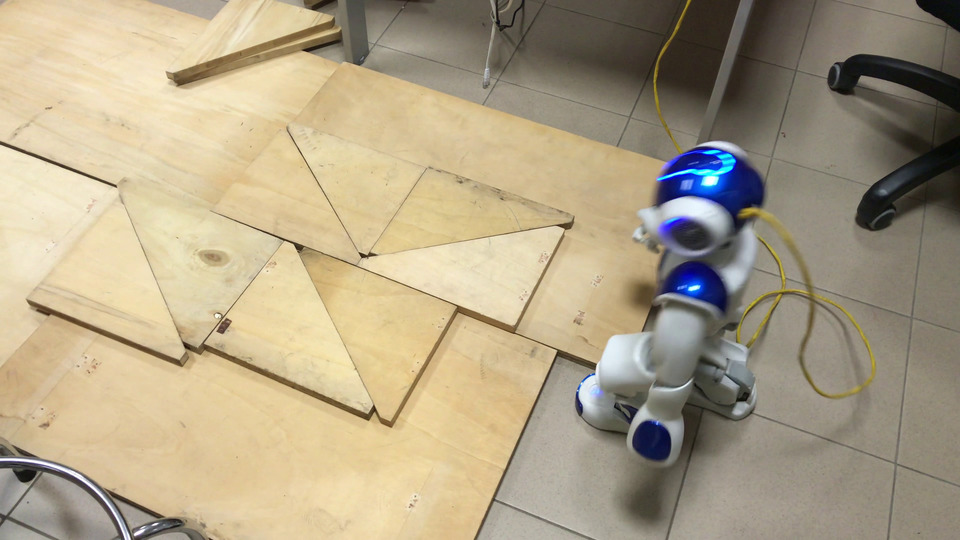
\includegraphics[width=\linewidth]
      {figures/experiments/multiple-staircases/upstairs/video/02.png}
    \caption{First step}
  \end{subfigure}
  \begin{subfigure}{0.48\textwidth}
    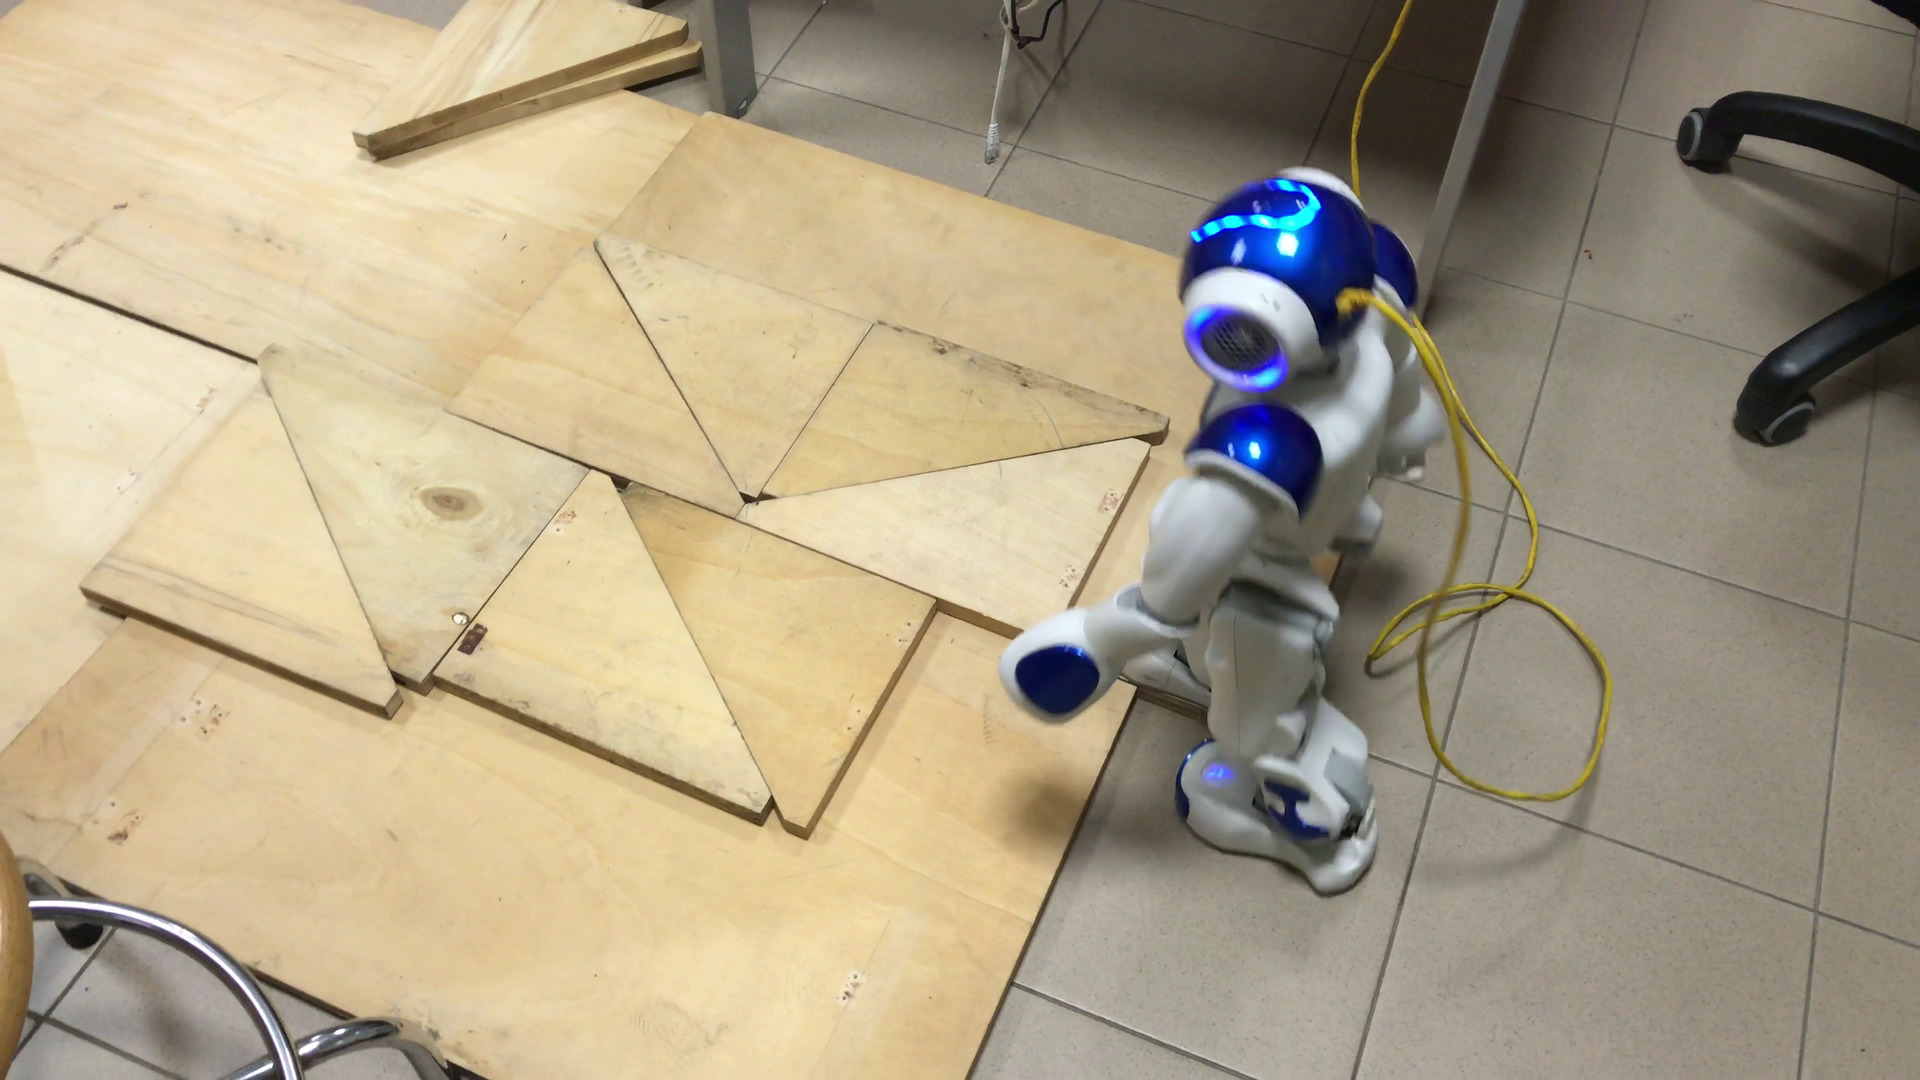
\includegraphics[width=\linewidth]
      {figures/experiments/multiple-staircases/upstairs/video/03.png}
    \caption{Second step}
  \end{subfigure}\hspace*{\fill}
  \begin{subfigure}{0.48\textwidth}
    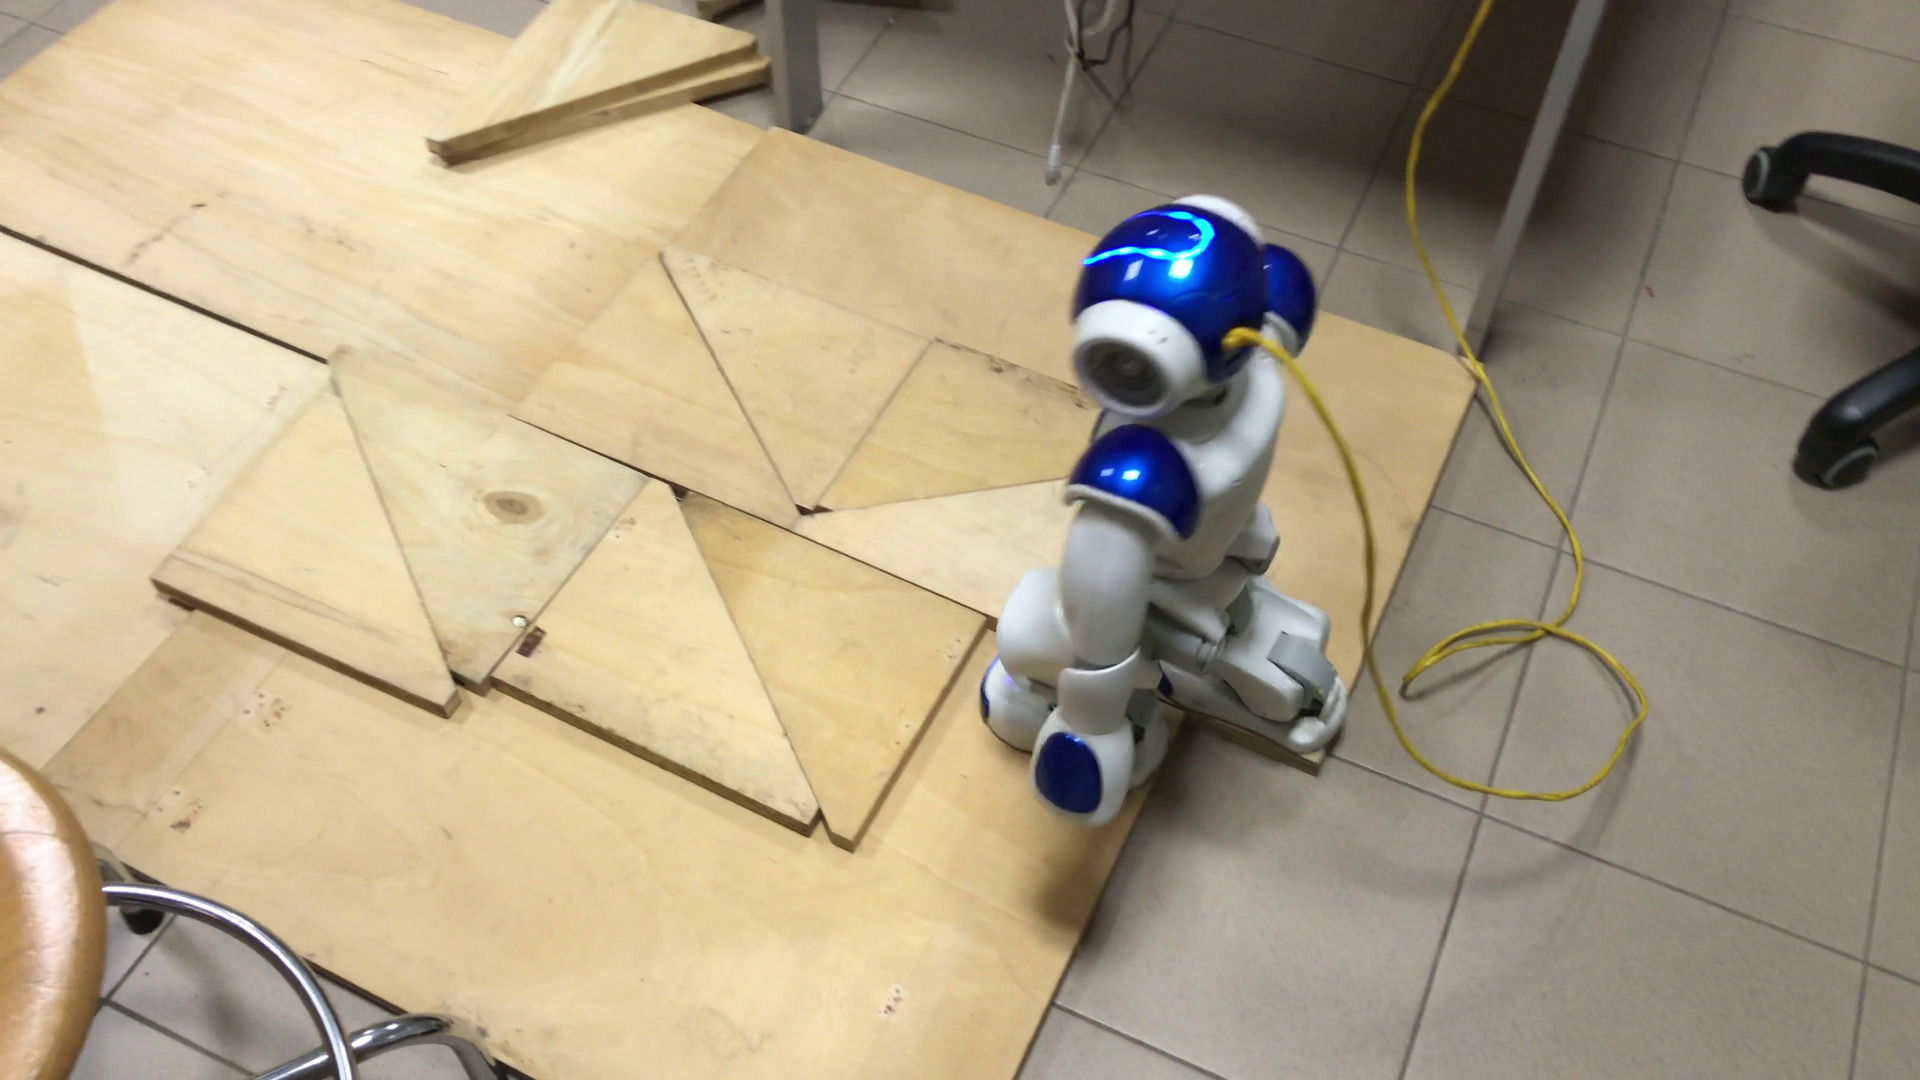
\includegraphics[width=\linewidth]
      {figures/experiments/multiple-staircases/upstairs/video/04.png}
    \caption{Third step}
  \end{subfigure}
  \begin{subfigure}{0.48\textwidth}
    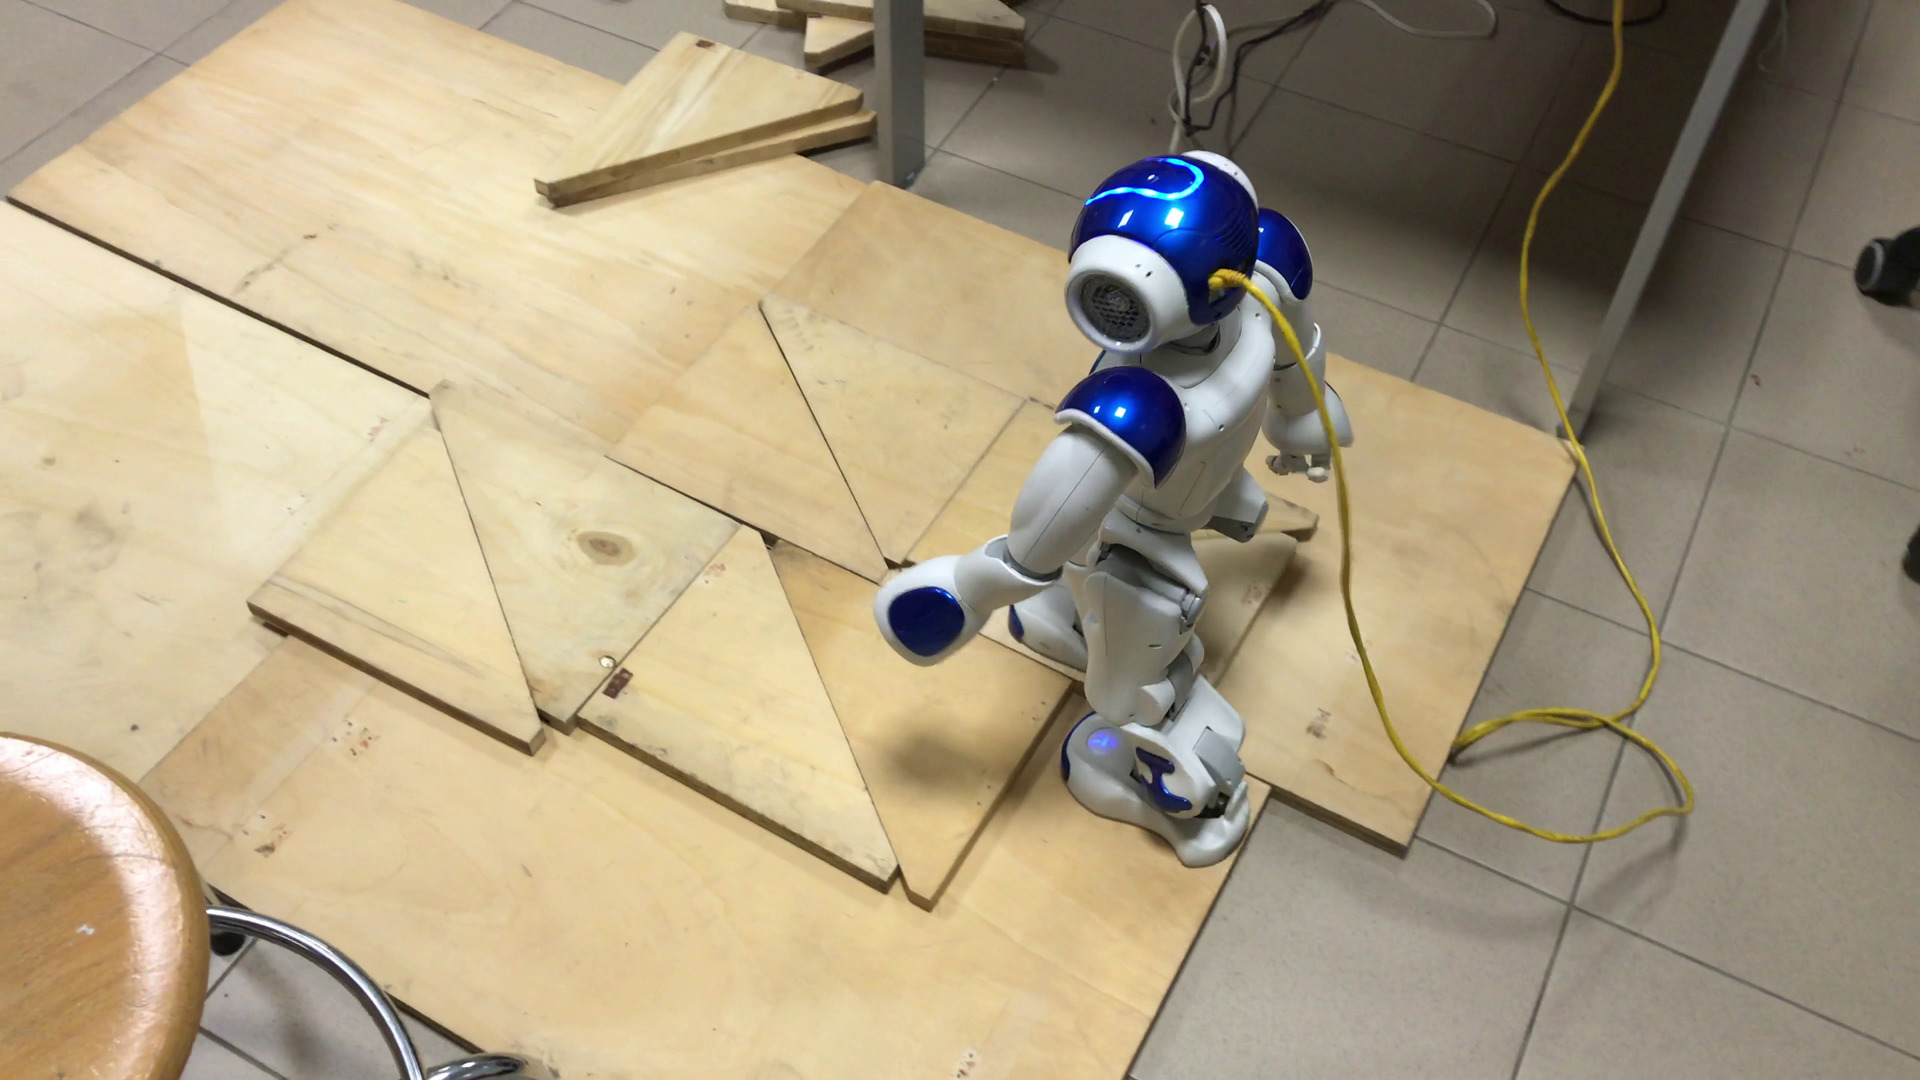
\includegraphics[width=\linewidth]
      {figures/experiments/multiple-staircases/upstairs/video/05.png}
    \caption{Fourth step}
  \end{subfigure}\hspace*{\fill}
  \begin{subfigure}{0.48\textwidth}
    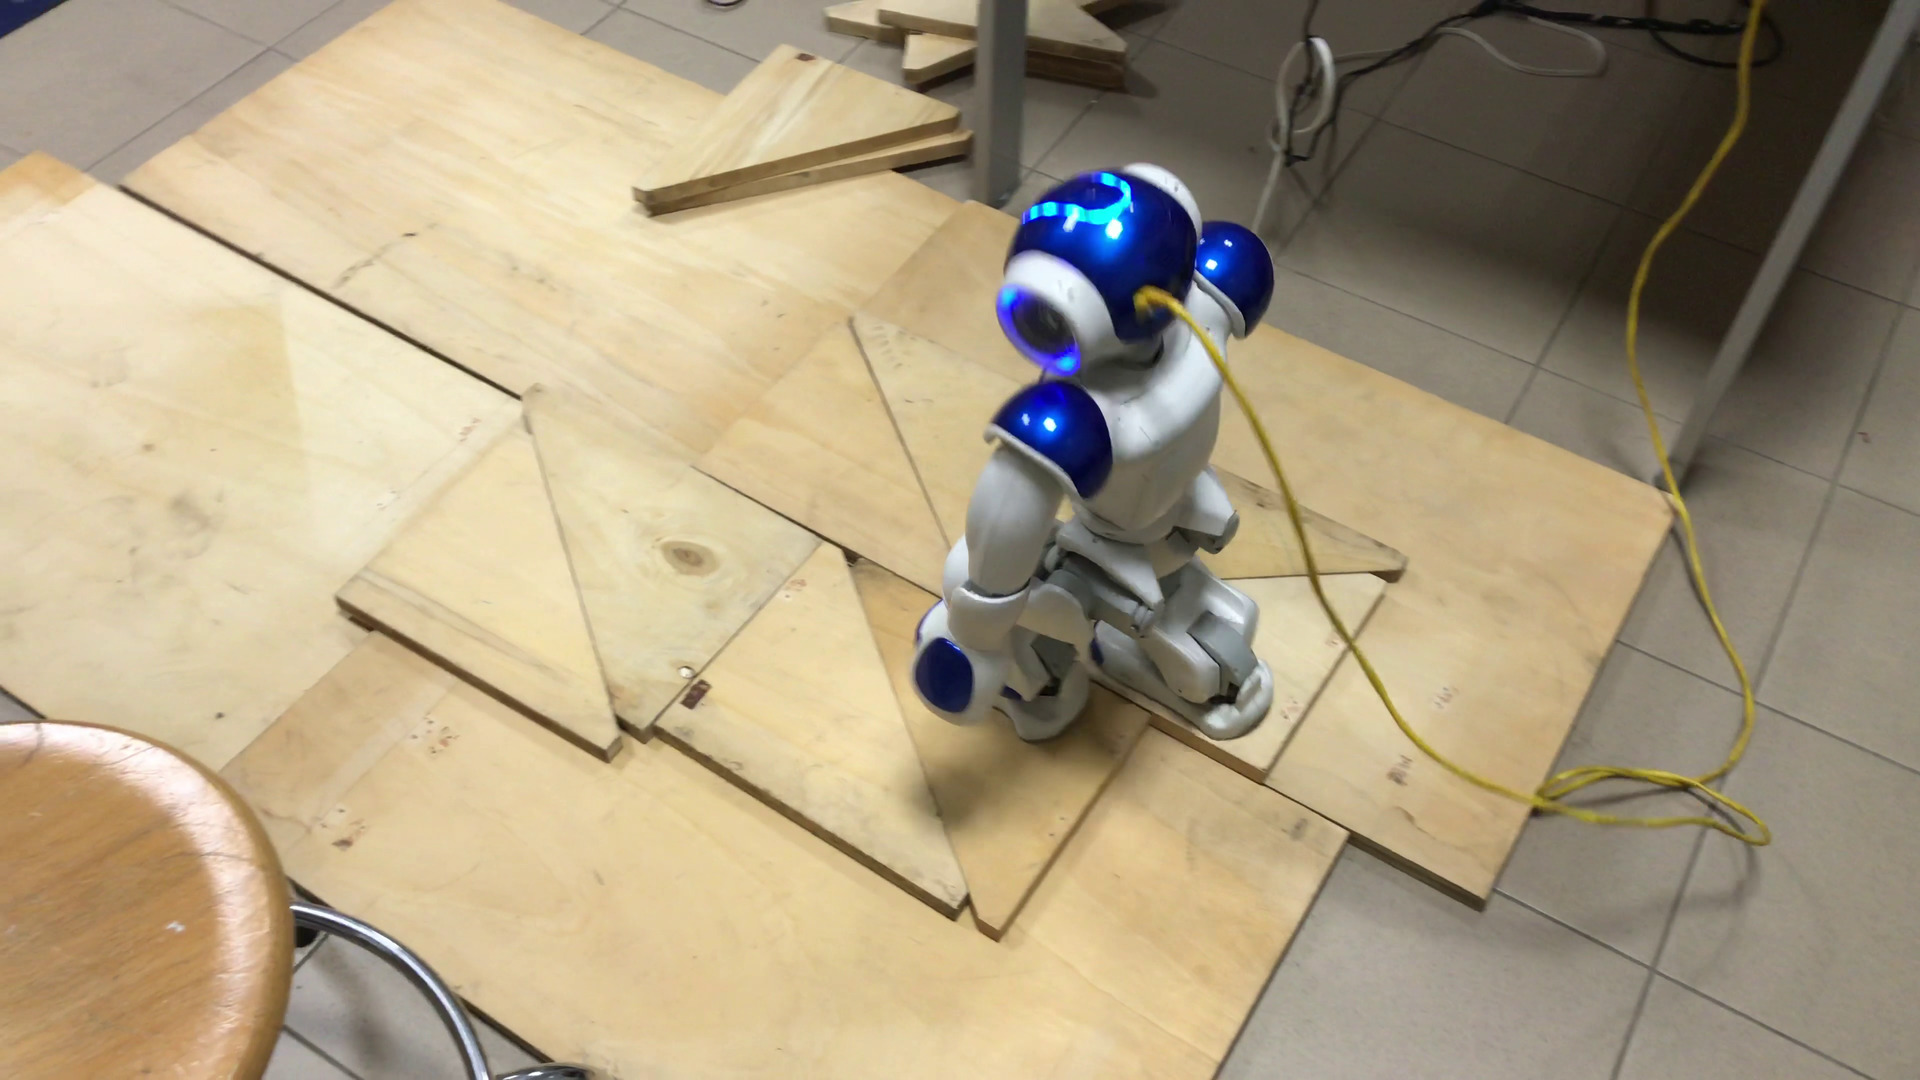
\includegraphics[width=\linewidth]
      {figures/experiments/multiple-staircases/upstairs/video/06.png}
    \caption{Fifth step}
  \end{subfigure}
  \caption{The figures show the motion of the robot for the scenario
      ``Multiple Staircases (Upstairs)''. The robot starts just in 
      front of the stairs (Fig. \ref{fig:exp:ms:up:frame1}), then it places 
      each step one in front of the other without colliding with the staircases,
      safely climbing the stairway. Each staircase has a height of 2 cm.}
  \label{fig:experiments:multiple-staircases:upstairs:videoframes}
\end{figure}

\begin{figure}
  \centering
  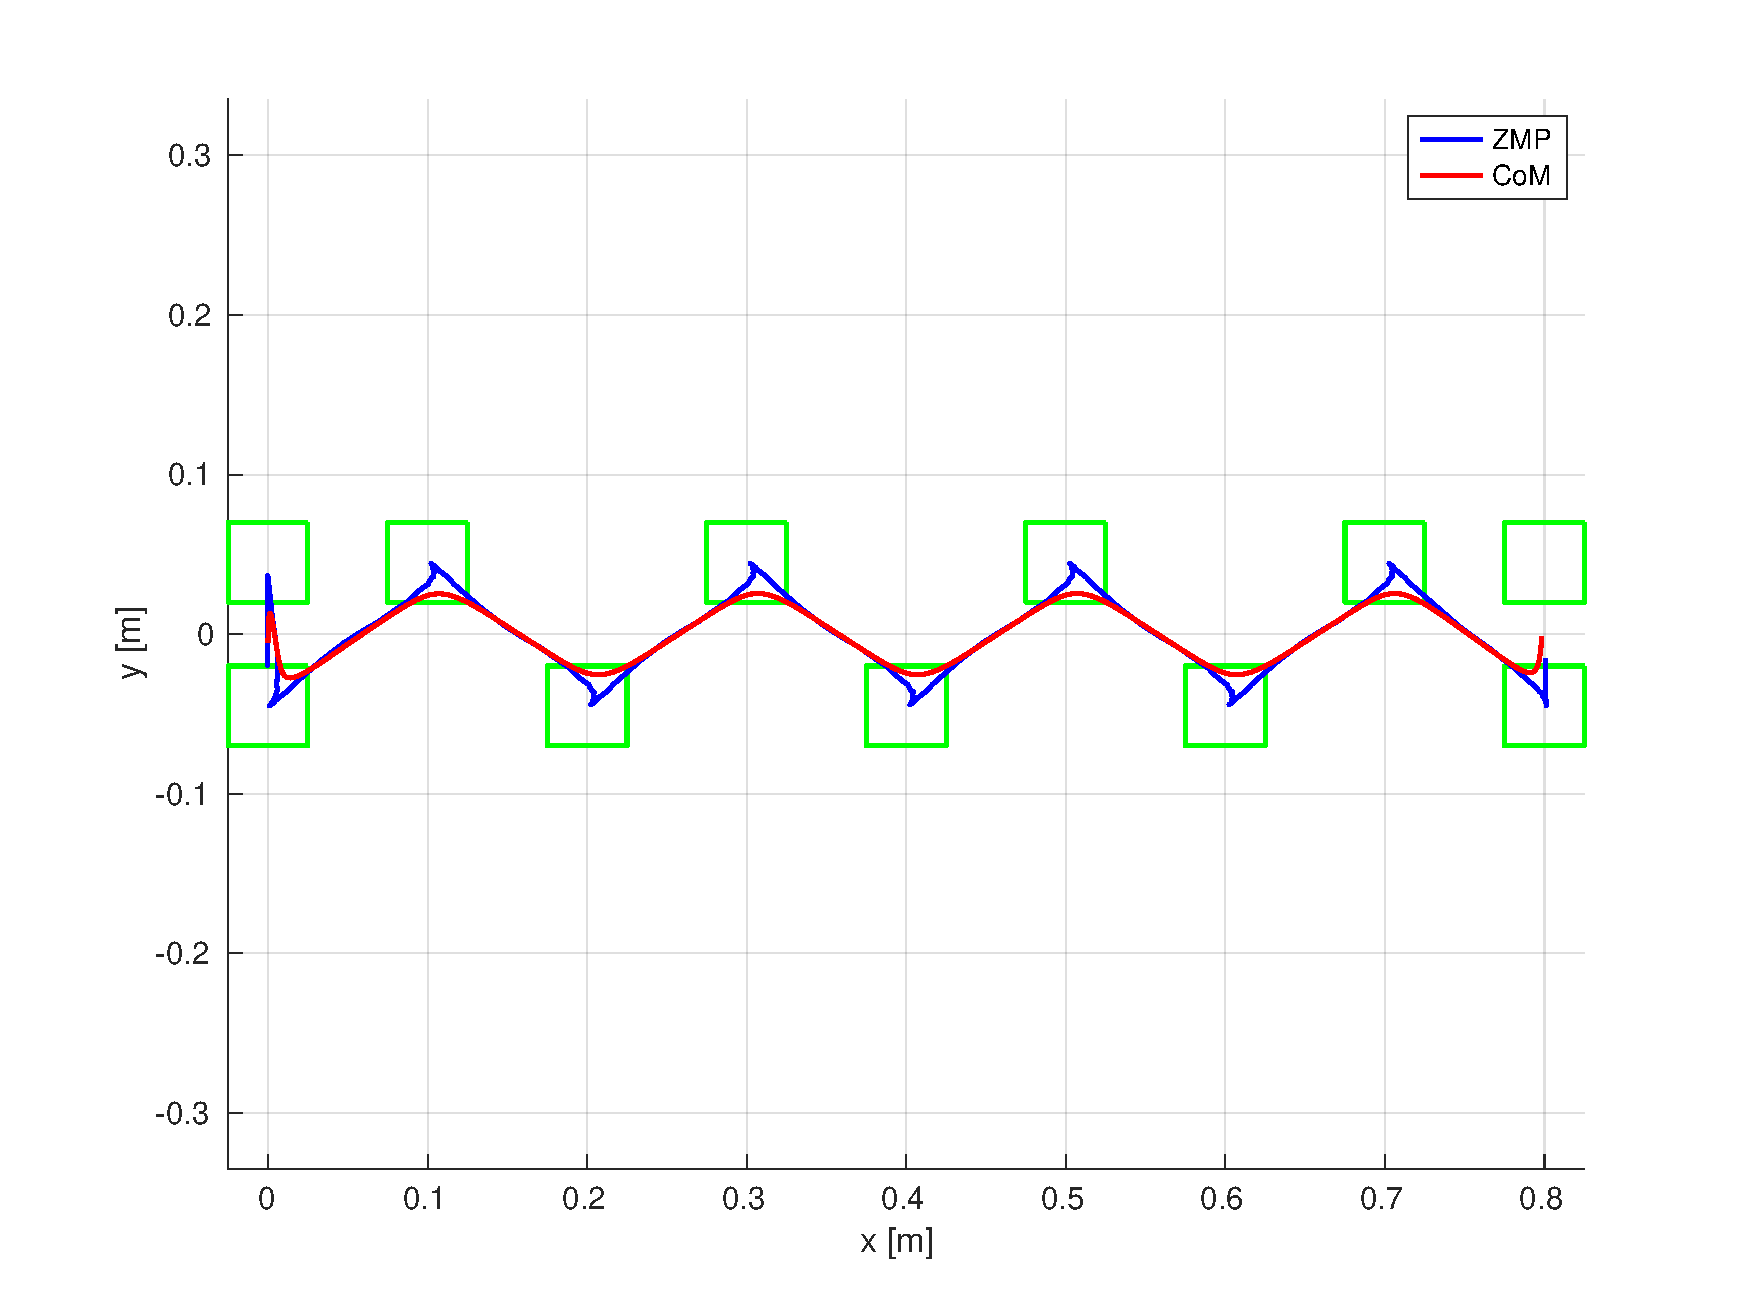
\includegraphics[width=\textwidth]
      {figures/experiments/multiple-staircases/upstairs/xy-plot-2cm.pdf}
  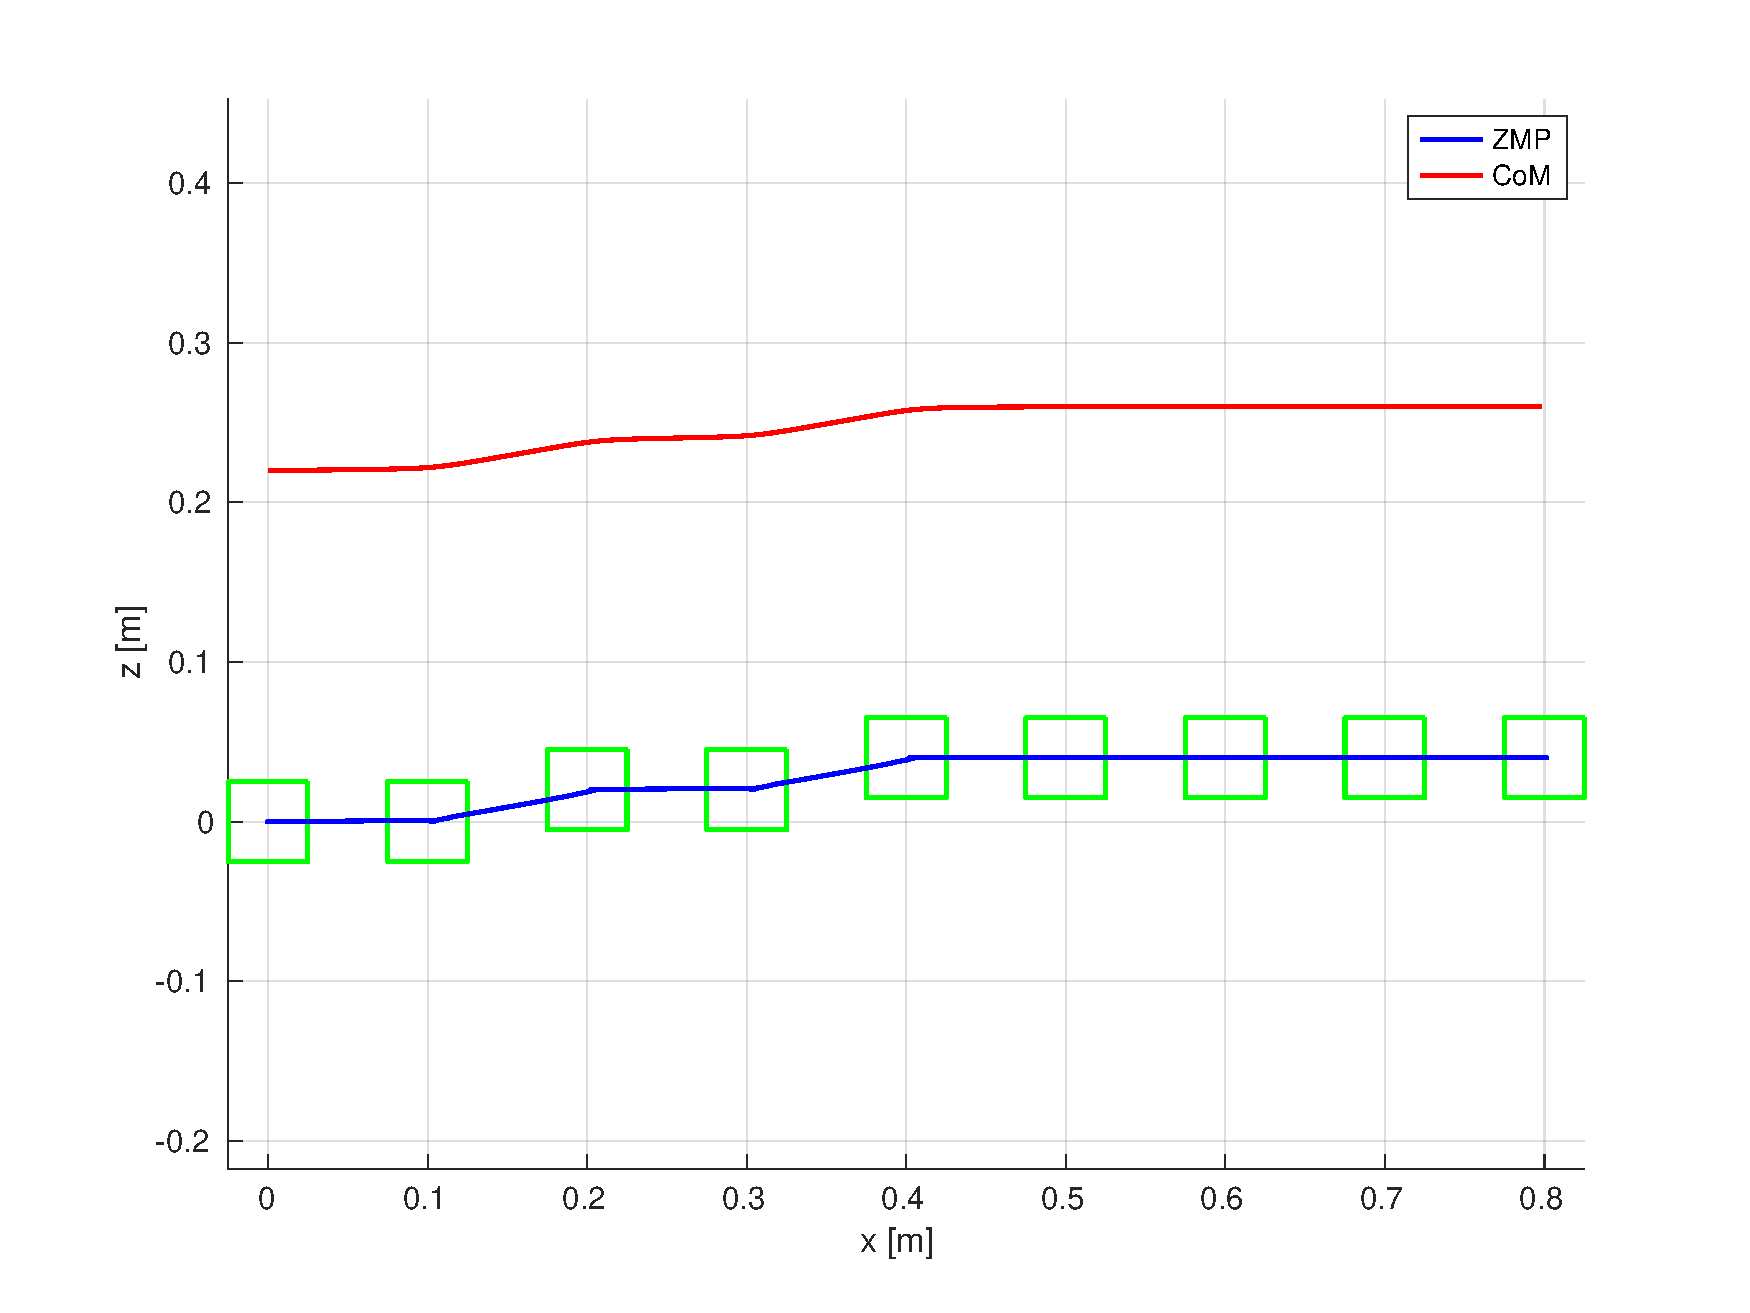
\includegraphics[width=\textwidth]
      {figures/experiments/multiple-staircases/upstairs/xz-plot-2cm.pdf}
  \caption{The plots show how the CoM and the ZMP vary with respect to the
		footsteps in the scenario ``Multiple Staircases (Upstairs)''.
    The green boxes represent the footsteps.}
  \label{fig:experiments:multiple-staircases:upstairs:comzmp}
\end{figure}

\subsection{Downstairs}
The following scenario is called ``Multiple Staircases (Downstairs)'' and it 
consists in making NAO climb a stairway composed of two consecutive staircases 
of 2 cm by moving downstairs. Fig.
\ref{fig:experiments:multiple-staircases:downstairs:videoframes} shows the 
behaviour of the robot for this setting. NAO correctly completes the assigned 
task reaching ground level. Fig. 
\ref{fig:experiments:multiple-staircases:downstairs:comzmp} show how the CoM and 
the ZMP changes through time during this experiment.
\begin{figure}
  \begin{subfigure}{0.48\textwidth}
    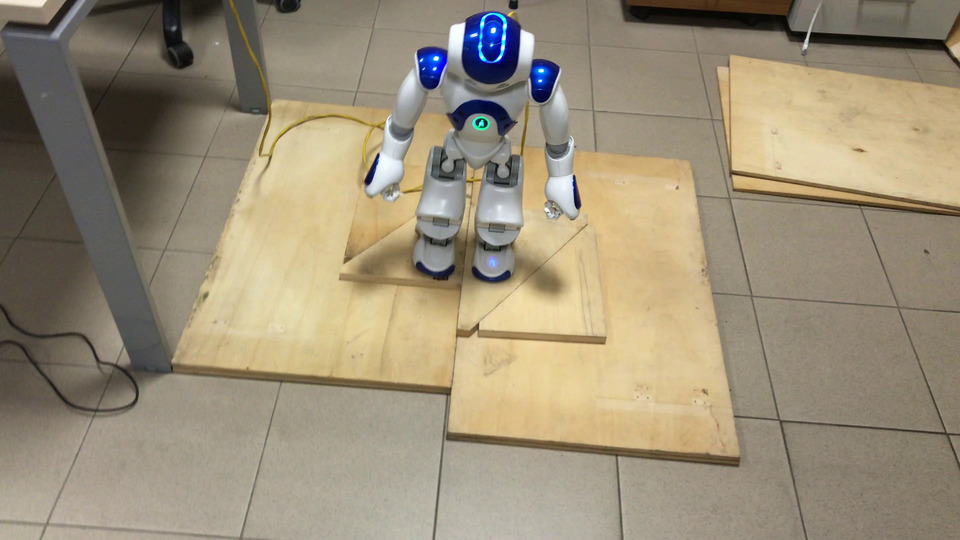
\includegraphics[width=\linewidth]
      {figures/experiments/multiple-staircases/downstairs/video/01.png}
    \caption{Starting position}
    \label{fig:exp:ms:down:frame1}
  \end{subfigure}\hspace*{\fill}
  \begin{subfigure}{0.48\textwidth}
    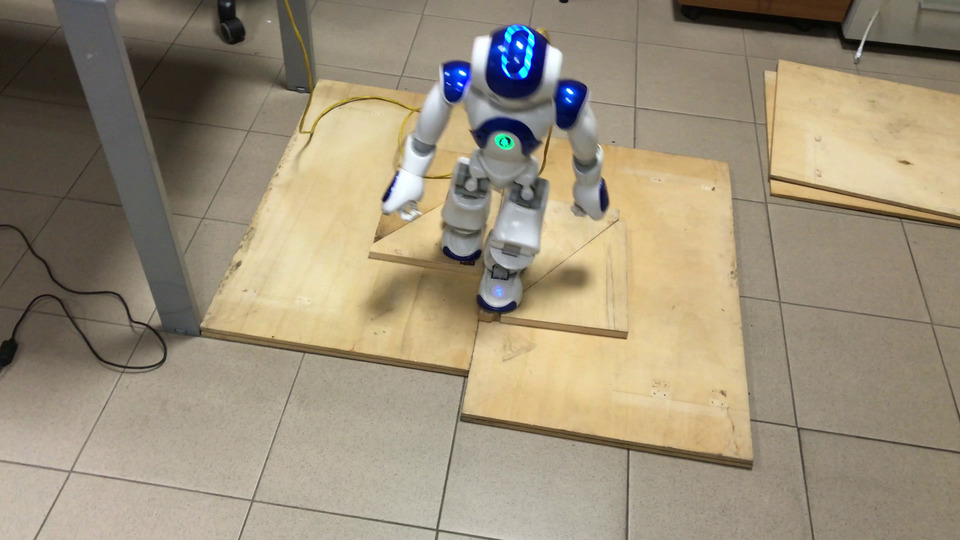
\includegraphics[width=\linewidth]
      {figures/experiments/multiple-staircases/downstairs/video/02.png}
    \caption{First step}
  \end{subfigure}
  \begin{subfigure}{0.48\textwidth}
    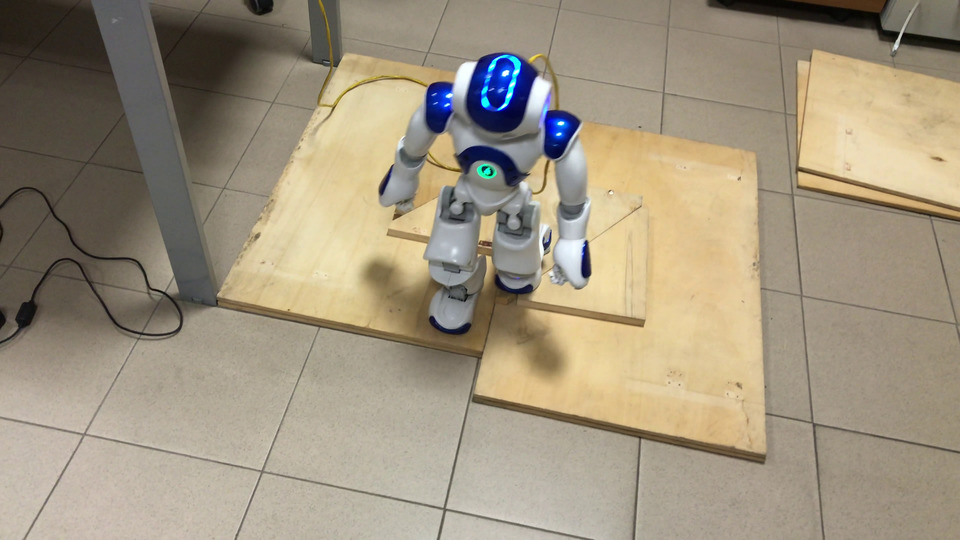
\includegraphics[width=\linewidth]
      {figures/experiments/multiple-staircases/downstairs/video/03.png}
    \caption{Second step}
  \end{subfigure}\hspace*{\fill}
  \begin{subfigure}{0.48\textwidth}
    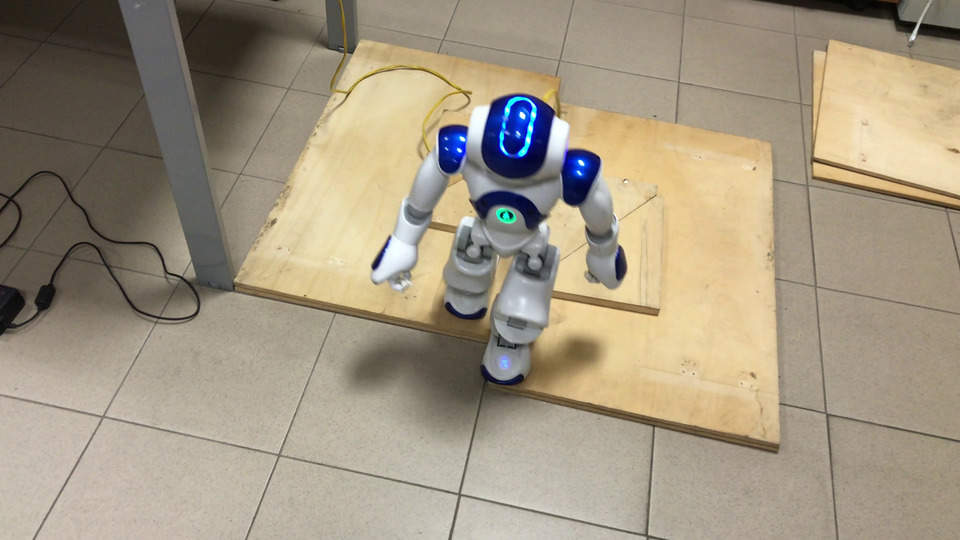
\includegraphics[width=\linewidth]
      {figures/experiments/multiple-staircases/downstairs/video/04.png}
    \caption{Third step}
  \end{subfigure}
  \begin{subfigure}{0.48\textwidth}
    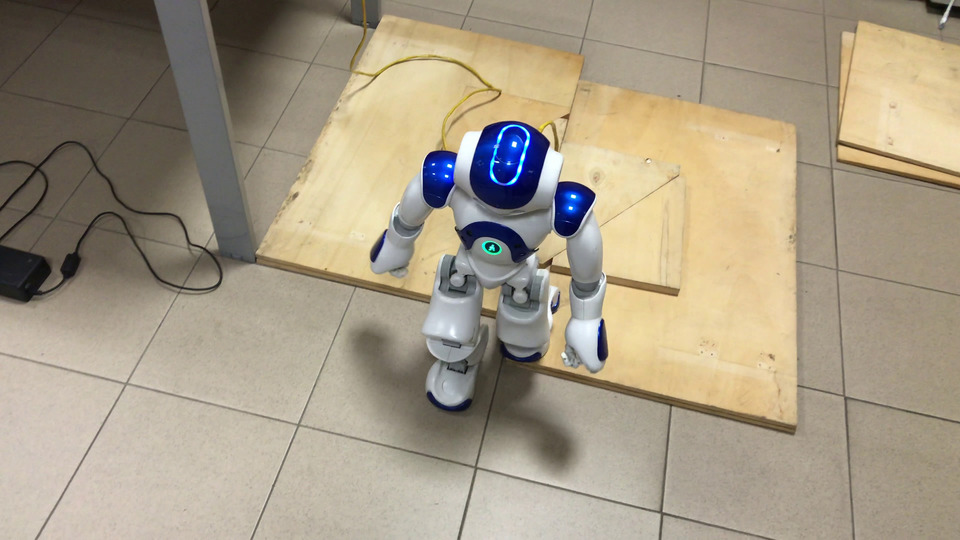
\includegraphics[width=\linewidth]
      {figures/experiments/multiple-staircases/downstairs/video/05.png}
    \caption{Fourth step}
  \end{subfigure}\hspace*{\fill}
  \begin{subfigure}{0.48\textwidth}
    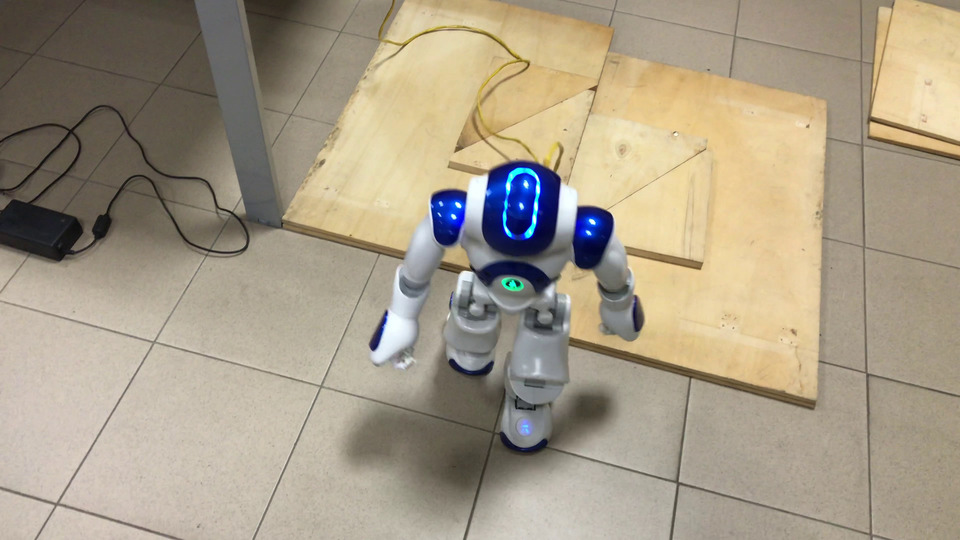
\includegraphics[width=\linewidth]
      {figures/experiments/multiple-staircases/downstairs/video/06.png}
    \caption{Fifth step}
  \end{subfigure}
  \caption{The figures show the motion of the robot for the scenario
      ``Multiple Staircases (Downstairs)''. The robot starts on top of the 
      stairway (Fig. \ref{fig:exp:ms:down:frame1}), then it places 
      each step one in front of the other without colliding with the staircases,
      safely reaching ground level. Each staircase has a height of 2 cm.}
  \label{fig:experiments:multiple-staircases:downstairs:videoframes}
\end{figure}

\begin{figure}
  \centering
  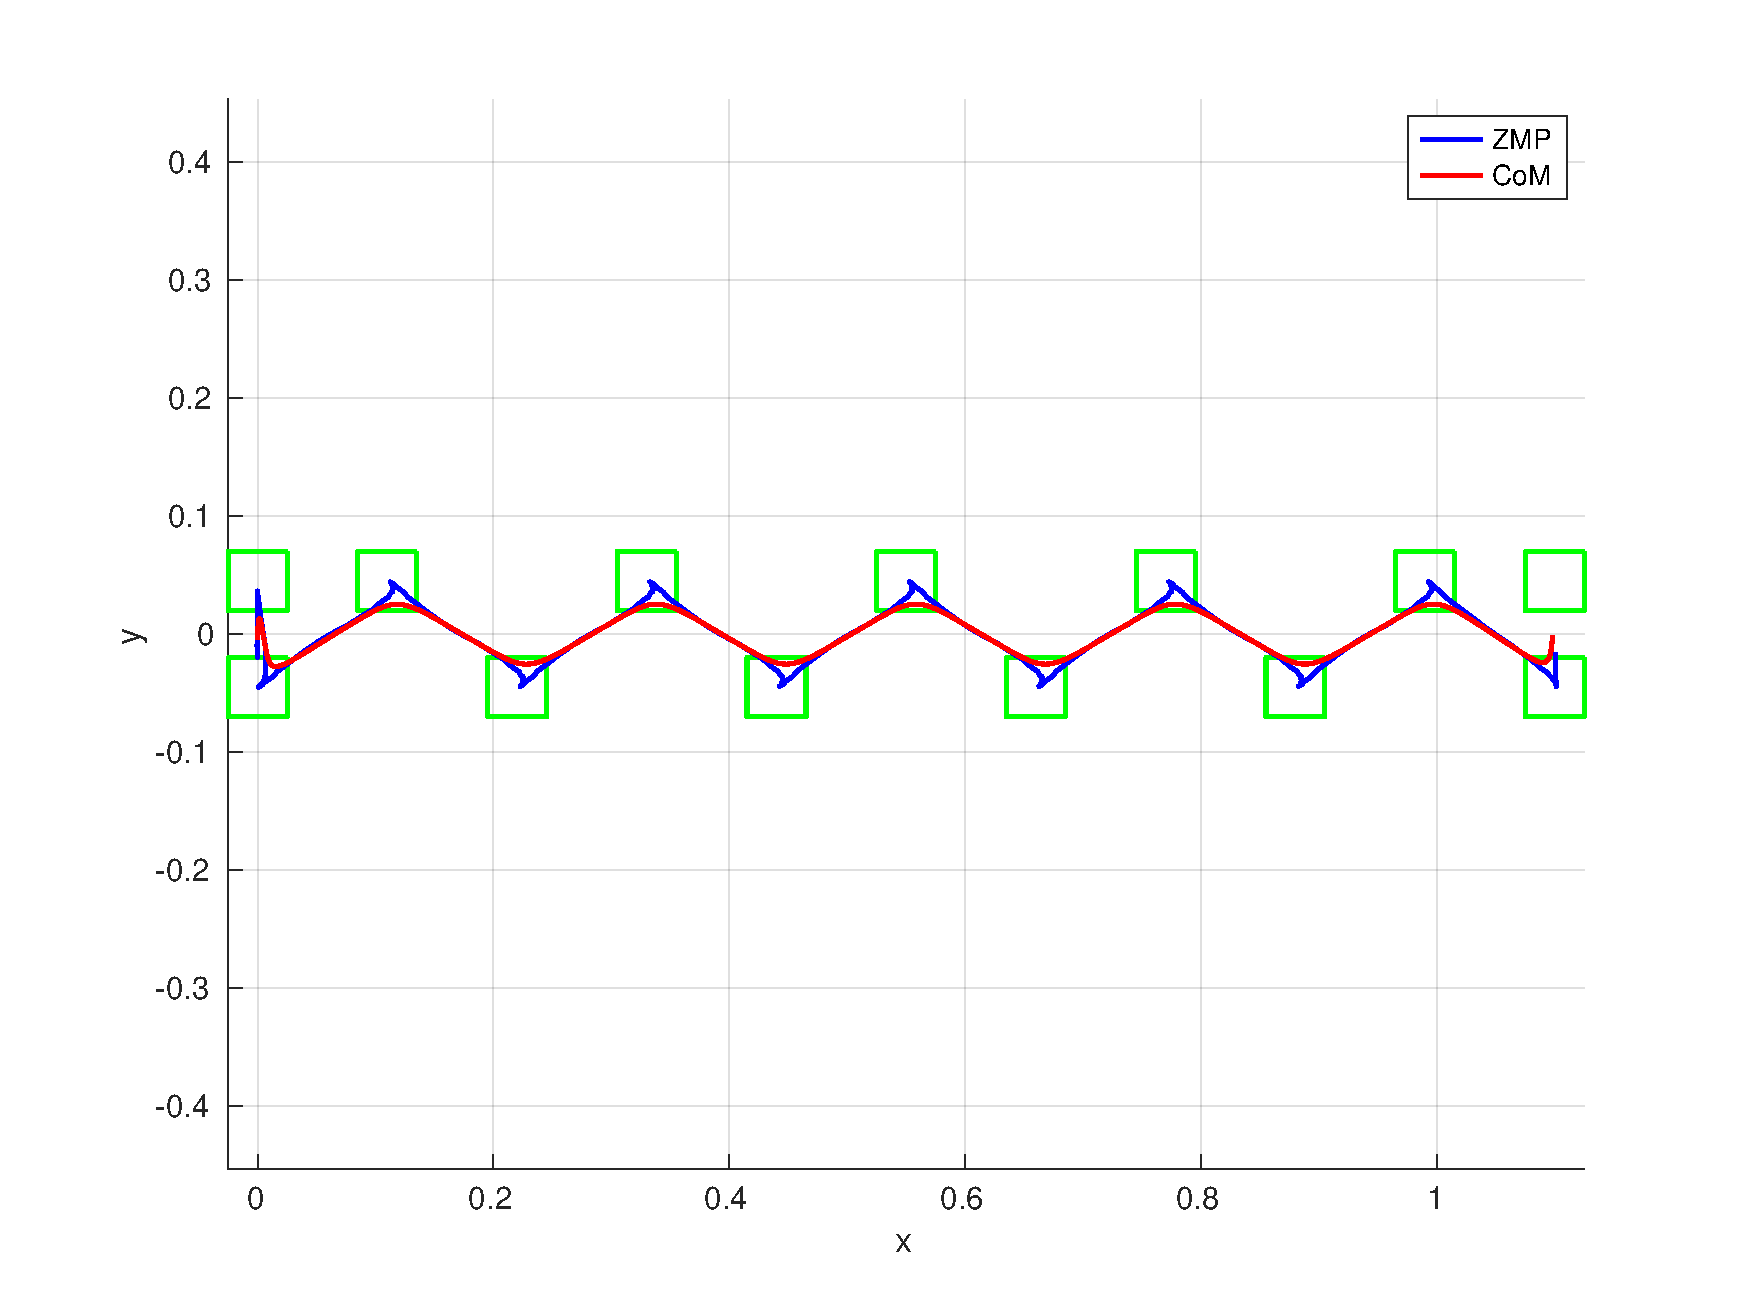
\includegraphics[width=\textwidth]
      {figures/experiments/multiple-staircases/downstairs/xy-plot-2cm.pdf}
  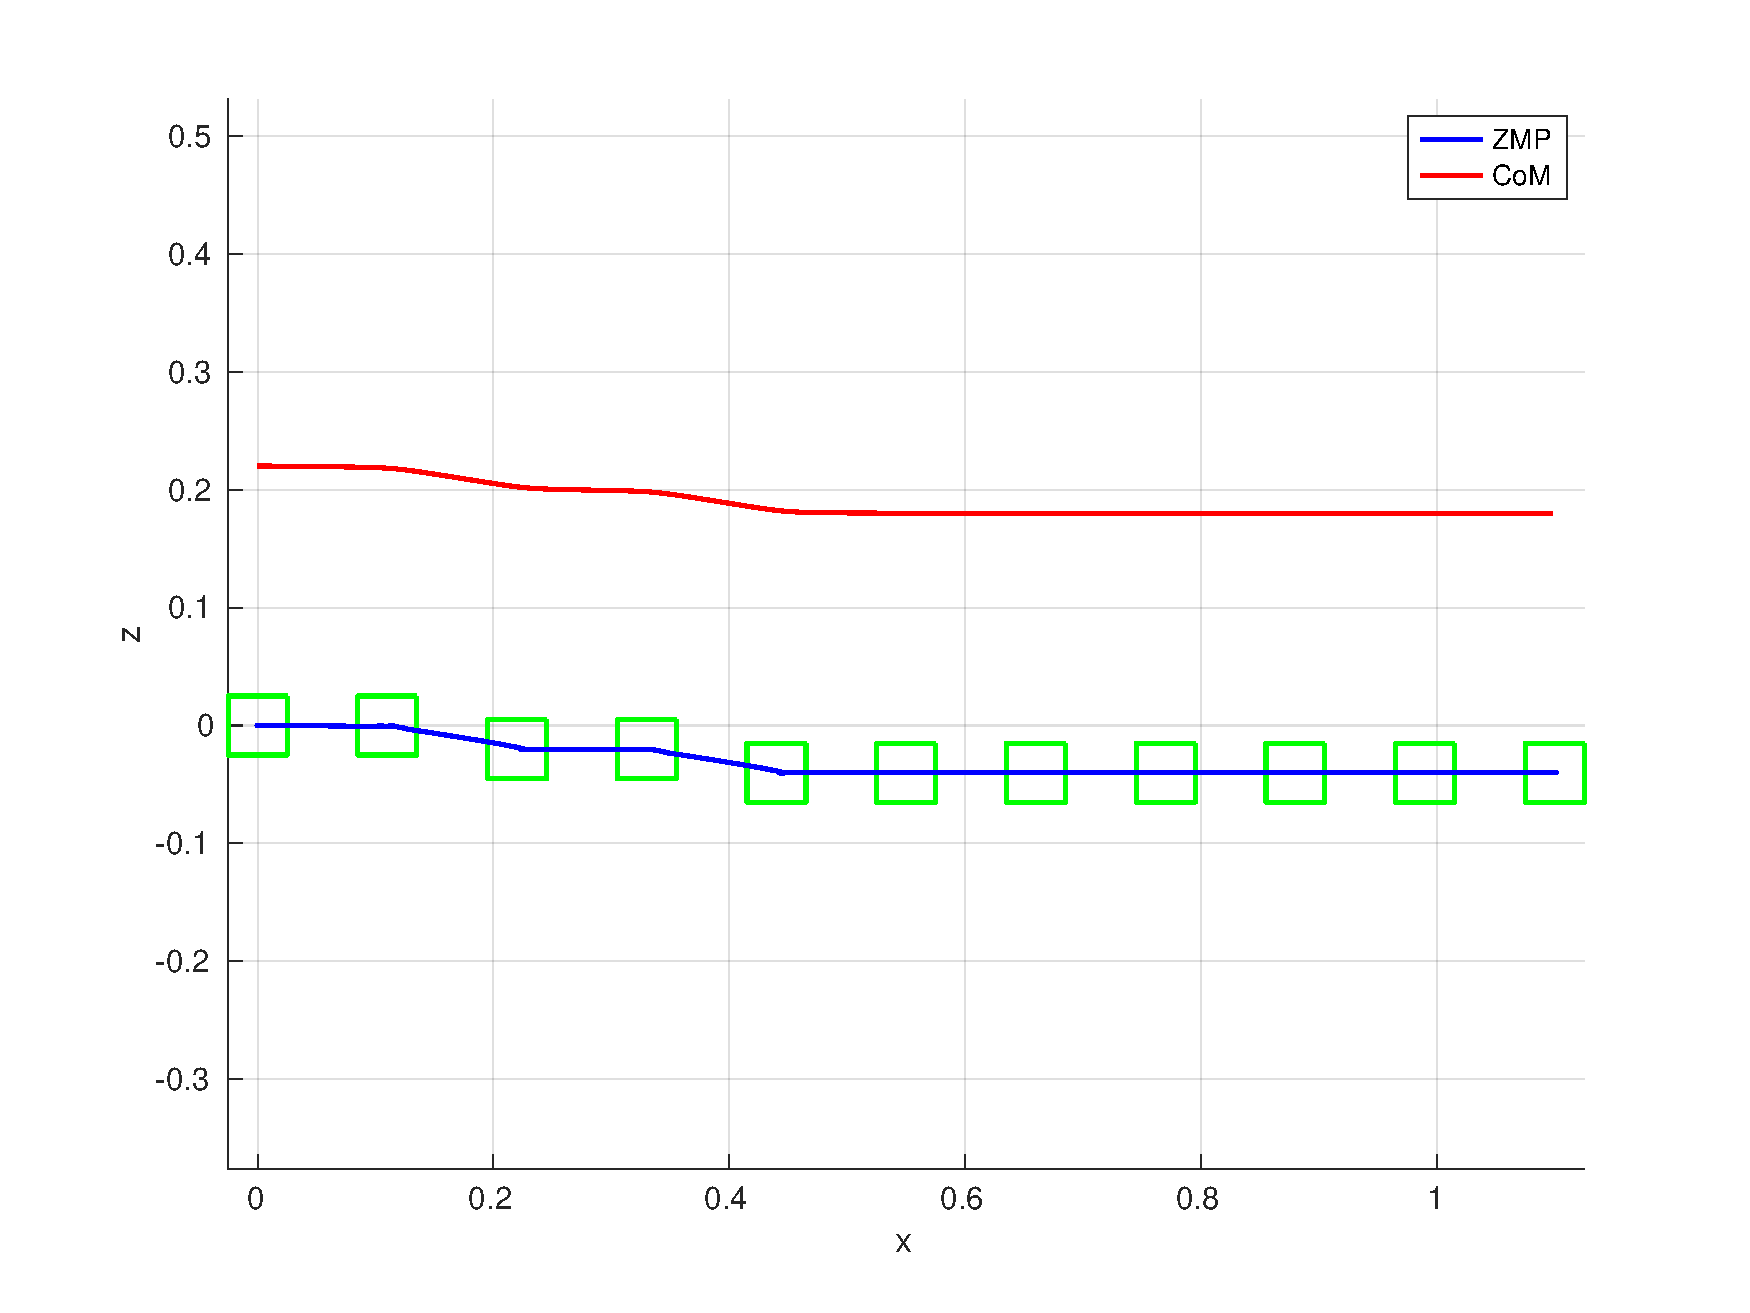
\includegraphics[width=\textwidth]
      {figures/experiments/multiple-staircases/downstairs/xz-plot-2cm.pdf}
  \caption{The plots show how the CoM and the ZMP vary with respect to the
		footsteps in the scenario ``Multiple Staircases (Downstairs)''.
    The green boxes represent the footsteps.}
  \label{fig:experiments:multiple-staircases:downstairs:comzmp}
\end{figure}

\section{Obstacle Avoidance}
The third experiment introduces the footstep planner described in Chapter
\ref{ch:rrt-based-footstep-planning} into 
the project. The aim is to test the behaviour of the planner in a simple 
\textit{World of Stairs} scenario that contains a platform put between the
initial position of the robot and the goal region that can not be climbed by 
NAO. The goal of the footstep planner is those of finding a feasible 
plan not just avoiding the obstacle, but also by not stepping onto it. 
The robot would, in fact, not climb it correctly because of its
physical limitations.
The elevation map used in this experiment has been manually generated.

The planner generates a plan of 31 steps (Fig.
\ref{fig:experiments:obstacle-avoidance:footstep-plan}) in 70 ms
(Table \ref{table:rrt-stats}). The 
corresponding tree in shown in Fig. 
\ref{fig:experiments:obstacle-avoidance:rrt-tree} and it has size 488.
Fig. \ref{fig:experiments:obstacle-avoidance:videoframes} shows the robot
moving inside the environment from its initial position 
to the goal region (a circle of radius 10 cm 
with center at the position of the ball).

Since the planner 
is based on RRT, the generated plan is not optimal. It is, in fact,
possible to notice how the robot does not move fluidly, sometimes putting 
the foot back and forth before changing position. This is a
characteristic of RRT that could be changed by building the algorithm on top
of RRT* \cite{rrtstar}.
\begin{figure}
  \begin{subfigure}{0.48\textwidth}
    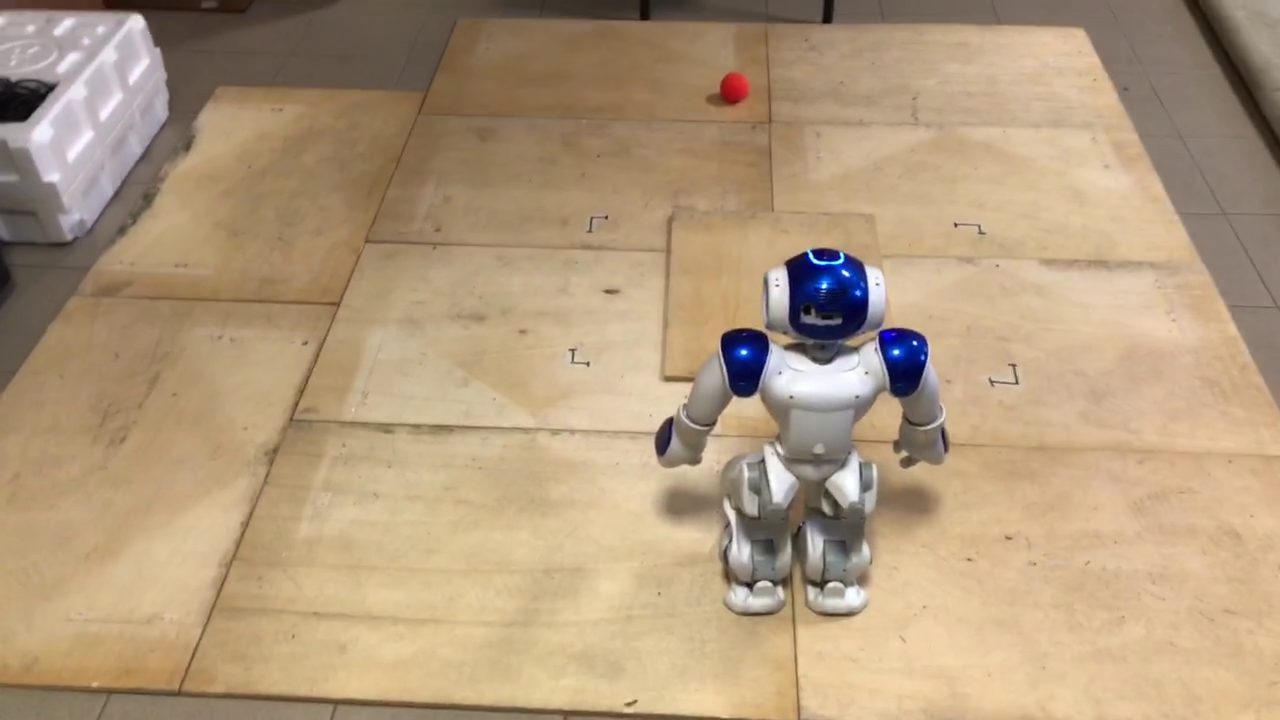
\includegraphics[width=\linewidth]
      {figures/experiments/obstacle-avoidance/video/01.png}
    \caption{Starting position}
    \label{fig:exp:obs:frame1}
  \end{subfigure}\hspace*{\fill}
  \begin{subfigure}{0.48\textwidth}
    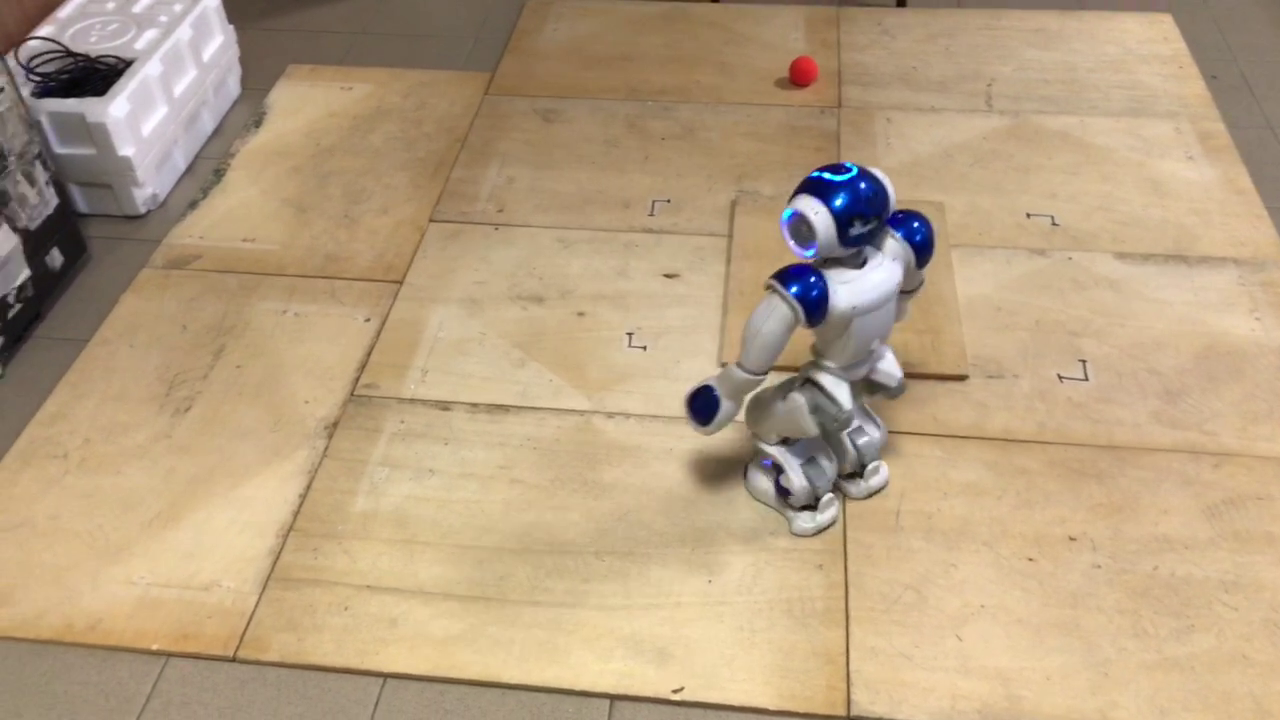
\includegraphics[width=\linewidth]
      {figures/experiments/obstacle-avoidance/video/02.png}
    \caption{Moving to the left}
    \label{fig:exp:obs:frame2}
  \end{subfigure}
  \begin{subfigure}{0.48\textwidth}
    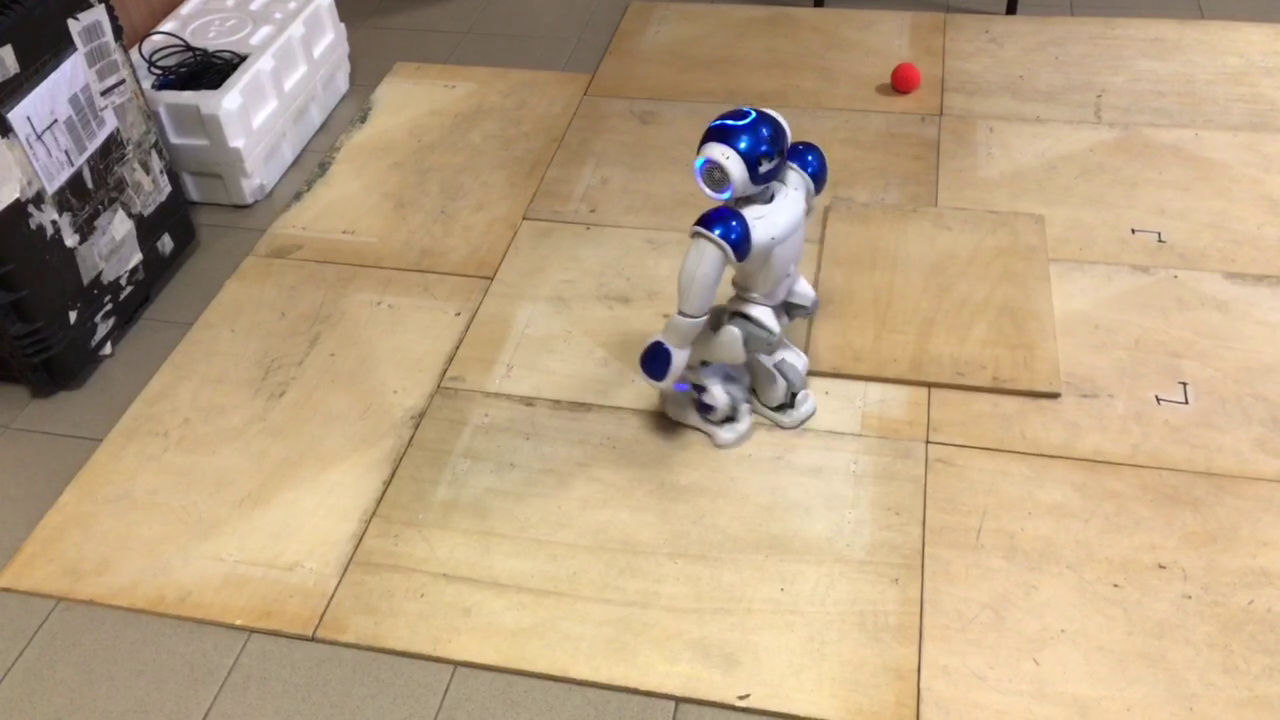
\includegraphics[width=\linewidth]
      {figures/experiments/obstacle-avoidance/video/03.png}
    \caption{Avoiding the obstacle}
  \end{subfigure}\hspace*{\fill}
  \begin{subfigure}{0.48\textwidth}
    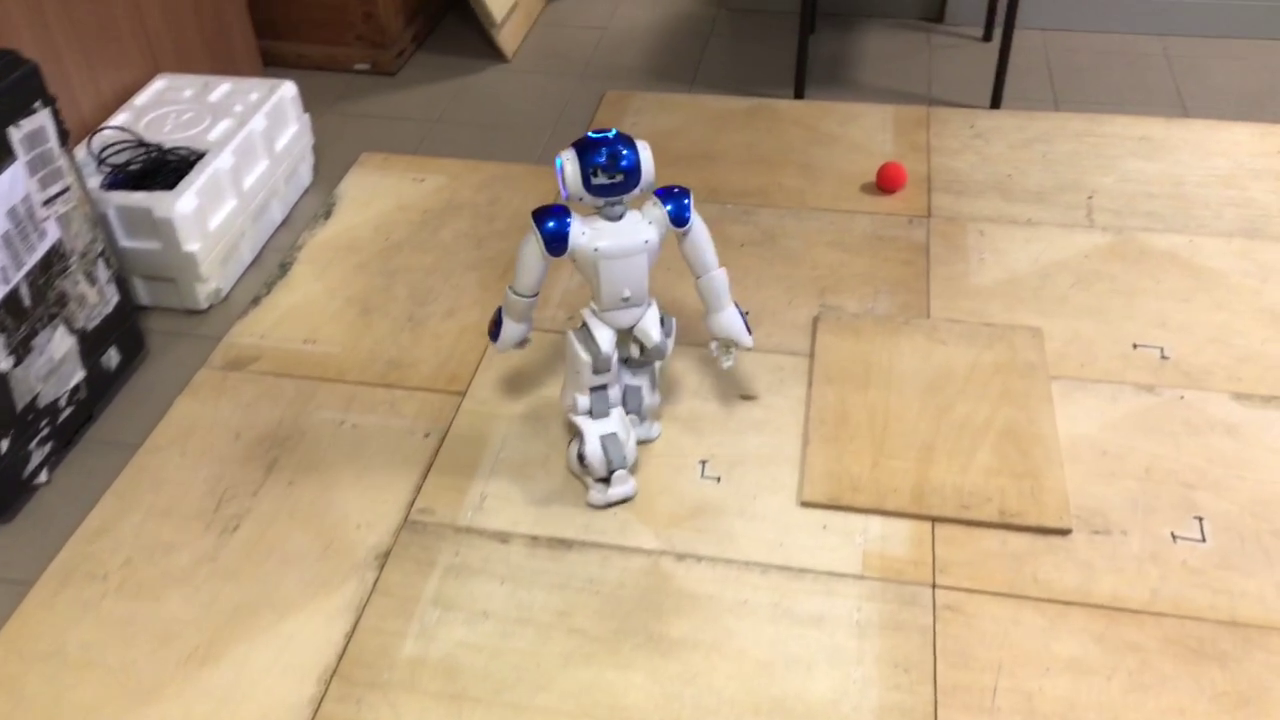
\includegraphics[width=\linewidth]
      {figures/experiments/obstacle-avoidance/video/04.png}
    \caption{Moving forward}
  \end{subfigure}
  \begin{subfigure}{0.48\textwidth}
    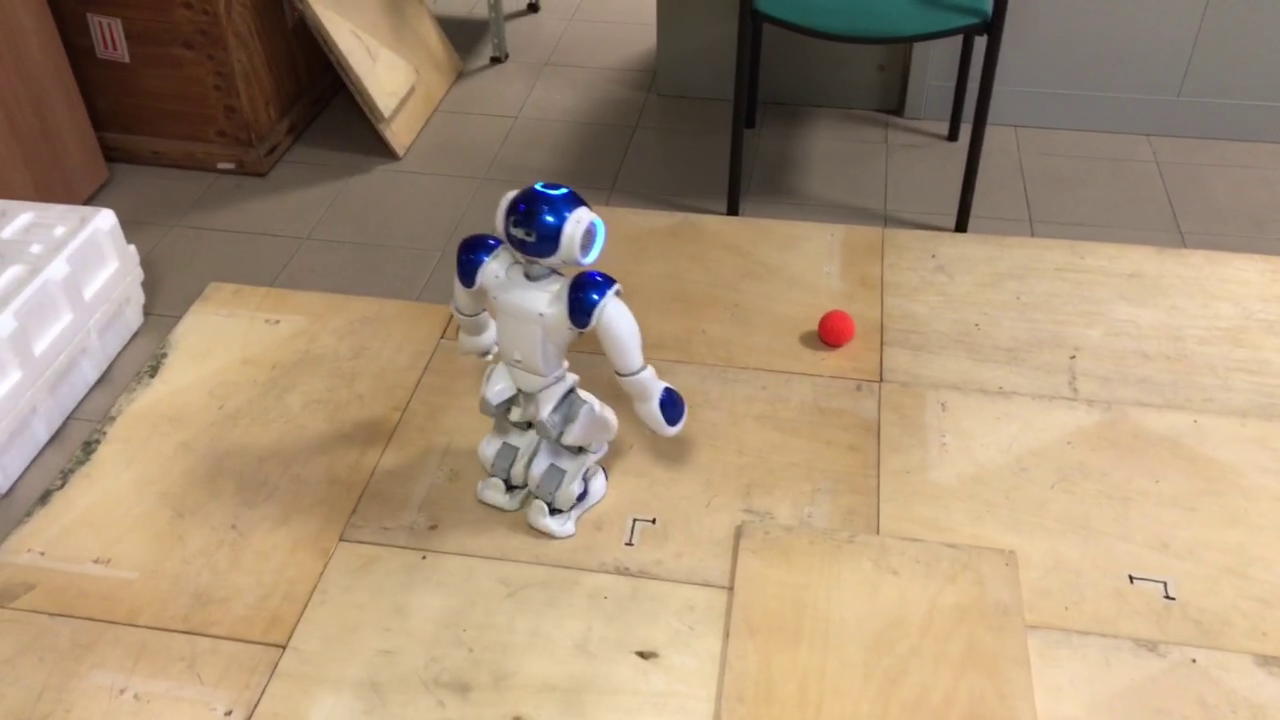
\includegraphics[width=\linewidth]
      {figures/experiments/obstacle-avoidance/video/05.png}
    \caption{Moving towards the goal}
    \label{fig:exp:obs:frame5}
  \end{subfigure}\hspace*{\fill}
  \begin{subfigure}{0.48\textwidth}
    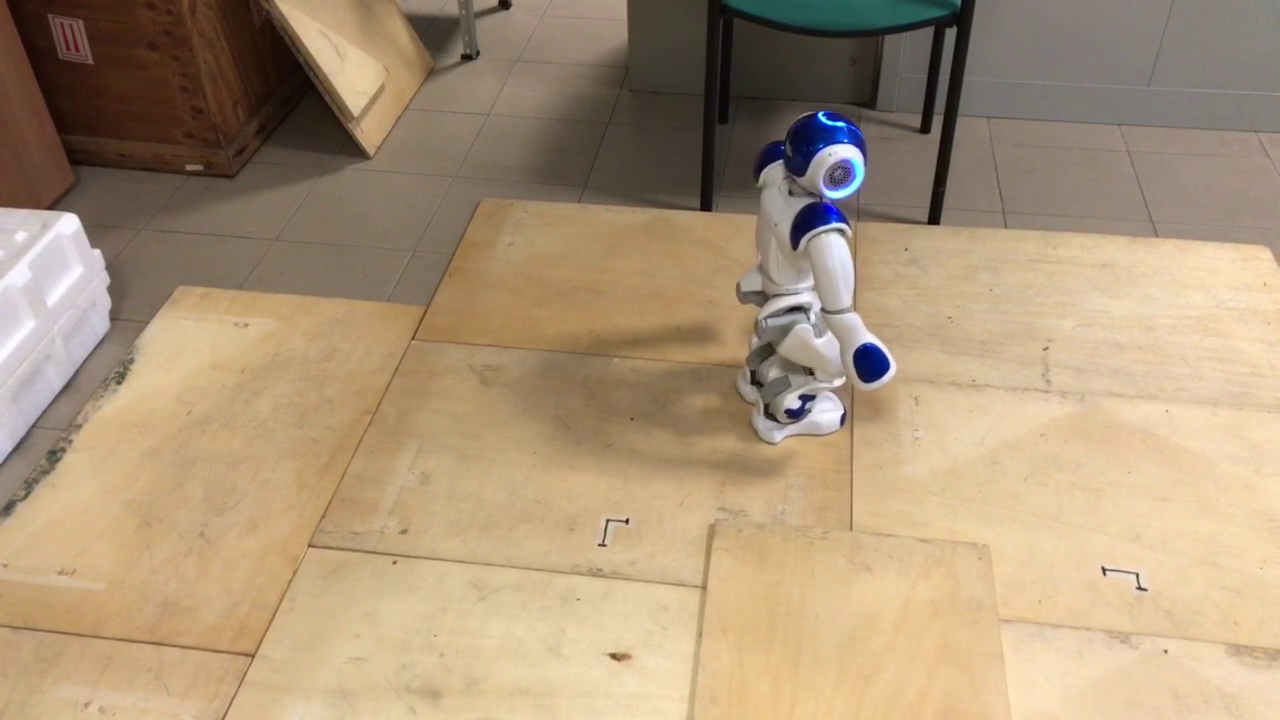
\includegraphics[width=\linewidth]
      {figures/experiments/obstacle-avoidance/video/06.png}
    \caption{Goal region reached}
    \label{fig:exp:obs:frame6}
  \end{subfigure}
  \caption{The figures show the motion of the robot for the scenario
      ``Obstacle Avoidance''. The robot starts in front of the obstacle
      (Fig. \ref{fig:exp:obs:frame1}), then it moves to its left correctly
      avoiding it (Fig. \ref{fig:exp:obs:frame2}-\ref{fig:exp:obs:frame5})
      until it reaches the goal region (Fig. \ref{fig:exp:obs:frame6}),
      whose center is represented by 
      the ball. The goal region is a circle with a radius of 10 cm. 
      Note that even if the obstacle has a height of 2 cm, NAO can not climb it 
      because of its kinematic limitations, hence, the planner takes
      into account the mechanical capabilities of the robot, generating a 
      safe and realizable footstep plan.}
  \label{fig:experiments:obstacle-avoidance:videoframes}
\end{figure}

\begin{figure}
    \centering
    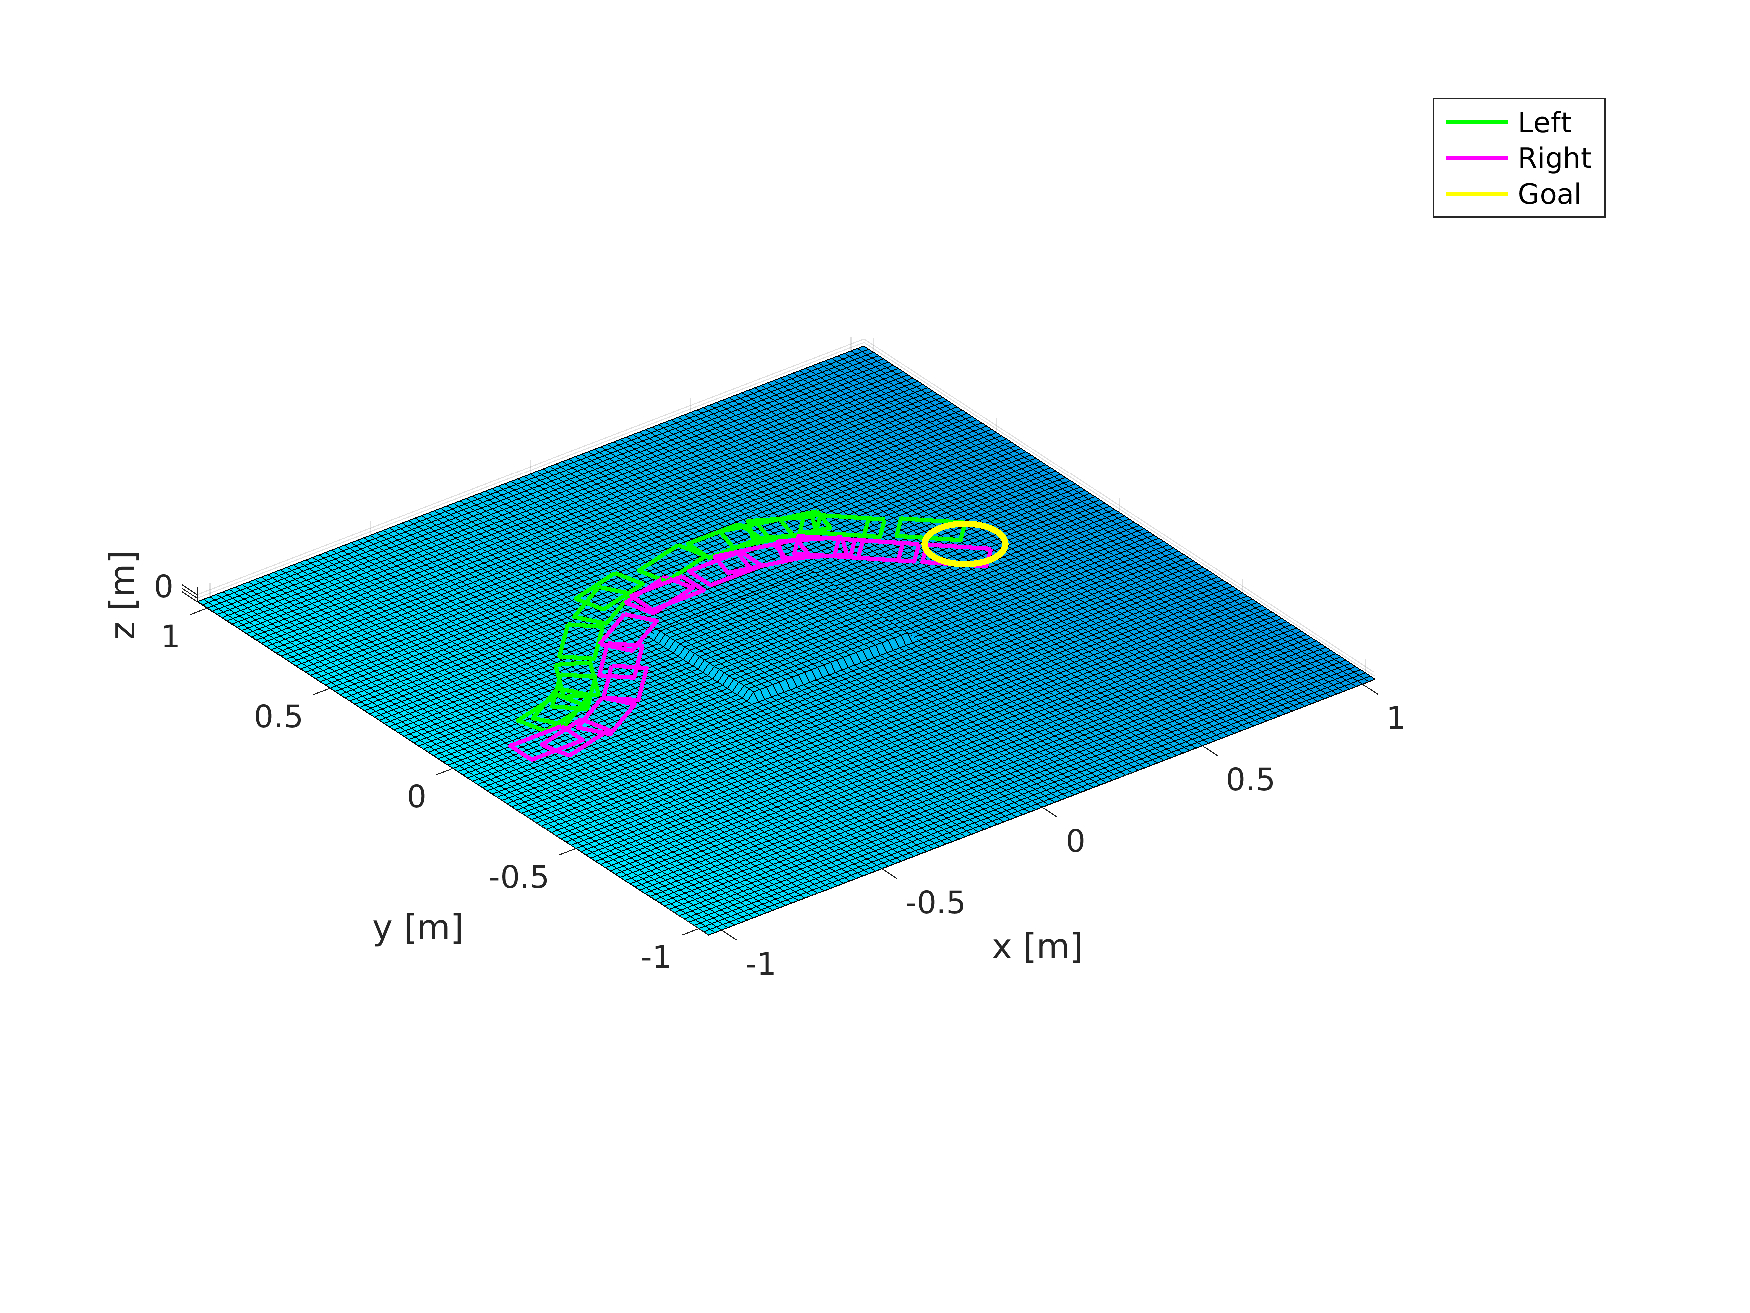
\includegraphics[width=0.95\textwidth]
        {figures/experiments/obstacle-avoidance/footstep-plan.pdf}
    \caption{Footstep plan generated for the scenario ``Obstacle Avoidance''.}
    \label{fig:experiments:obstacle-avoidance:footstep-plan}
\end{figure}
\begin{figure}
    \centering
    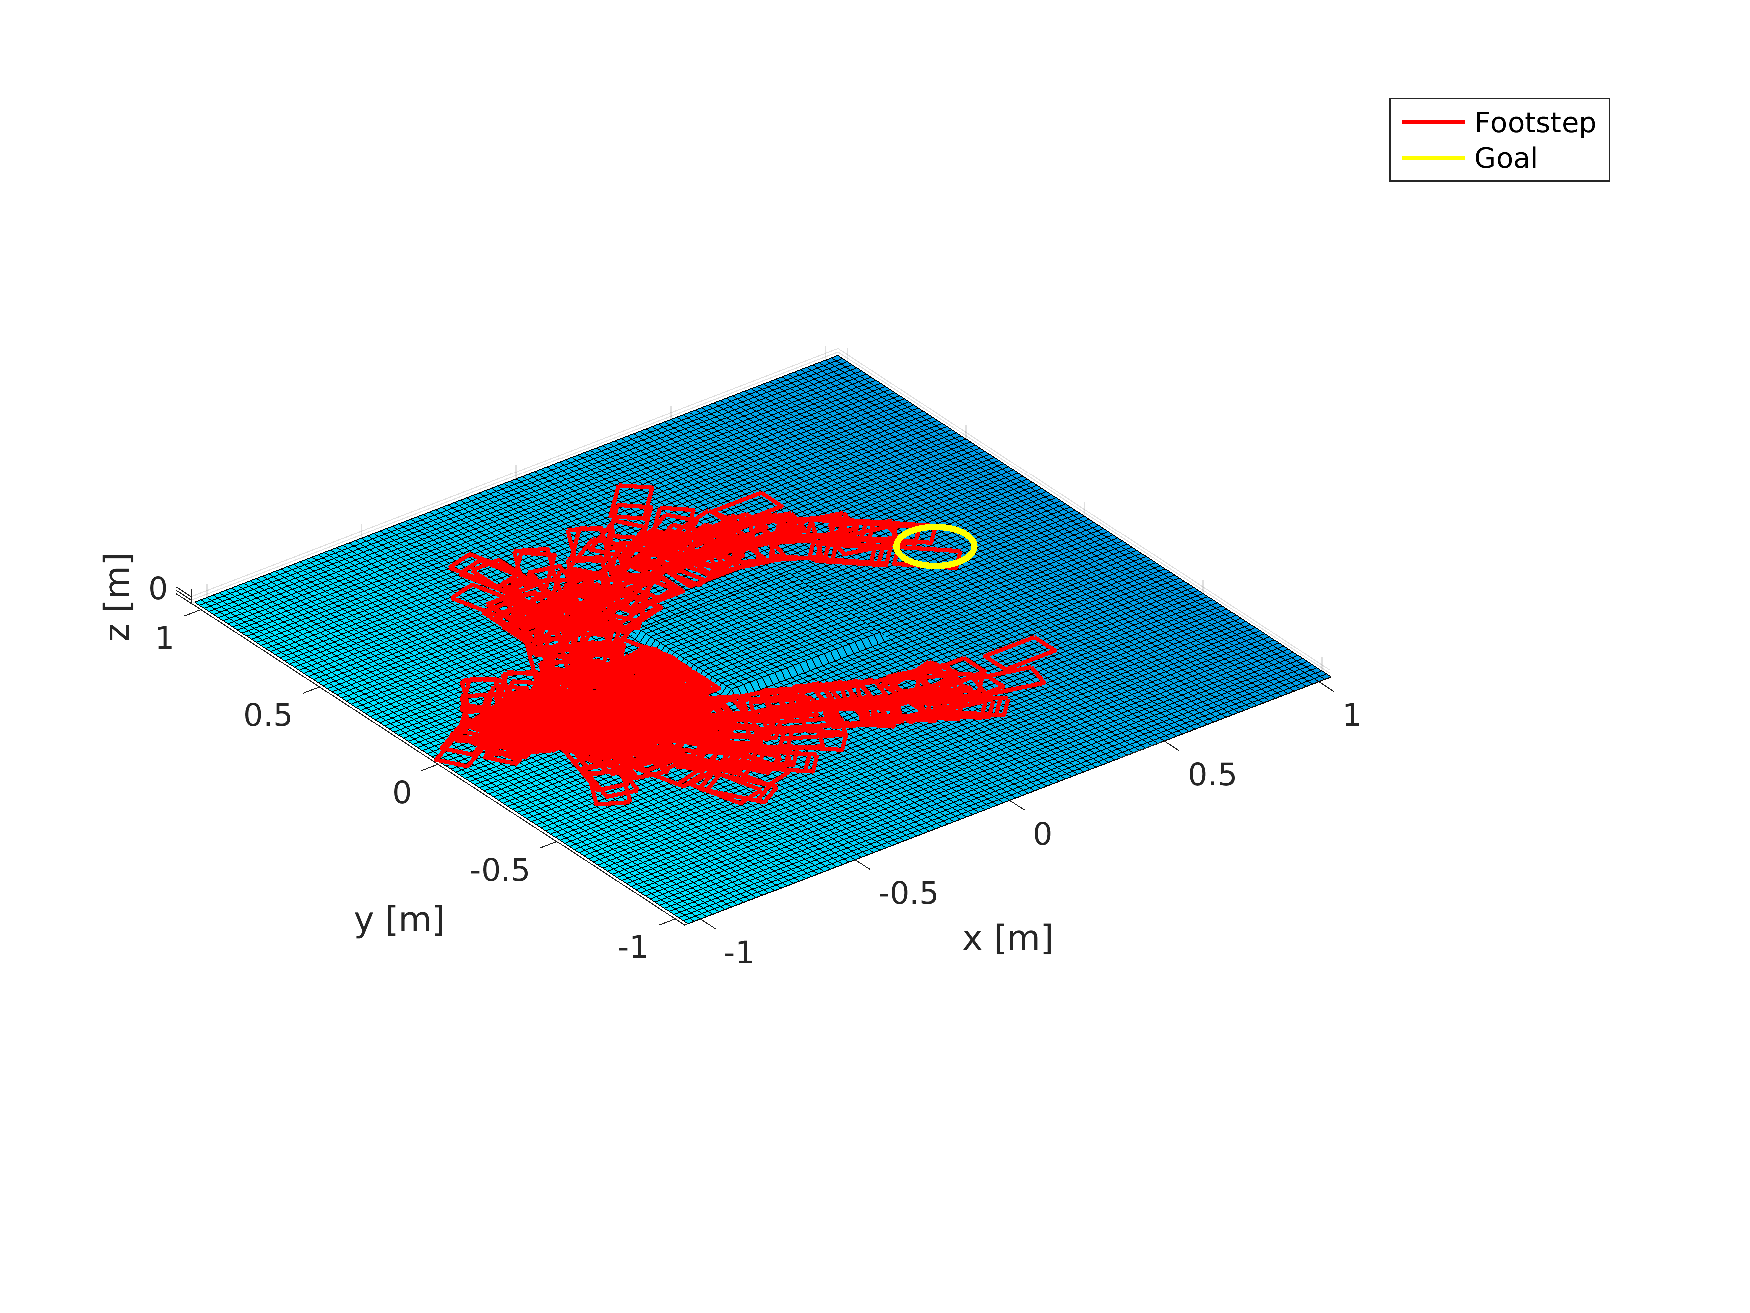
\includegraphics[width=0.95\textwidth]
        {figures/experiments/obstacle-avoidance/rrt-tree.pdf}
    \caption{Tree generated for the scenario ``Obstacle Avoidance''.}
    \label{fig:experiments:obstacle-avoidance:rrt-tree}
\end{figure}

\section{Stair Climbing in Unknown Environment}
\label{sec:stair-climbing-unkenv}
The last experiment introduces \texttt{elevation\_mapping} (Chapter 
\ref{ch:elevation-map-generation}) into the project. The aim is to test the 
behaviour of the framework in an unknown \textit{World of Stairs} environment.
The idea is to generate a map autonomously exploiting the depth sensor of the 
ASUS Xtion Pro camera, which has been put on top of NAO humanoid robot.
The generated map is sent to the footstep planner described in Chapter 
\ref{ch:rrt-based-footstep-planning} which is in charge of generating a 
plan that brings the robot to a predefined goal region. This goal region is 
placed on top of a stairway, so that the robot must climb the stairs in order 
to complete the task. The generation of the map has been already described in 
Chapter \ref{ch:elevation-map-generation} and it is shown in Fig. 
\ref{fig:onlymap-xtion-20cm}. As already discussed, once the footstep plan 
is generated, it is sent to the robot which executes a proper motion 
using the Variable Height CoM IS-MPC (Chapter \ref{ch:vh-com-is-mpc}).

The planner generates a plan of 10 steps (Fig.
\ref{fig:experiments:unknown-env:footstep-plan}) in 0.331s (Table
\ref{table:rrt-stats}). Note that the runtime of this experiment is slower
than the previous one because of the noise contained in the elevation map, 
which causes the planner to discard many configurations since they do not
satisfy requirement R2 of the footstep planner
(Chapter \ref{ch:rrt-based-footstep-planning}). In this experiment the 
requirement R2 has been relaxed allowing a maximum difference of 7 mm between
the $z$ coordinate of the footstep and the height of a cell in the map.
The corresponding 
tree is shown in Fig. \ref{fig:experiments:unknown-env:rrt-tree} and it has 
size 454. Fig. \ref{fig:experiments:unkenv:videoframes} shows the robot moving
inside the environment from its initial position
to the goal region (a circle of radius 10 cm with center at the position
of the ball).

\begin{table}
	\centering
	\begin{tabular}{*{5}{c}}
    Scenario & Tree Size & Solution Size & Runtime\\
		\hline
    Obtacle Avoidance & 488 & 31 & 70 ms \\
    Stair Climbing in Unknown Environment & 454 & 10 & 331 ms
	\end{tabular}
  \caption{Performances of the planner on different scenarios. Note that
	    even if the size of the trees are similar, the runtime of ``Stair
			Climbing in Unknown Environment'' is slower due to noise in the 
			elevation map. All the 
      experiment have been performed on an Intel Core i5-5257U @ 2.70 Ghz.}
	\label{table:rrt-stats}
\end{table}

\begin{figure}
  \begin{subfigure}{0.48\textwidth}
    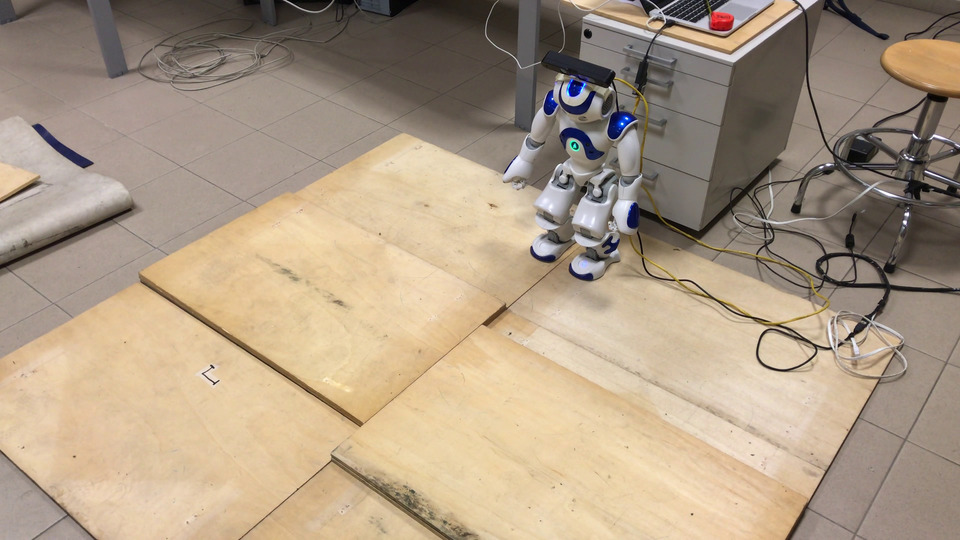
\includegraphics[width=\linewidth]
      {figures/experiments/unknown-env/video/01.png}
    \caption{Starting position}
    \label{fig:exp:unkenv:frame1}
  \end{subfigure}\hspace*{\fill}
  \begin{subfigure}{0.48\textwidth}
    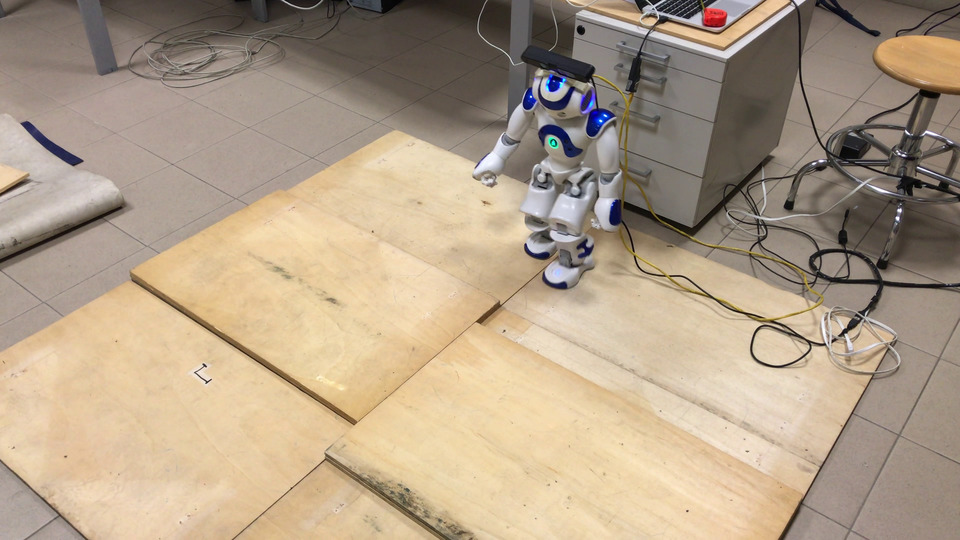
\includegraphics[width=\linewidth]
      {figures/experiments/unknown-env/video/02.png}
    \caption{First step}
    \label{fig:exp:unkenv:frame2}
  \end{subfigure}
  \begin{subfigure}{0.48\textwidth}
    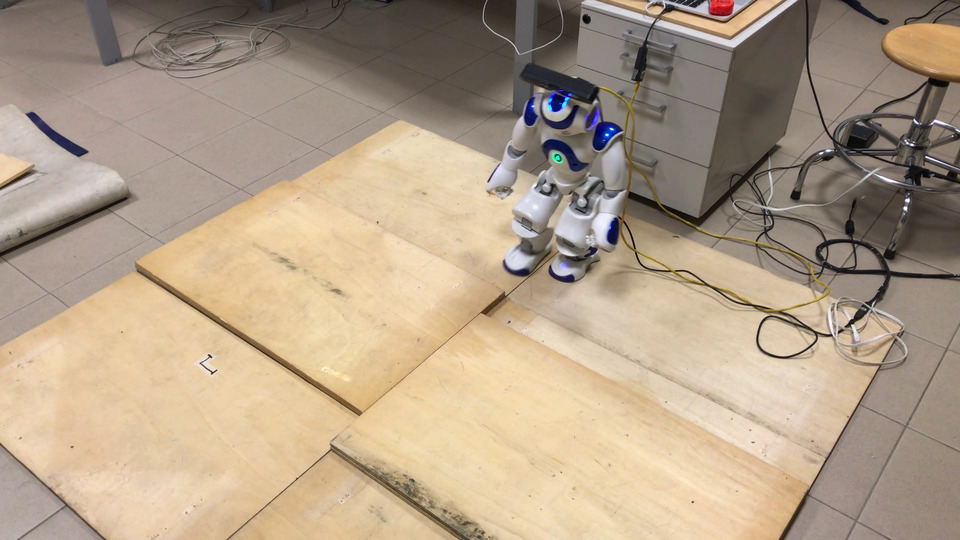
\includegraphics[width=\linewidth]
      {figures/experiments/unknown-env/video/03.png}
    \caption{Second step}
  \end{subfigure}\hspace*{\fill}
  \begin{subfigure}{0.48\textwidth}
    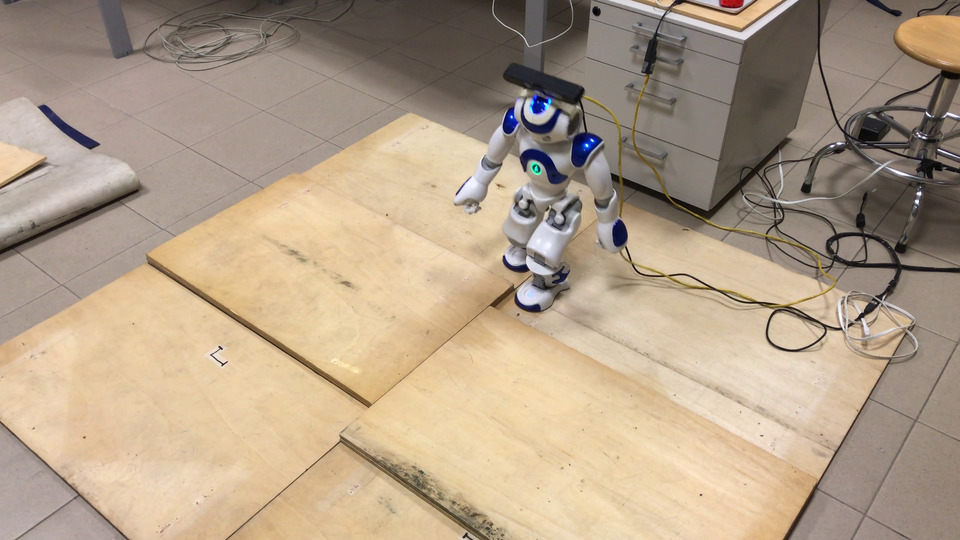
\includegraphics[width=\linewidth]
      {figures/experiments/unknown-env/video/04.png}
    \caption{Third step}
  \end{subfigure}
  \begin{subfigure}{0.48\textwidth}
    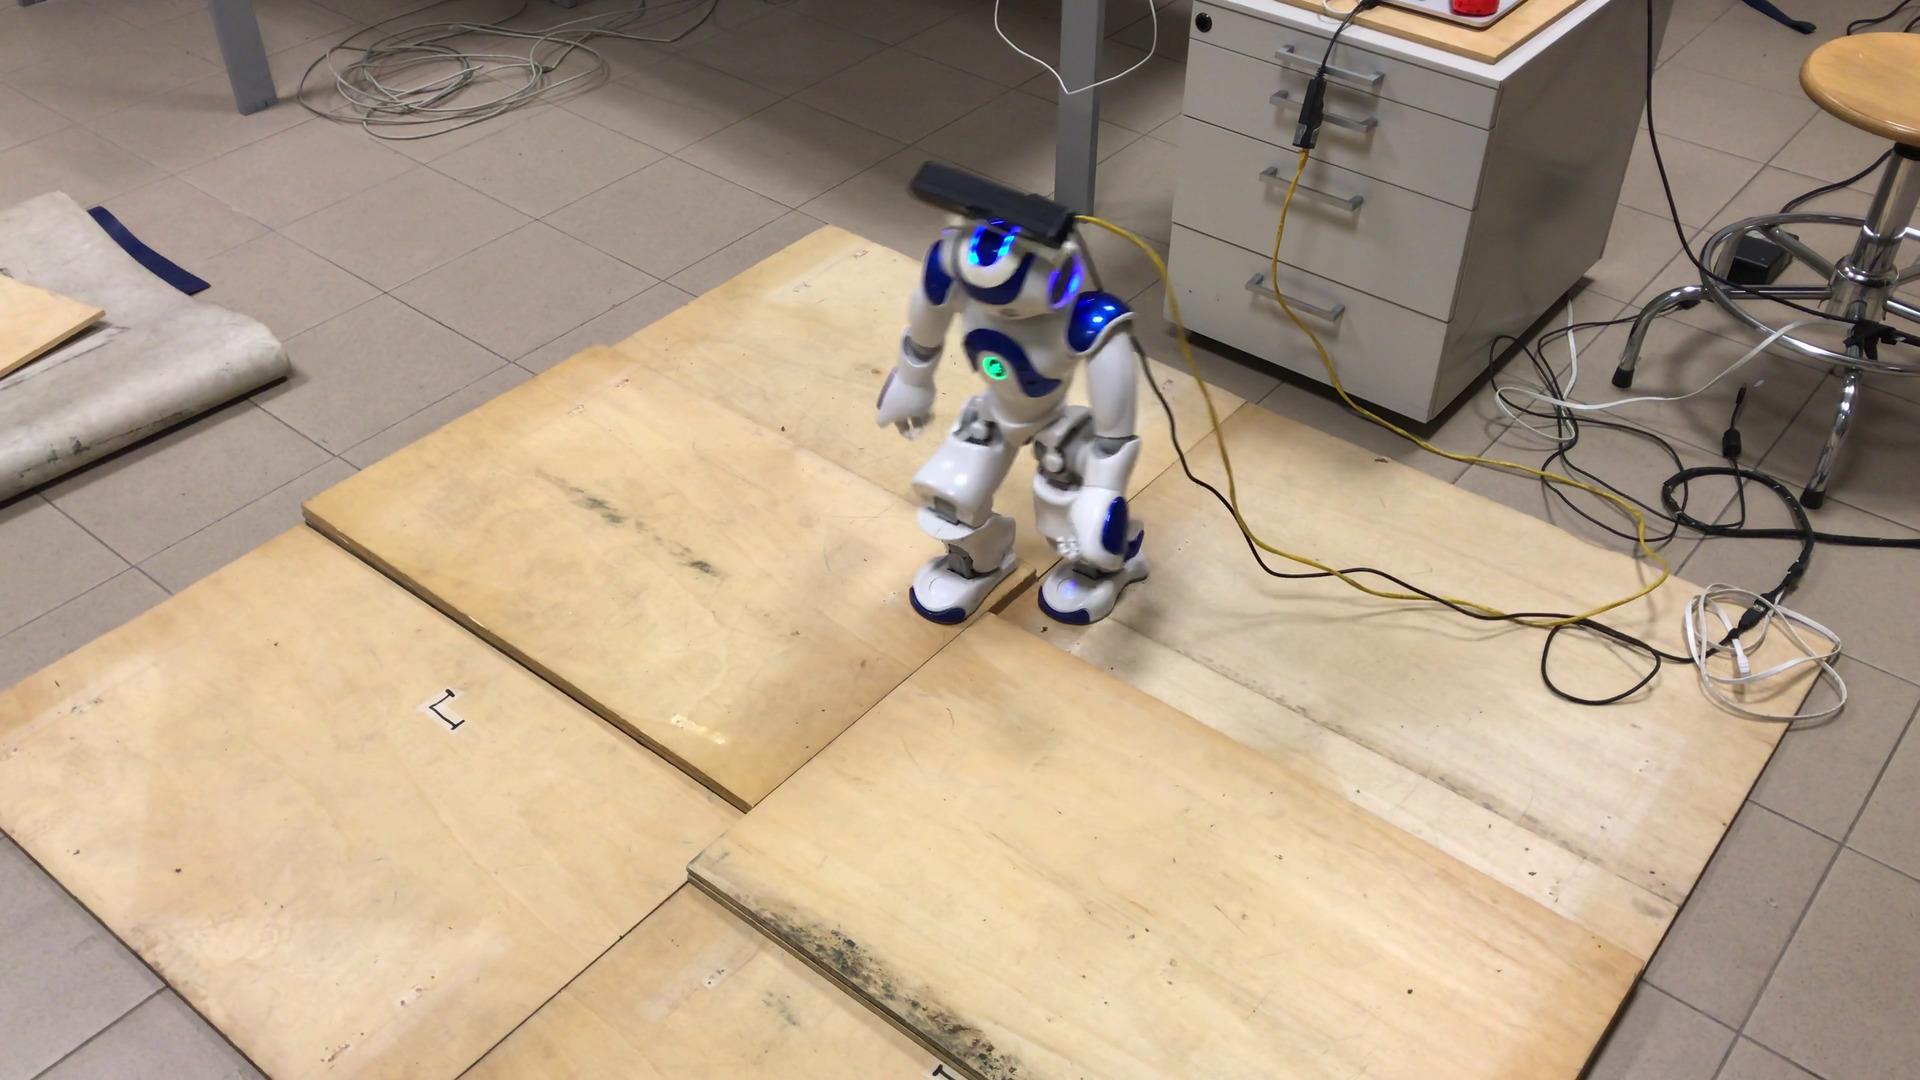
\includegraphics[width=\linewidth]
      {figures/experiments/unknown-env/video/05.png}
    \caption{Fourth step}
  \end{subfigure}\hspace*{\fill}
  \begin{subfigure}{0.48\textwidth}
    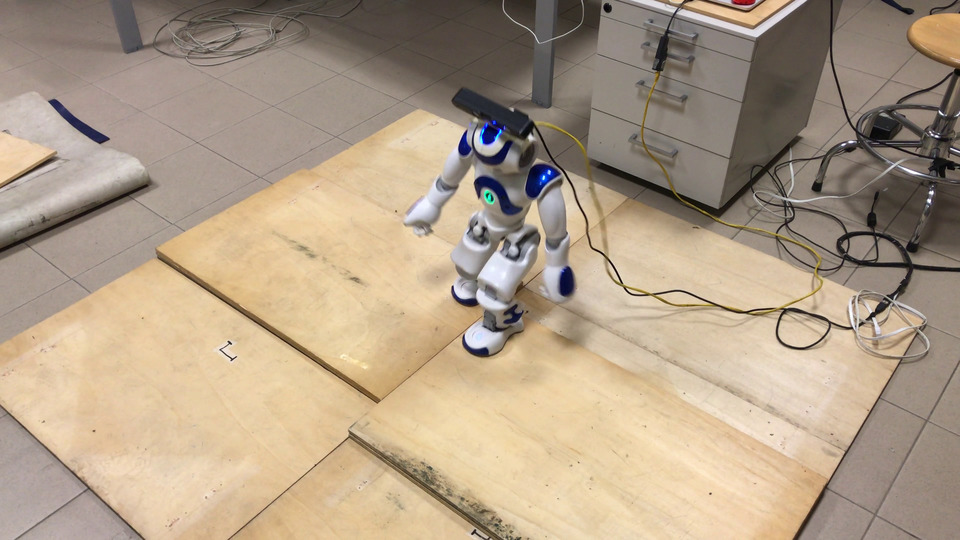
\includegraphics[width=\linewidth]
      {figures/experiments/unknown-env/video/06.png}
    \caption{Fifth step}
  \end{subfigure}
  \begin{subfigure}{0.48\textwidth}
    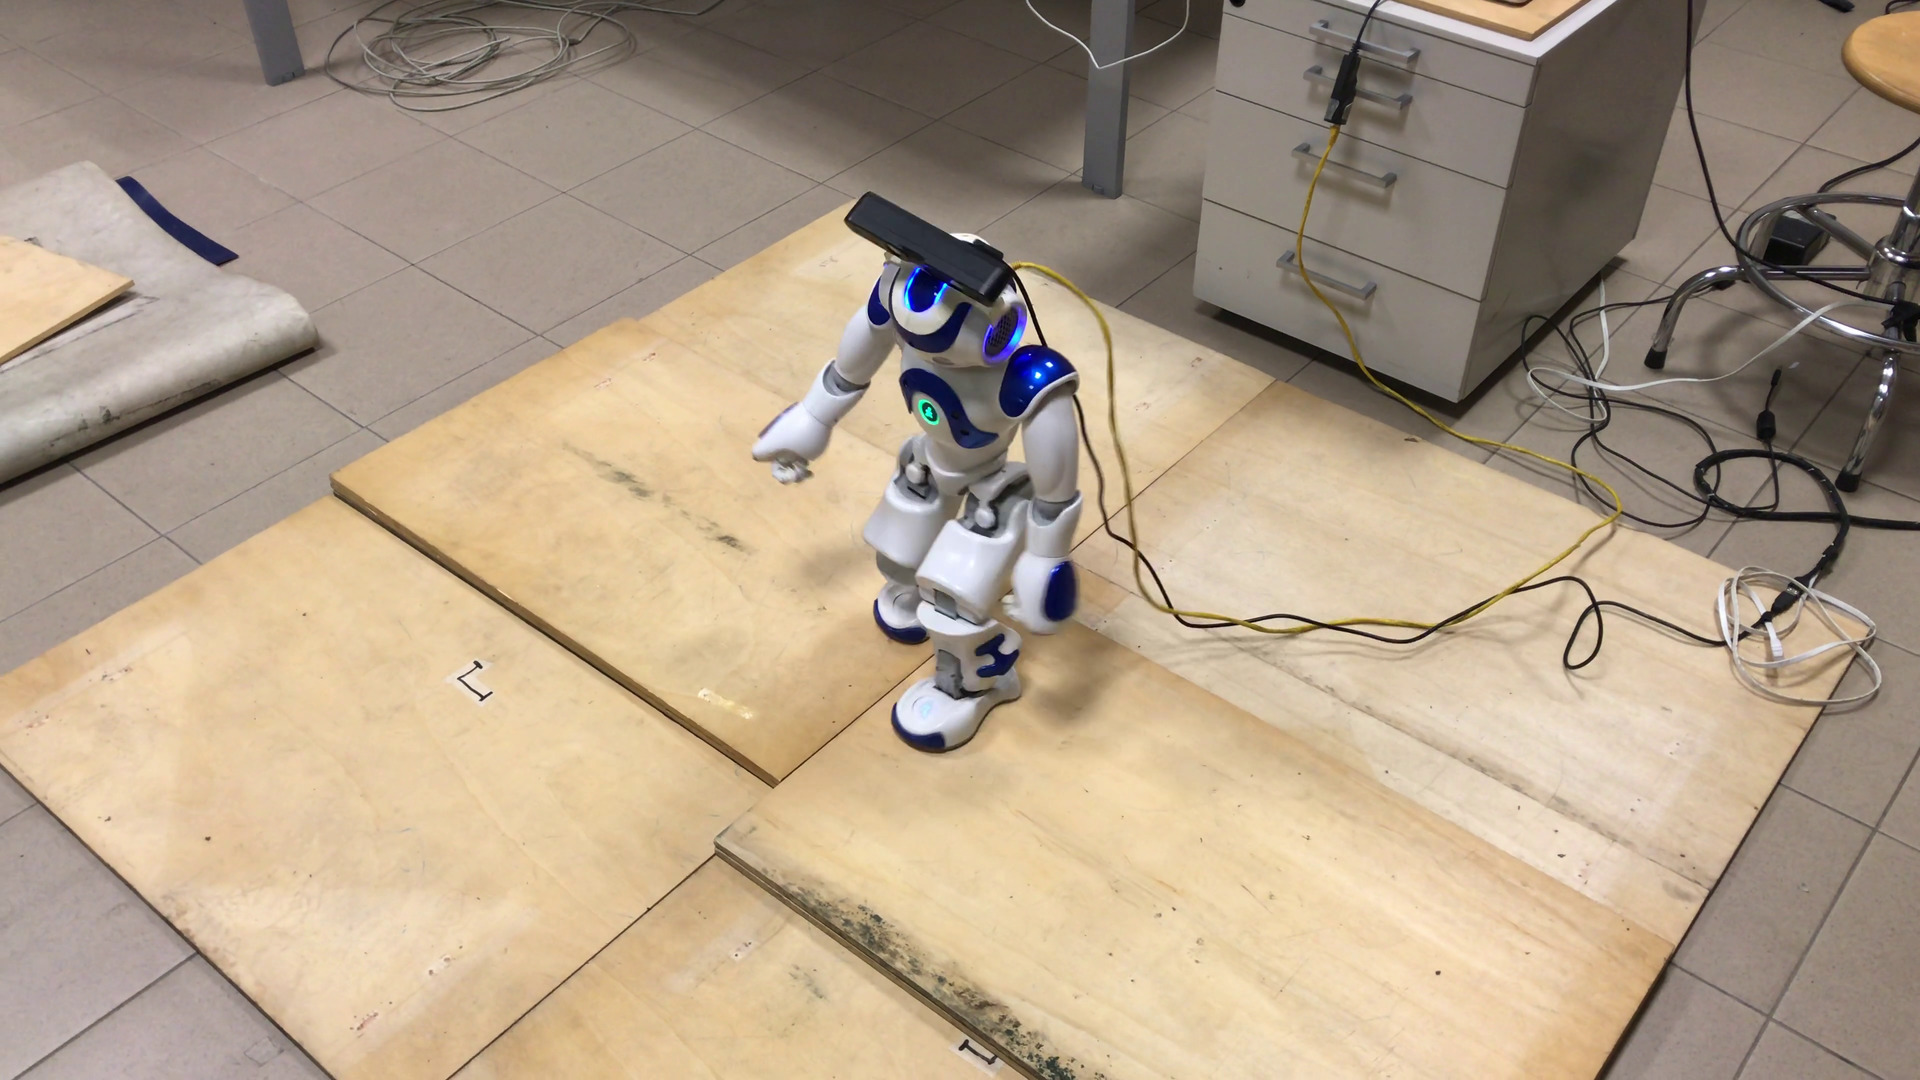
\includegraphics[width=\linewidth]
      {figures/experiments/unknown-env/video/07.png}
    \caption{Seventh step}
  \end{subfigure}\hspace*{\fill}
  \begin{subfigure}{0.48\textwidth}
    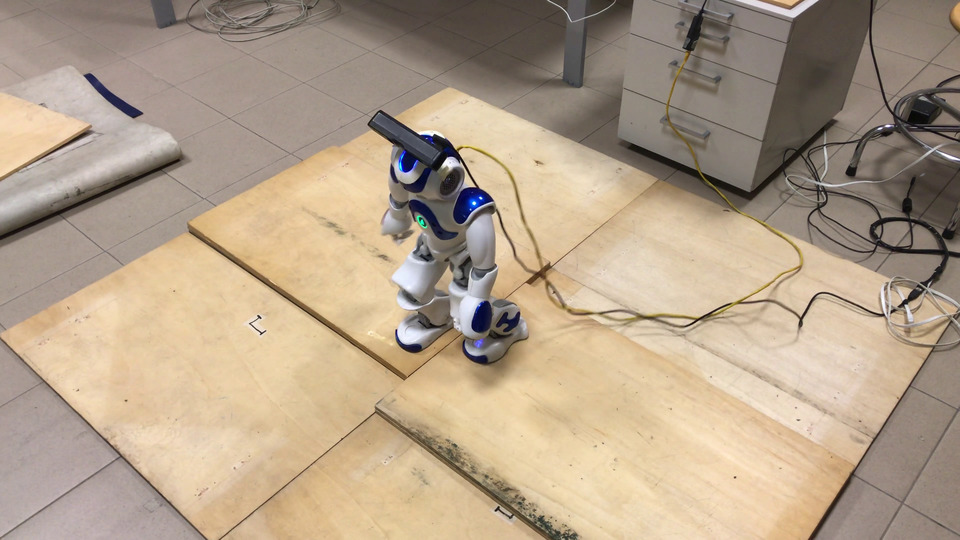
\includegraphics[width=\linewidth]
      {figures/experiments/unknown-env/video/08.png}
    \caption{Eighth step}
  \end{subfigure} \caption{The figures show the motion of the robot
      for the scenario ``Stair Climbing in Unknown Environment''.
      The robot starts at 20 cm 
      from the first staircase (Fig. \ref{fig:exp:unkenv:frame1}). Before 
      starting the motion (Fig. \ref{fig:exp:unkenv:frame2}), an
      elevation map is built by the \texttt{elevation\_mapping} framework
      (Chapter \ref{ch:elevation-map-generation}),
      which receives the depth frames from the ASUS Xtion Pro placed 
      on top of the robot. The elevation map is sent to the planner, which 
      generates a footstep plan (Chapter \ref{ch:rrt-based-footstep-planning}).
      The footstep plan is then sent to the 
      robot, which executes the motion by using the Variable Height CoM
      IS-MPC (Chapter \ref{ch:vh-com-is-mpc}). The robot correctly manages to 
      climb the stairs without colliding with the staircases. Each staircase 
      has a height of 2 cm.}
  \label{fig:experiments:unkenv:videoframes}
\end{figure}

\begin{figure}
    \centering
    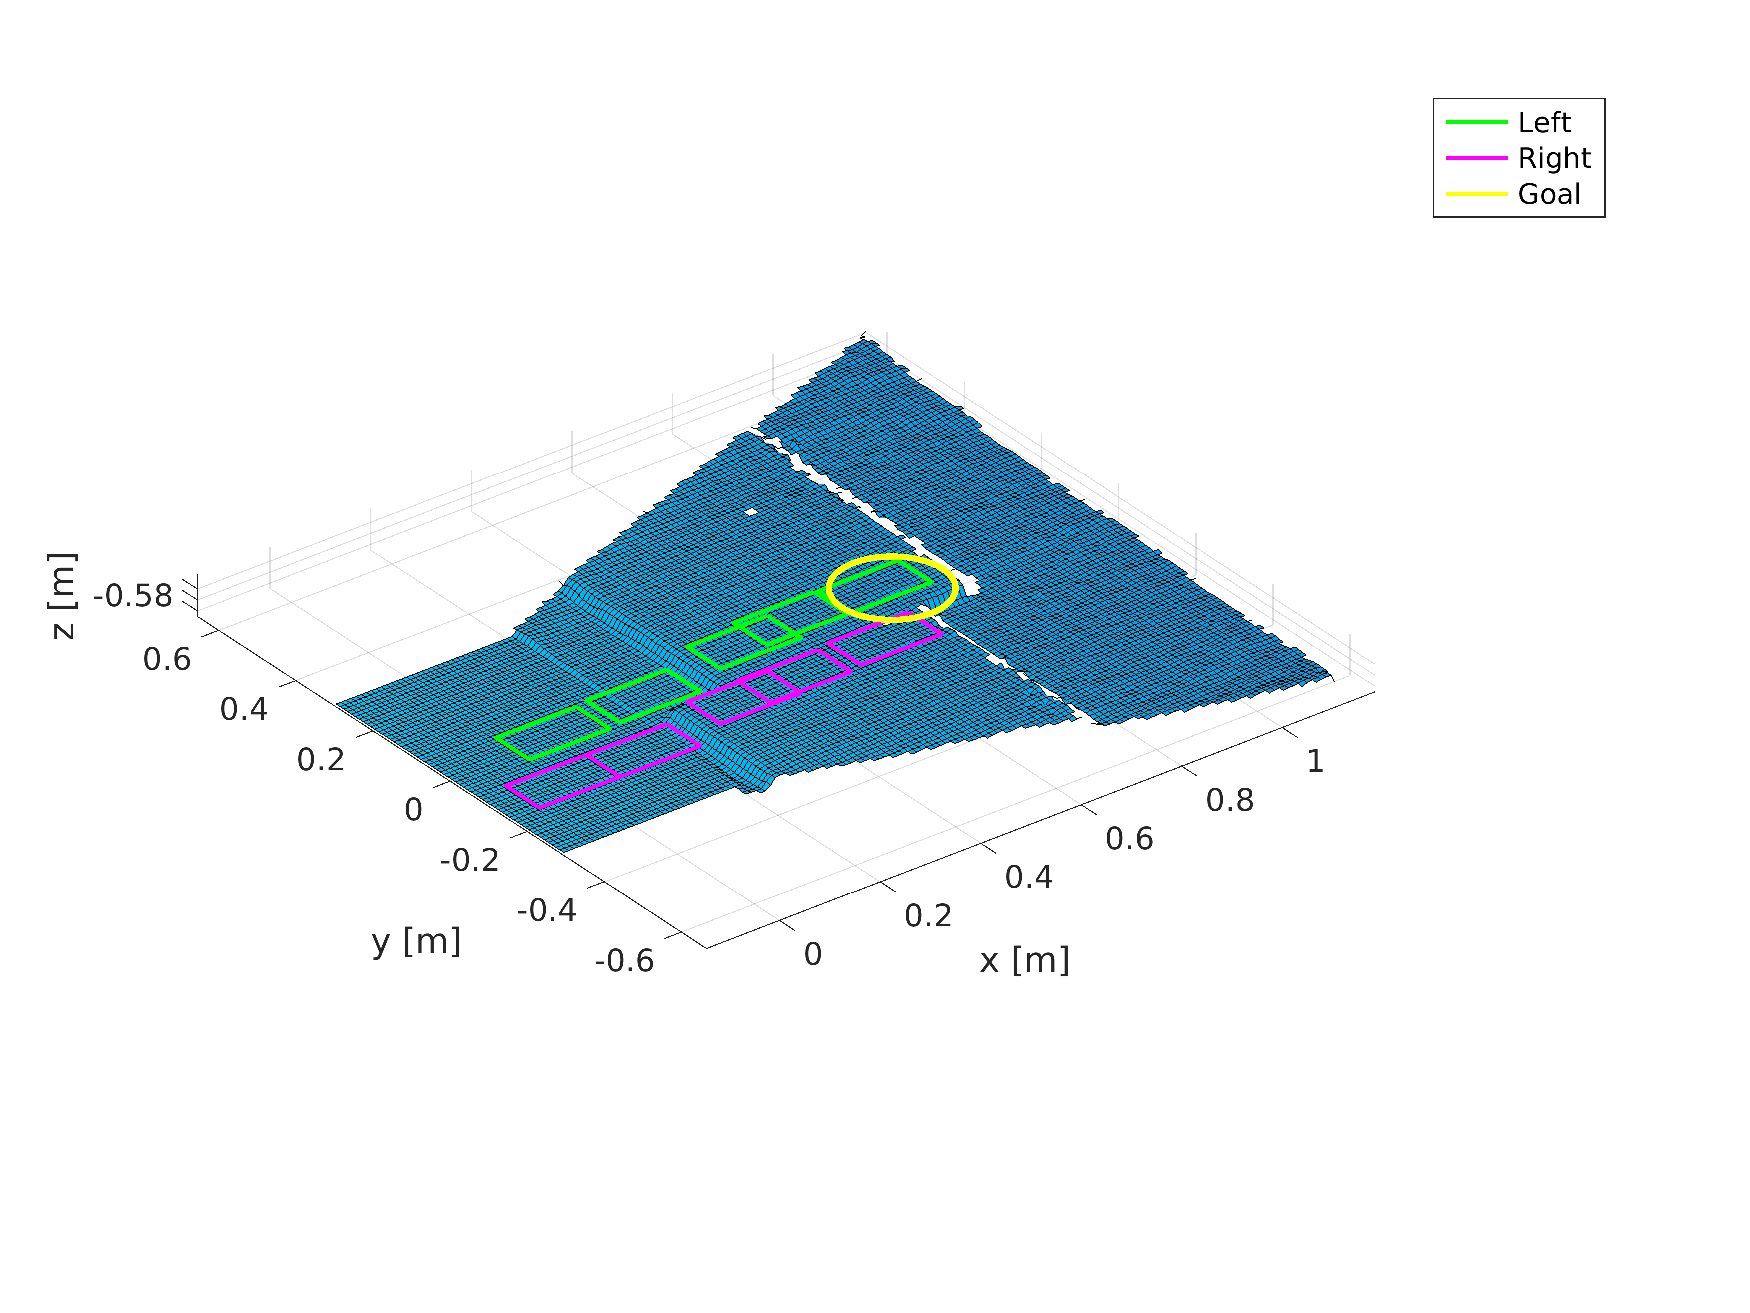
\includegraphics[width=0.95\textwidth]
        {figures/experiments/unknown-env/footstep-plan.pdf}
    \caption{Footstep plan generated for the scenario ``Stair Climbing in 
        Unknown Environments''.}
    \label{fig:experiments:unknown-env:footstep-plan}
\end{figure}
\begin{figure}
    \centering
    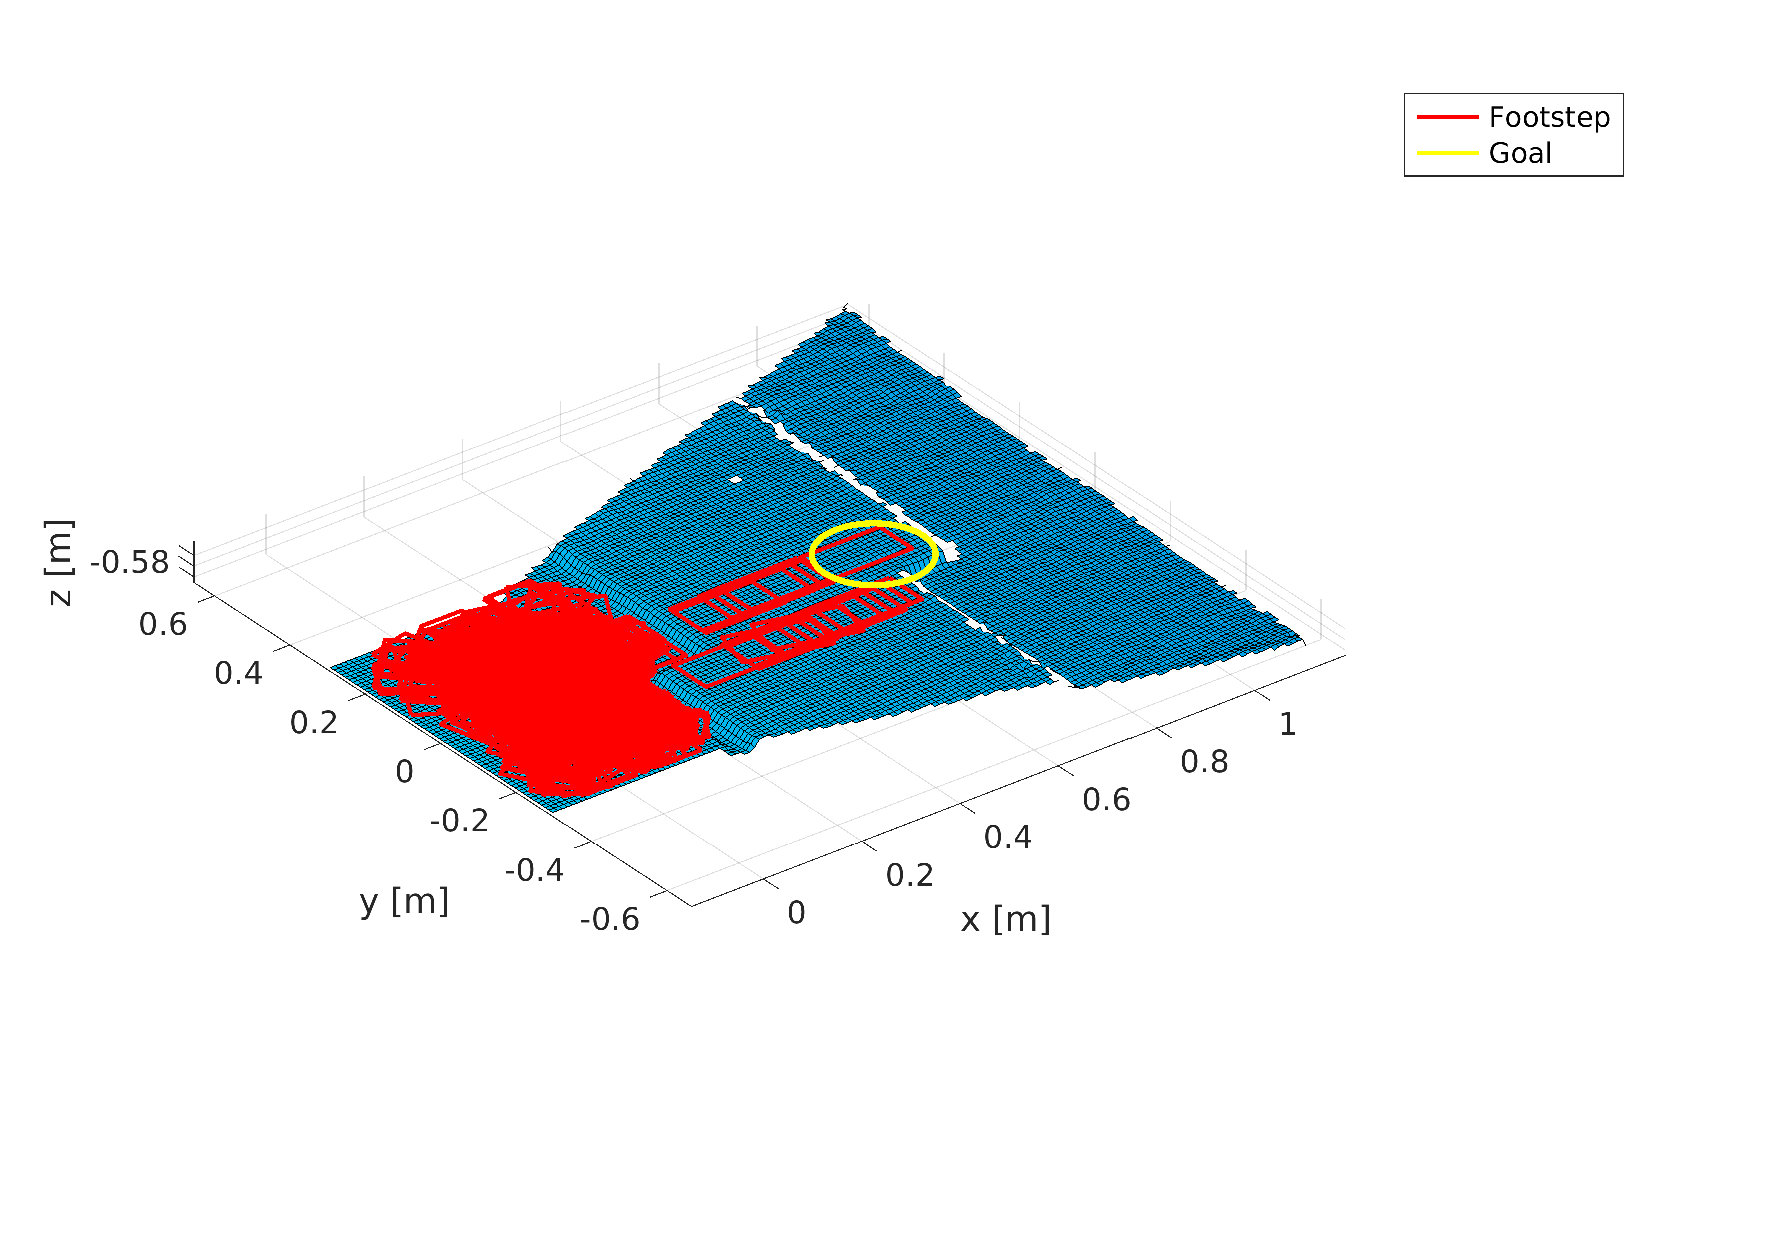
\includegraphics[width=0.95\textwidth]
        {figures/experiments/unknown-env/rrt-tree.pdf}
    \caption{Tree generated for the scenario ``Stair Climbing in 
        Unknown Environments''.}
    \label{fig:experiments:unknown-env:rrt-tree}
\end{figure}

